%\appendix
\chapter{Appendix}
\FloatBarrier
\section{Extended Result}
\FloatBarrier
\subsection{Set Estimation}\label{eresult:setest}
\FloatBarrier
Estimation using the techniques with different models are illustrated using data for one particular vehicle in the dataset in this chapter. Results show that the true state is always bounded by the set of estimation. For acceleration, there is no true measurement because the acceleration of the tracked vehicle is absent in the dataset.

\subsubsection{Segment Minimization using F-Radius}
\FloatBarrier
\begin{figure}[h]
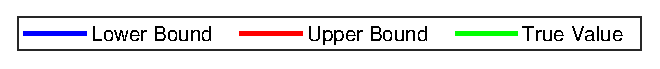
\includegraphics[scale=0.8]{figures/legend}\\\\
\begin{subfigure}{.5\linewidth}
\centering
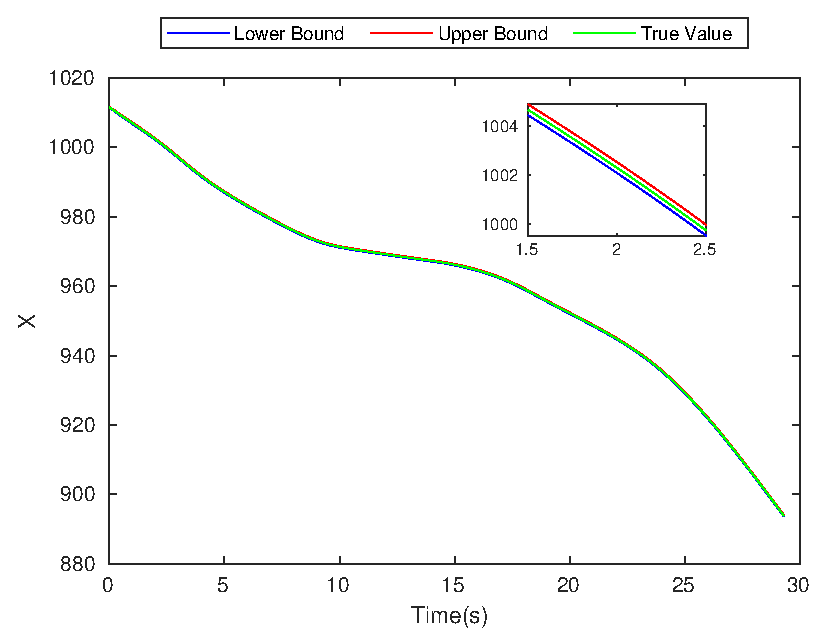
\includegraphics[width=\linewidth]{figures/Frad/s3cvSMX}
\end{subfigure}
\begin{subfigure}{.5\linewidth}
\centering
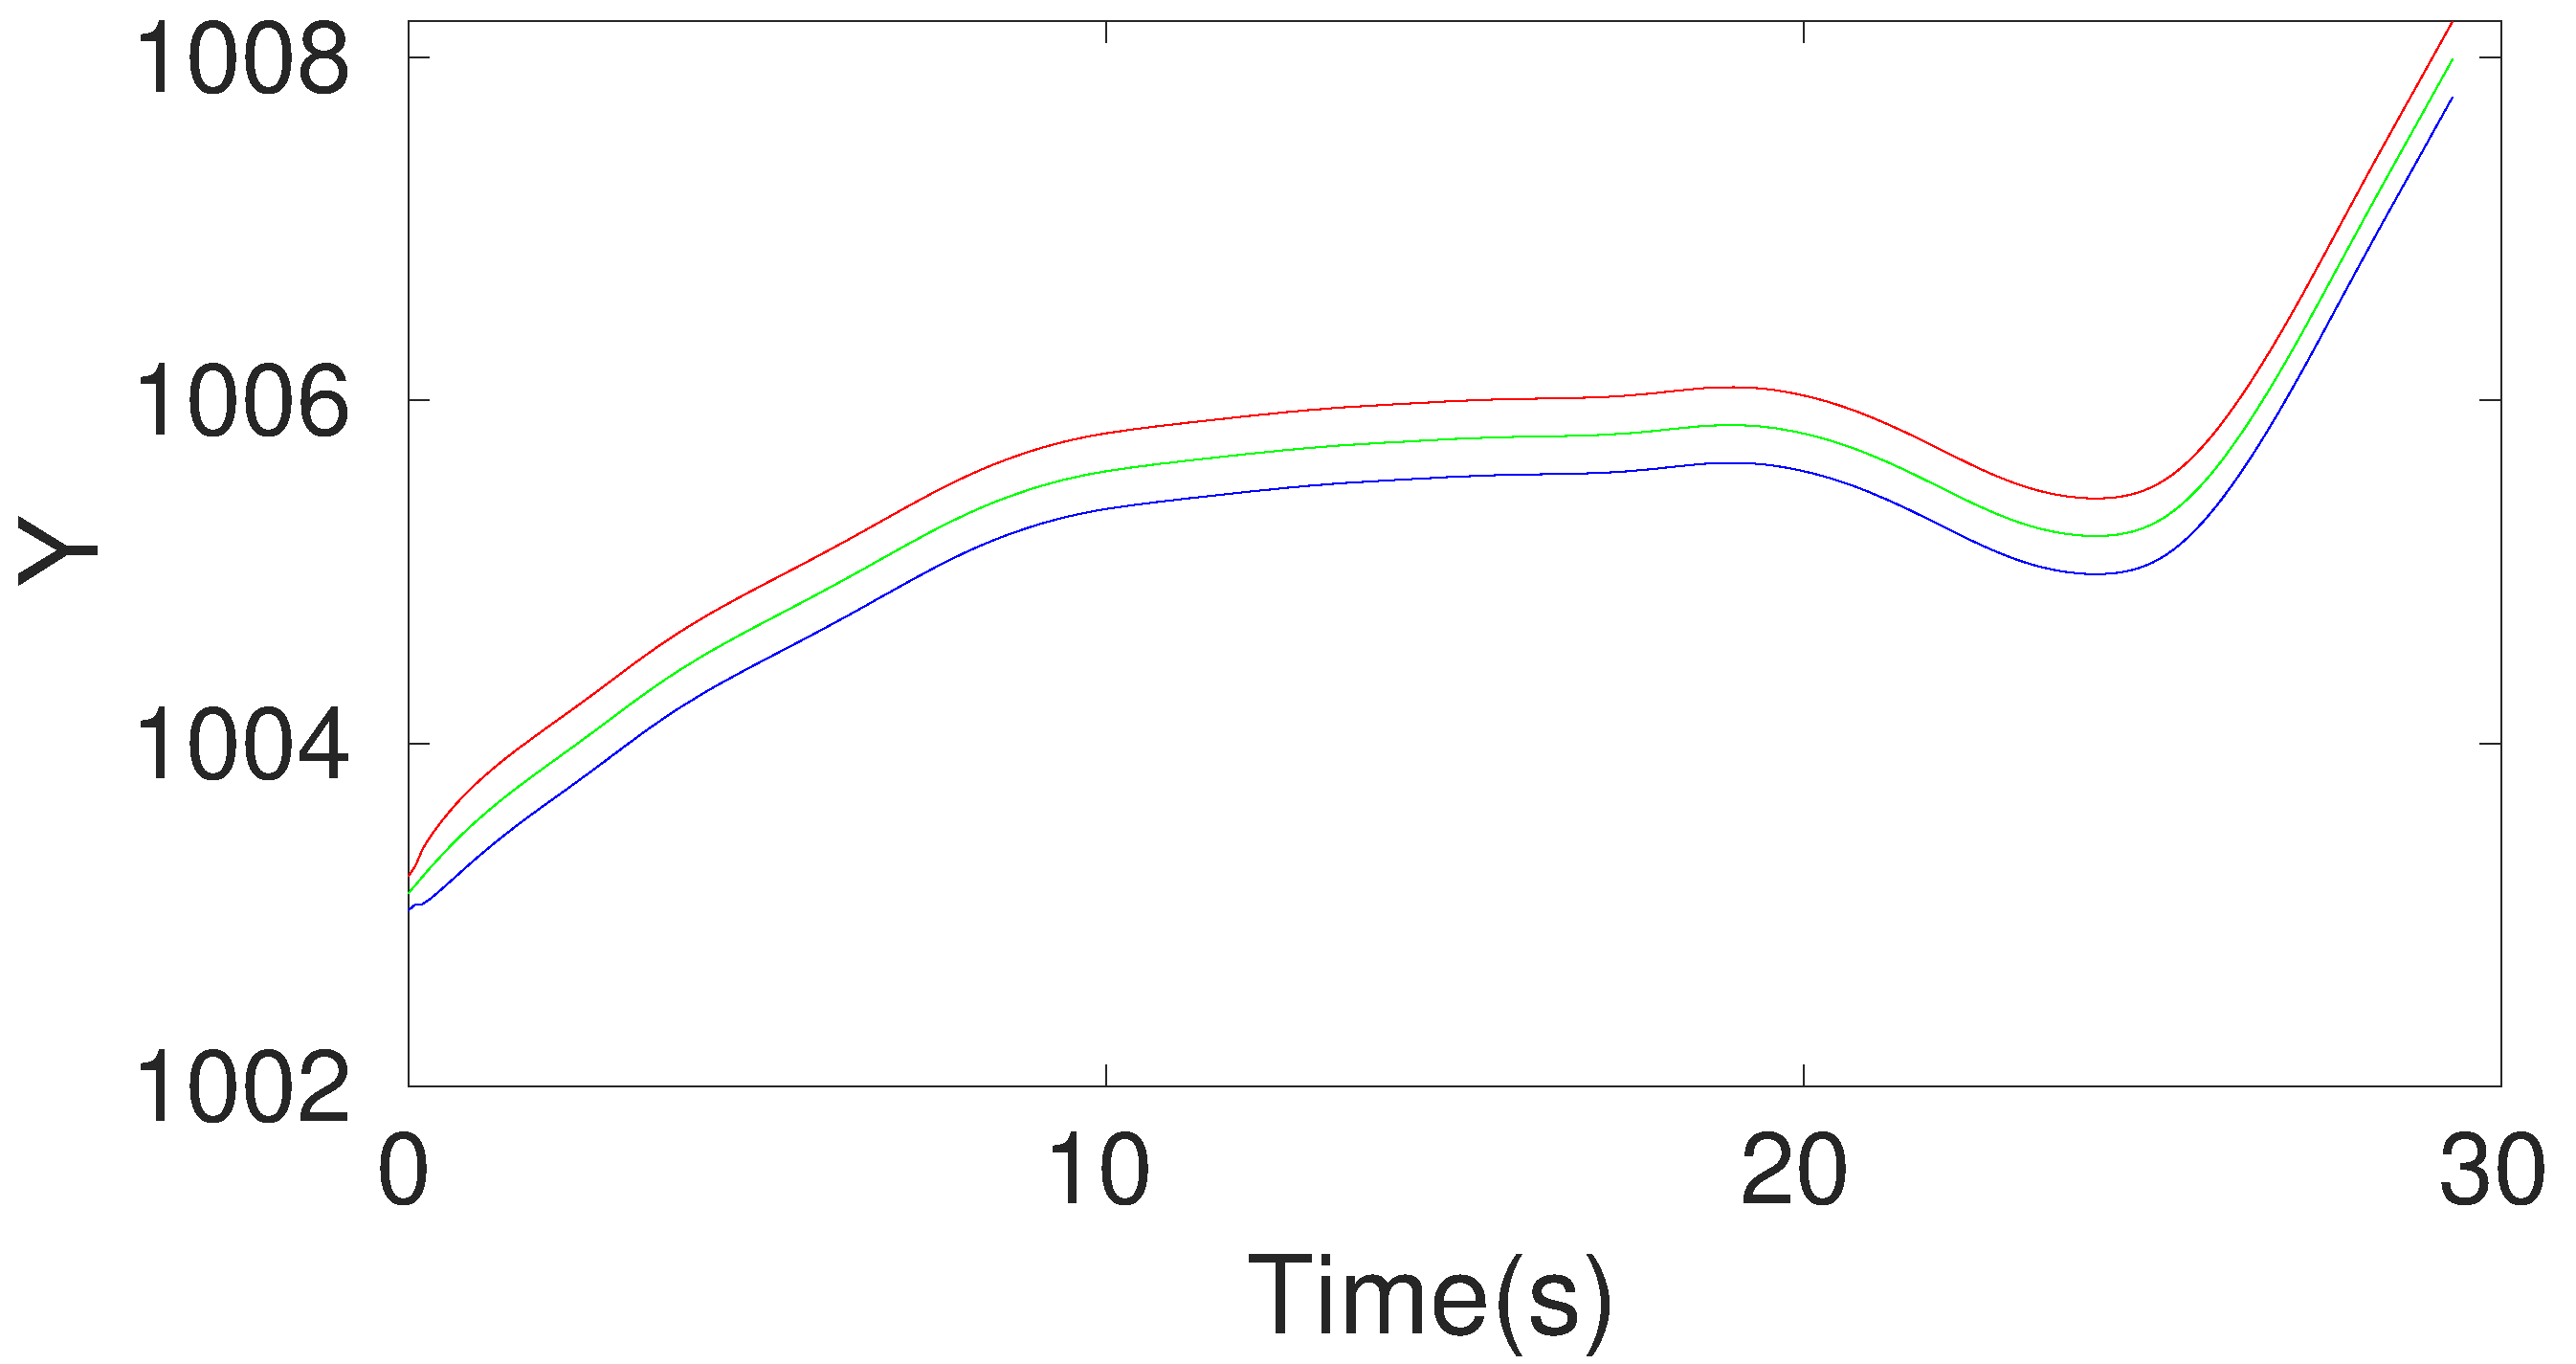
\includegraphics[width=\linewidth]{figures/Frad/s3cvSMY}
\end{subfigure}
\begin{subfigure}{.5\linewidth}
\centering
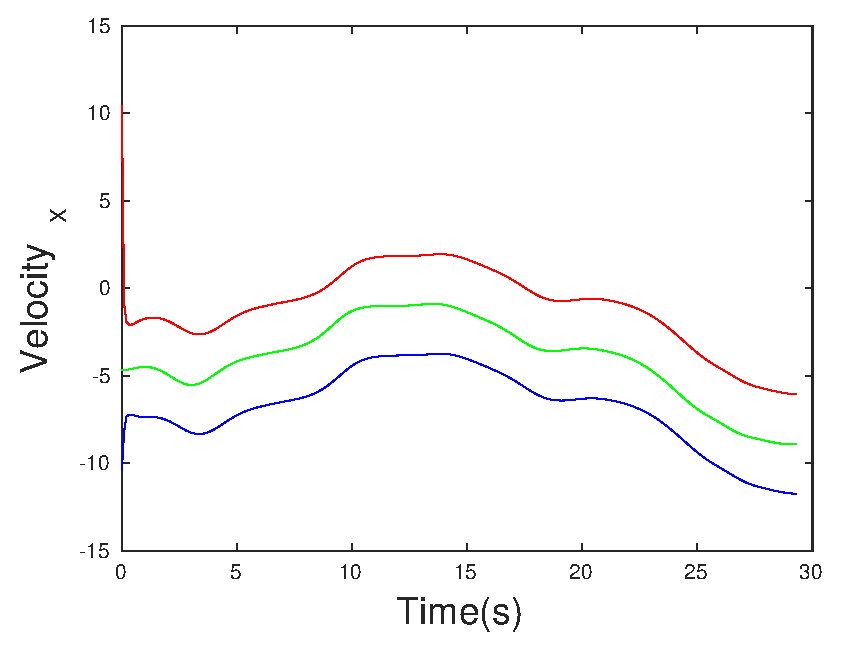
\includegraphics[width=\linewidth]{figures/Frad/s3cvSMVelocity_x}
\end{subfigure}
\begin{subfigure}{.5\linewidth}
\centering
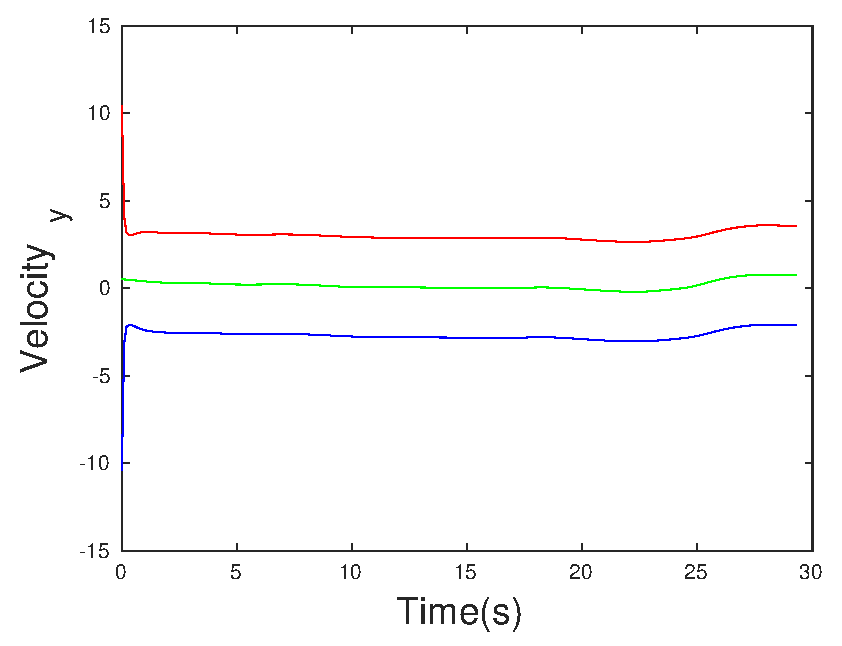
\includegraphics[width=\linewidth]{figures/Frad/s3cvSMVelocity_y}
\end{subfigure}
\caption{Estimation using Constant Velocity}
\end{figure}

\begin{figure}[h]
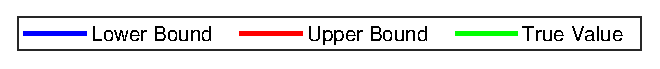
\includegraphics[scale=0.8]{figures/legend}\\\\
\begin{subfigure}{.5\linewidth}
\centering
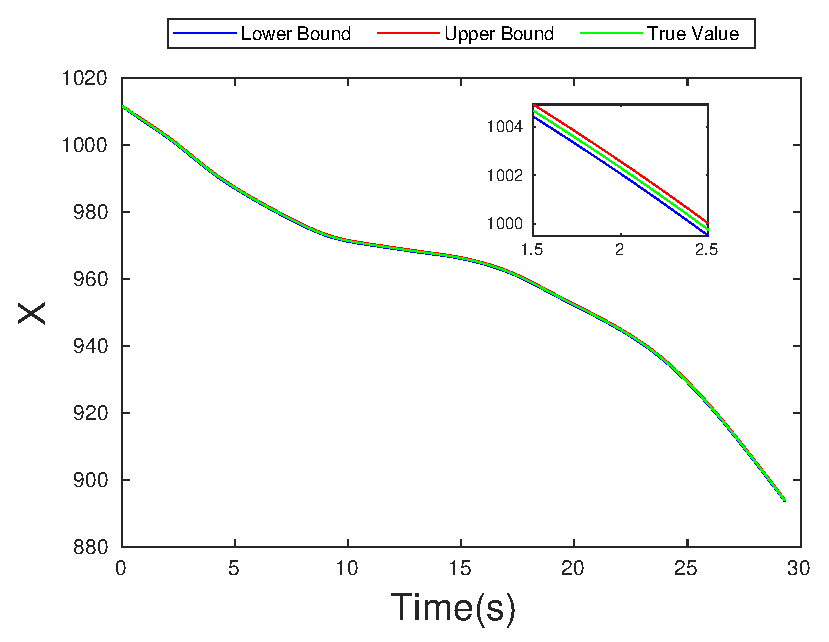
\includegraphics[width=\linewidth]{figures/Frad/s3caSMX}
\end{subfigure}
\begin{subfigure}{.5\linewidth}
\centering
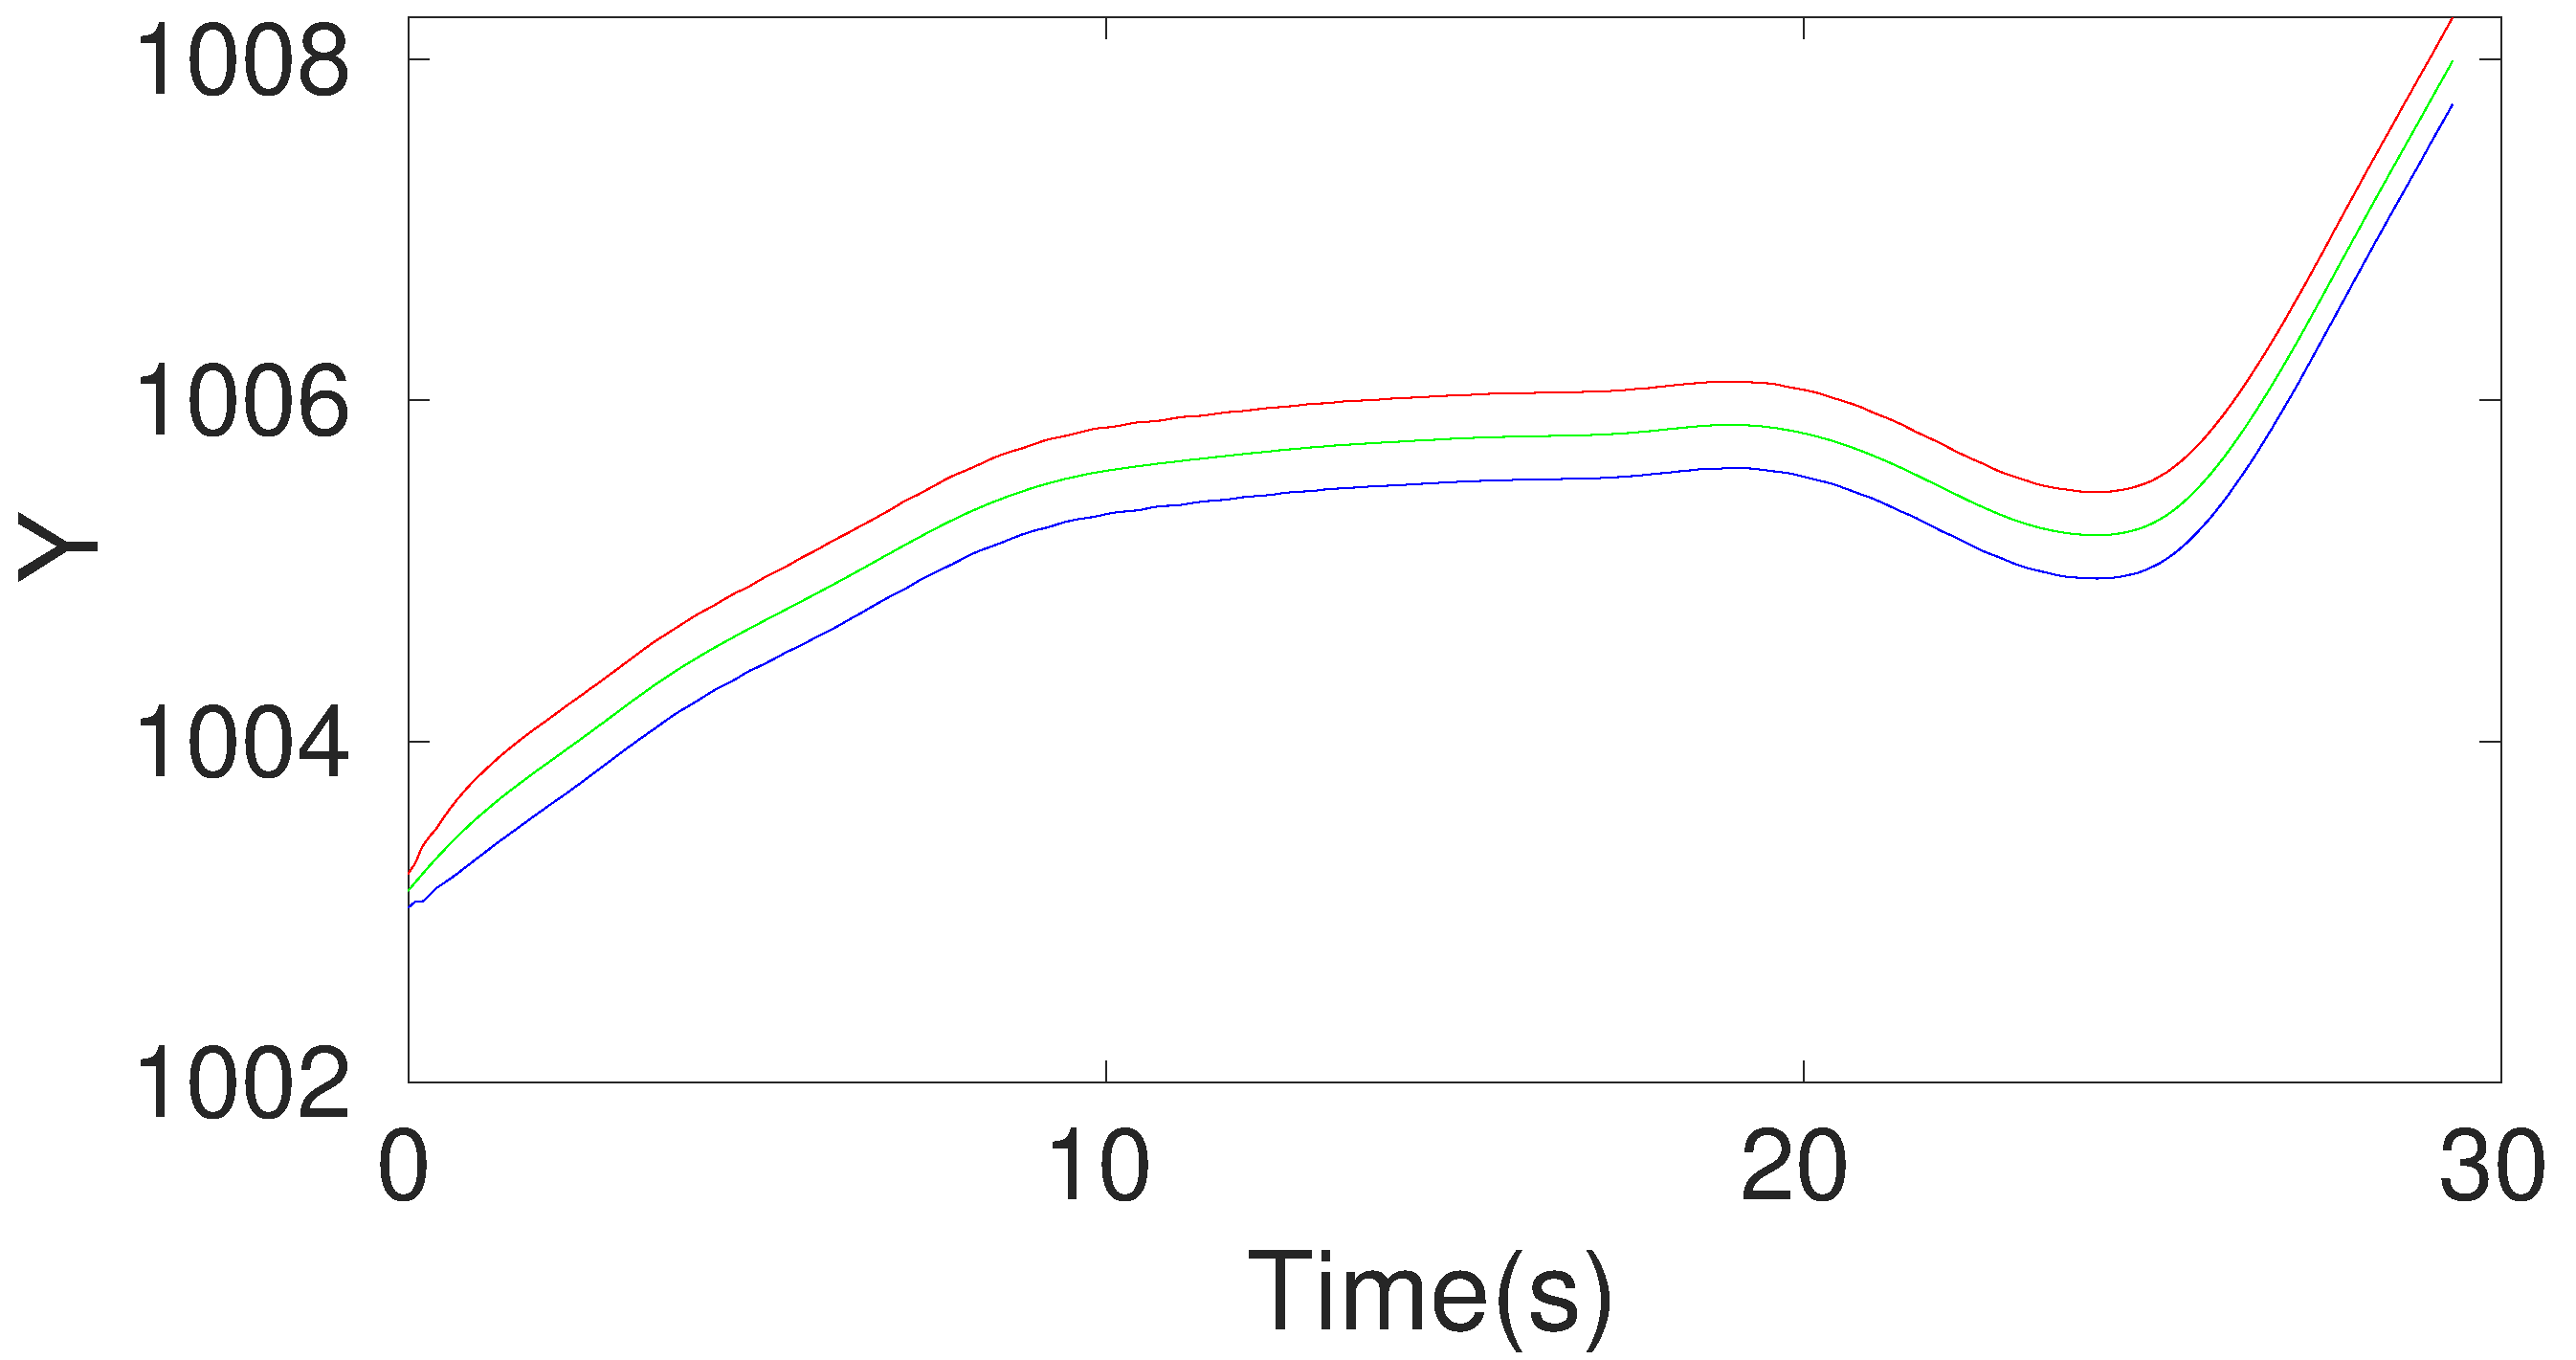
\includegraphics[width=\linewidth]{figures/Frad/s3caSMY}
\end{subfigure}
\begin{subfigure}{.5\linewidth}
\centering
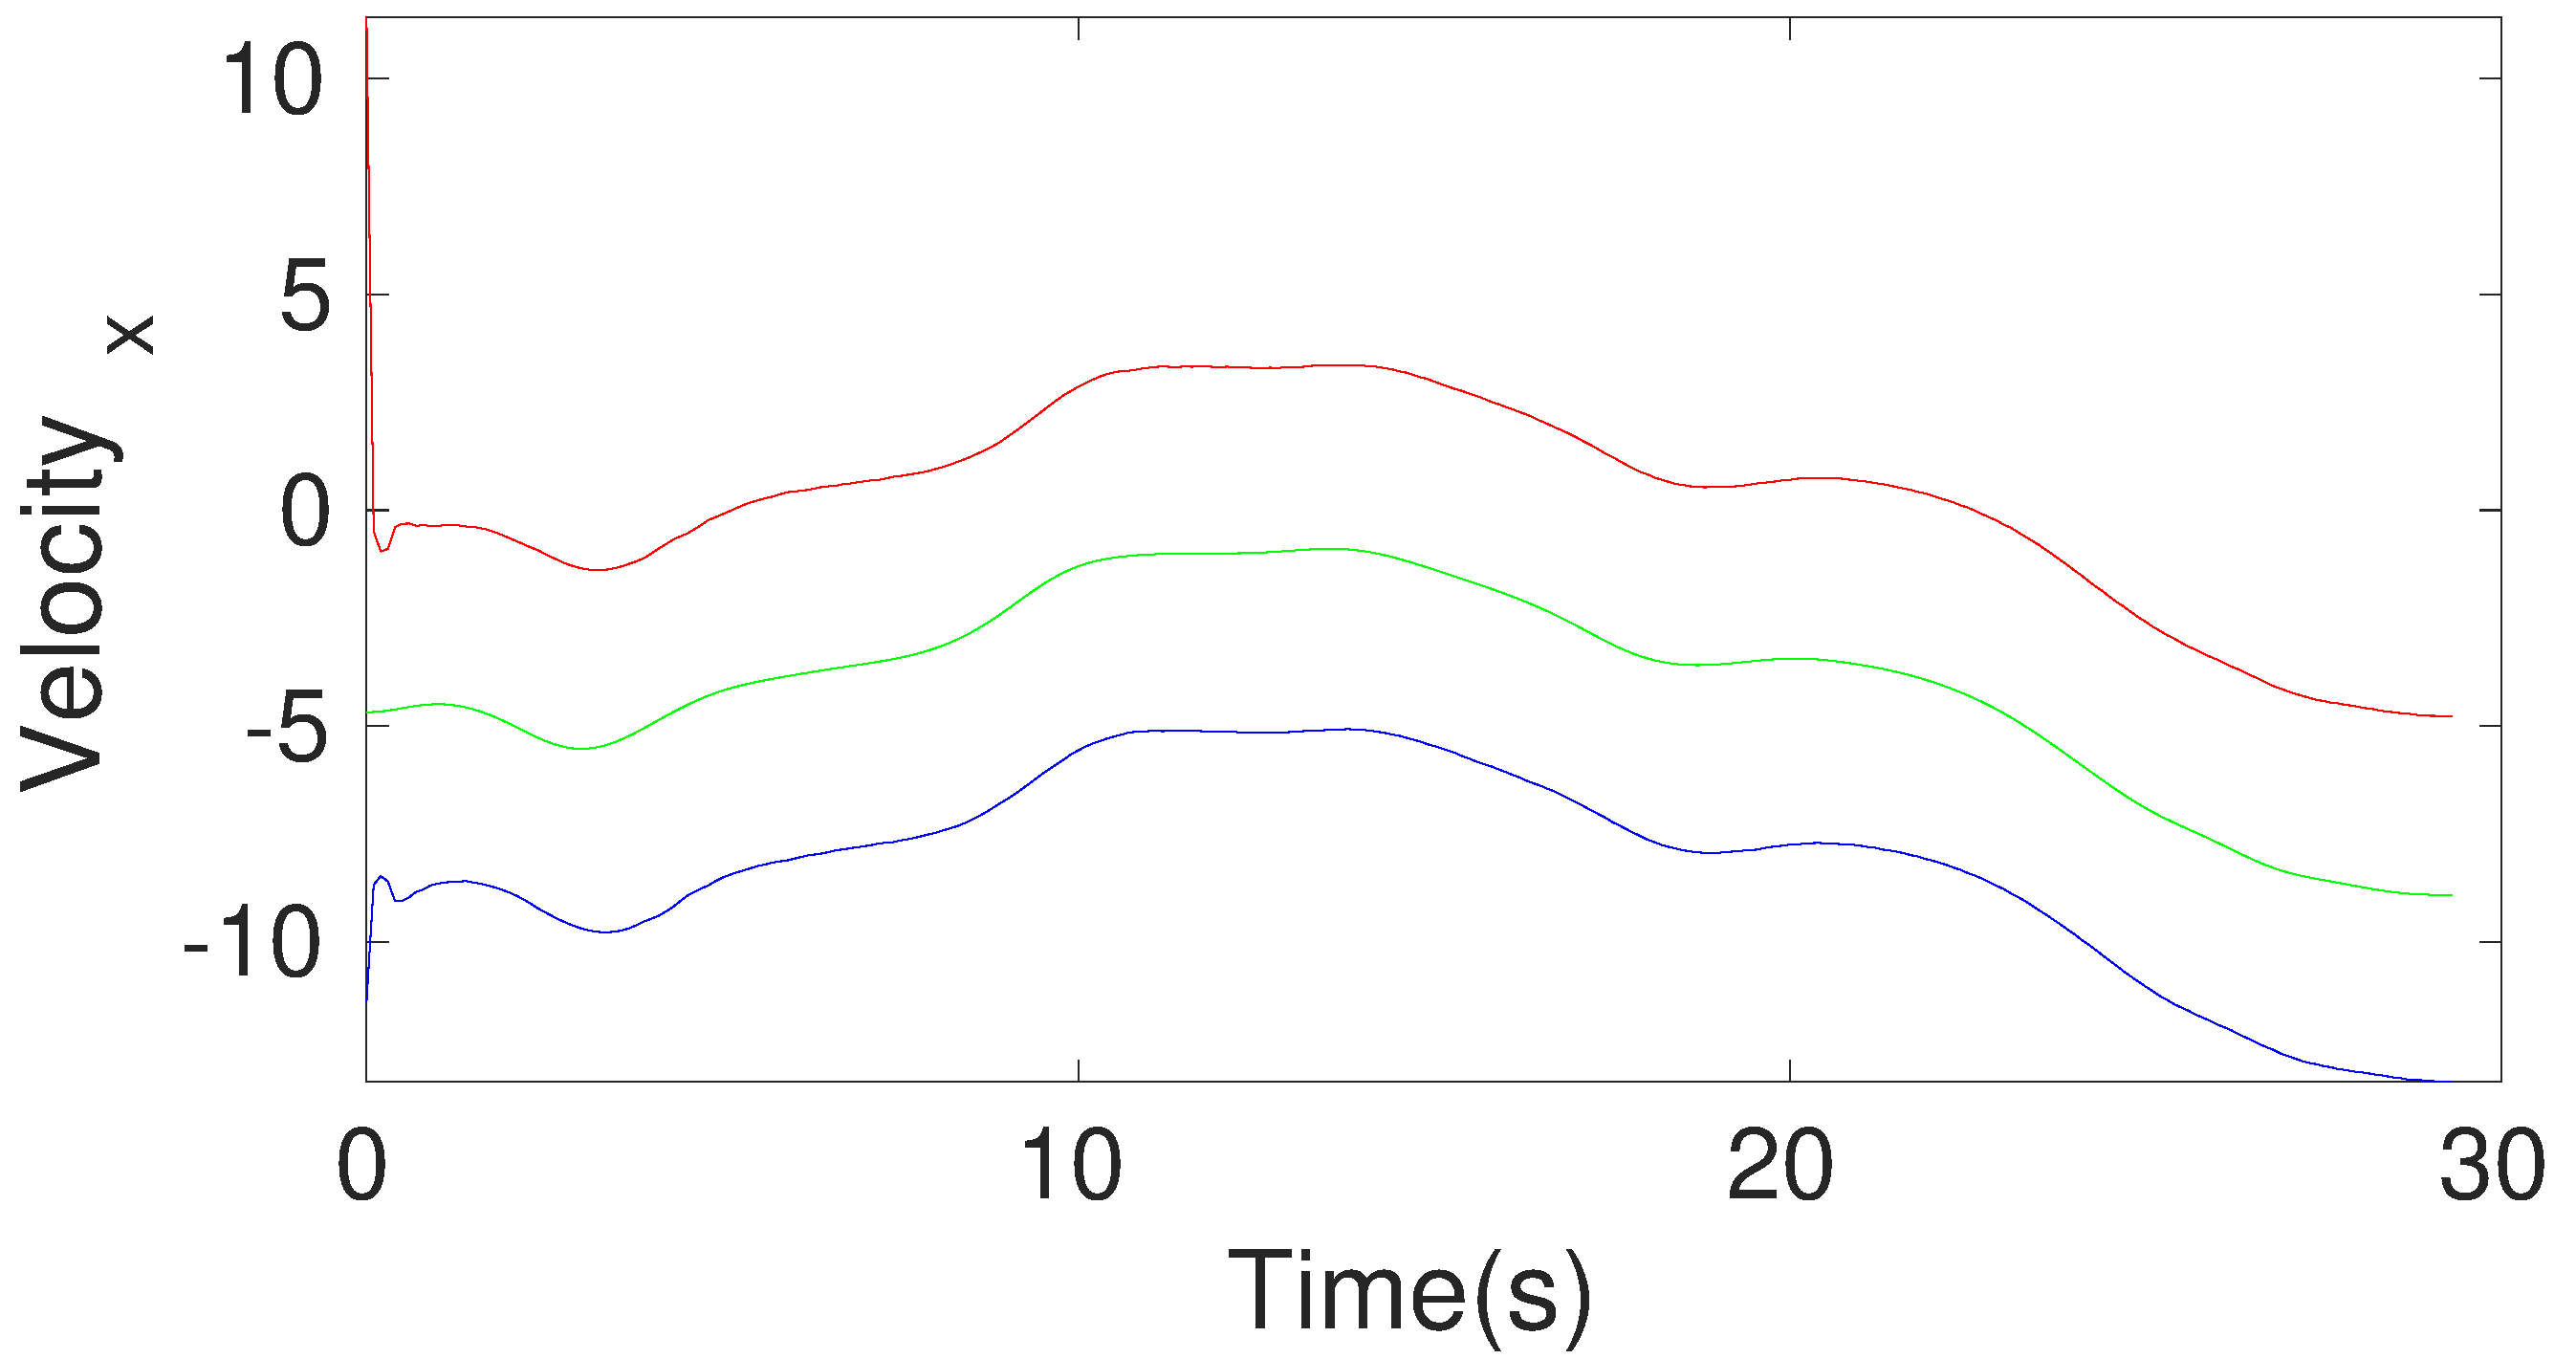
\includegraphics[width=\linewidth]{figures/Frad/s3caSMVelocity_x}
\end{subfigure}
\begin{subfigure}{.5\linewidth}
\centering
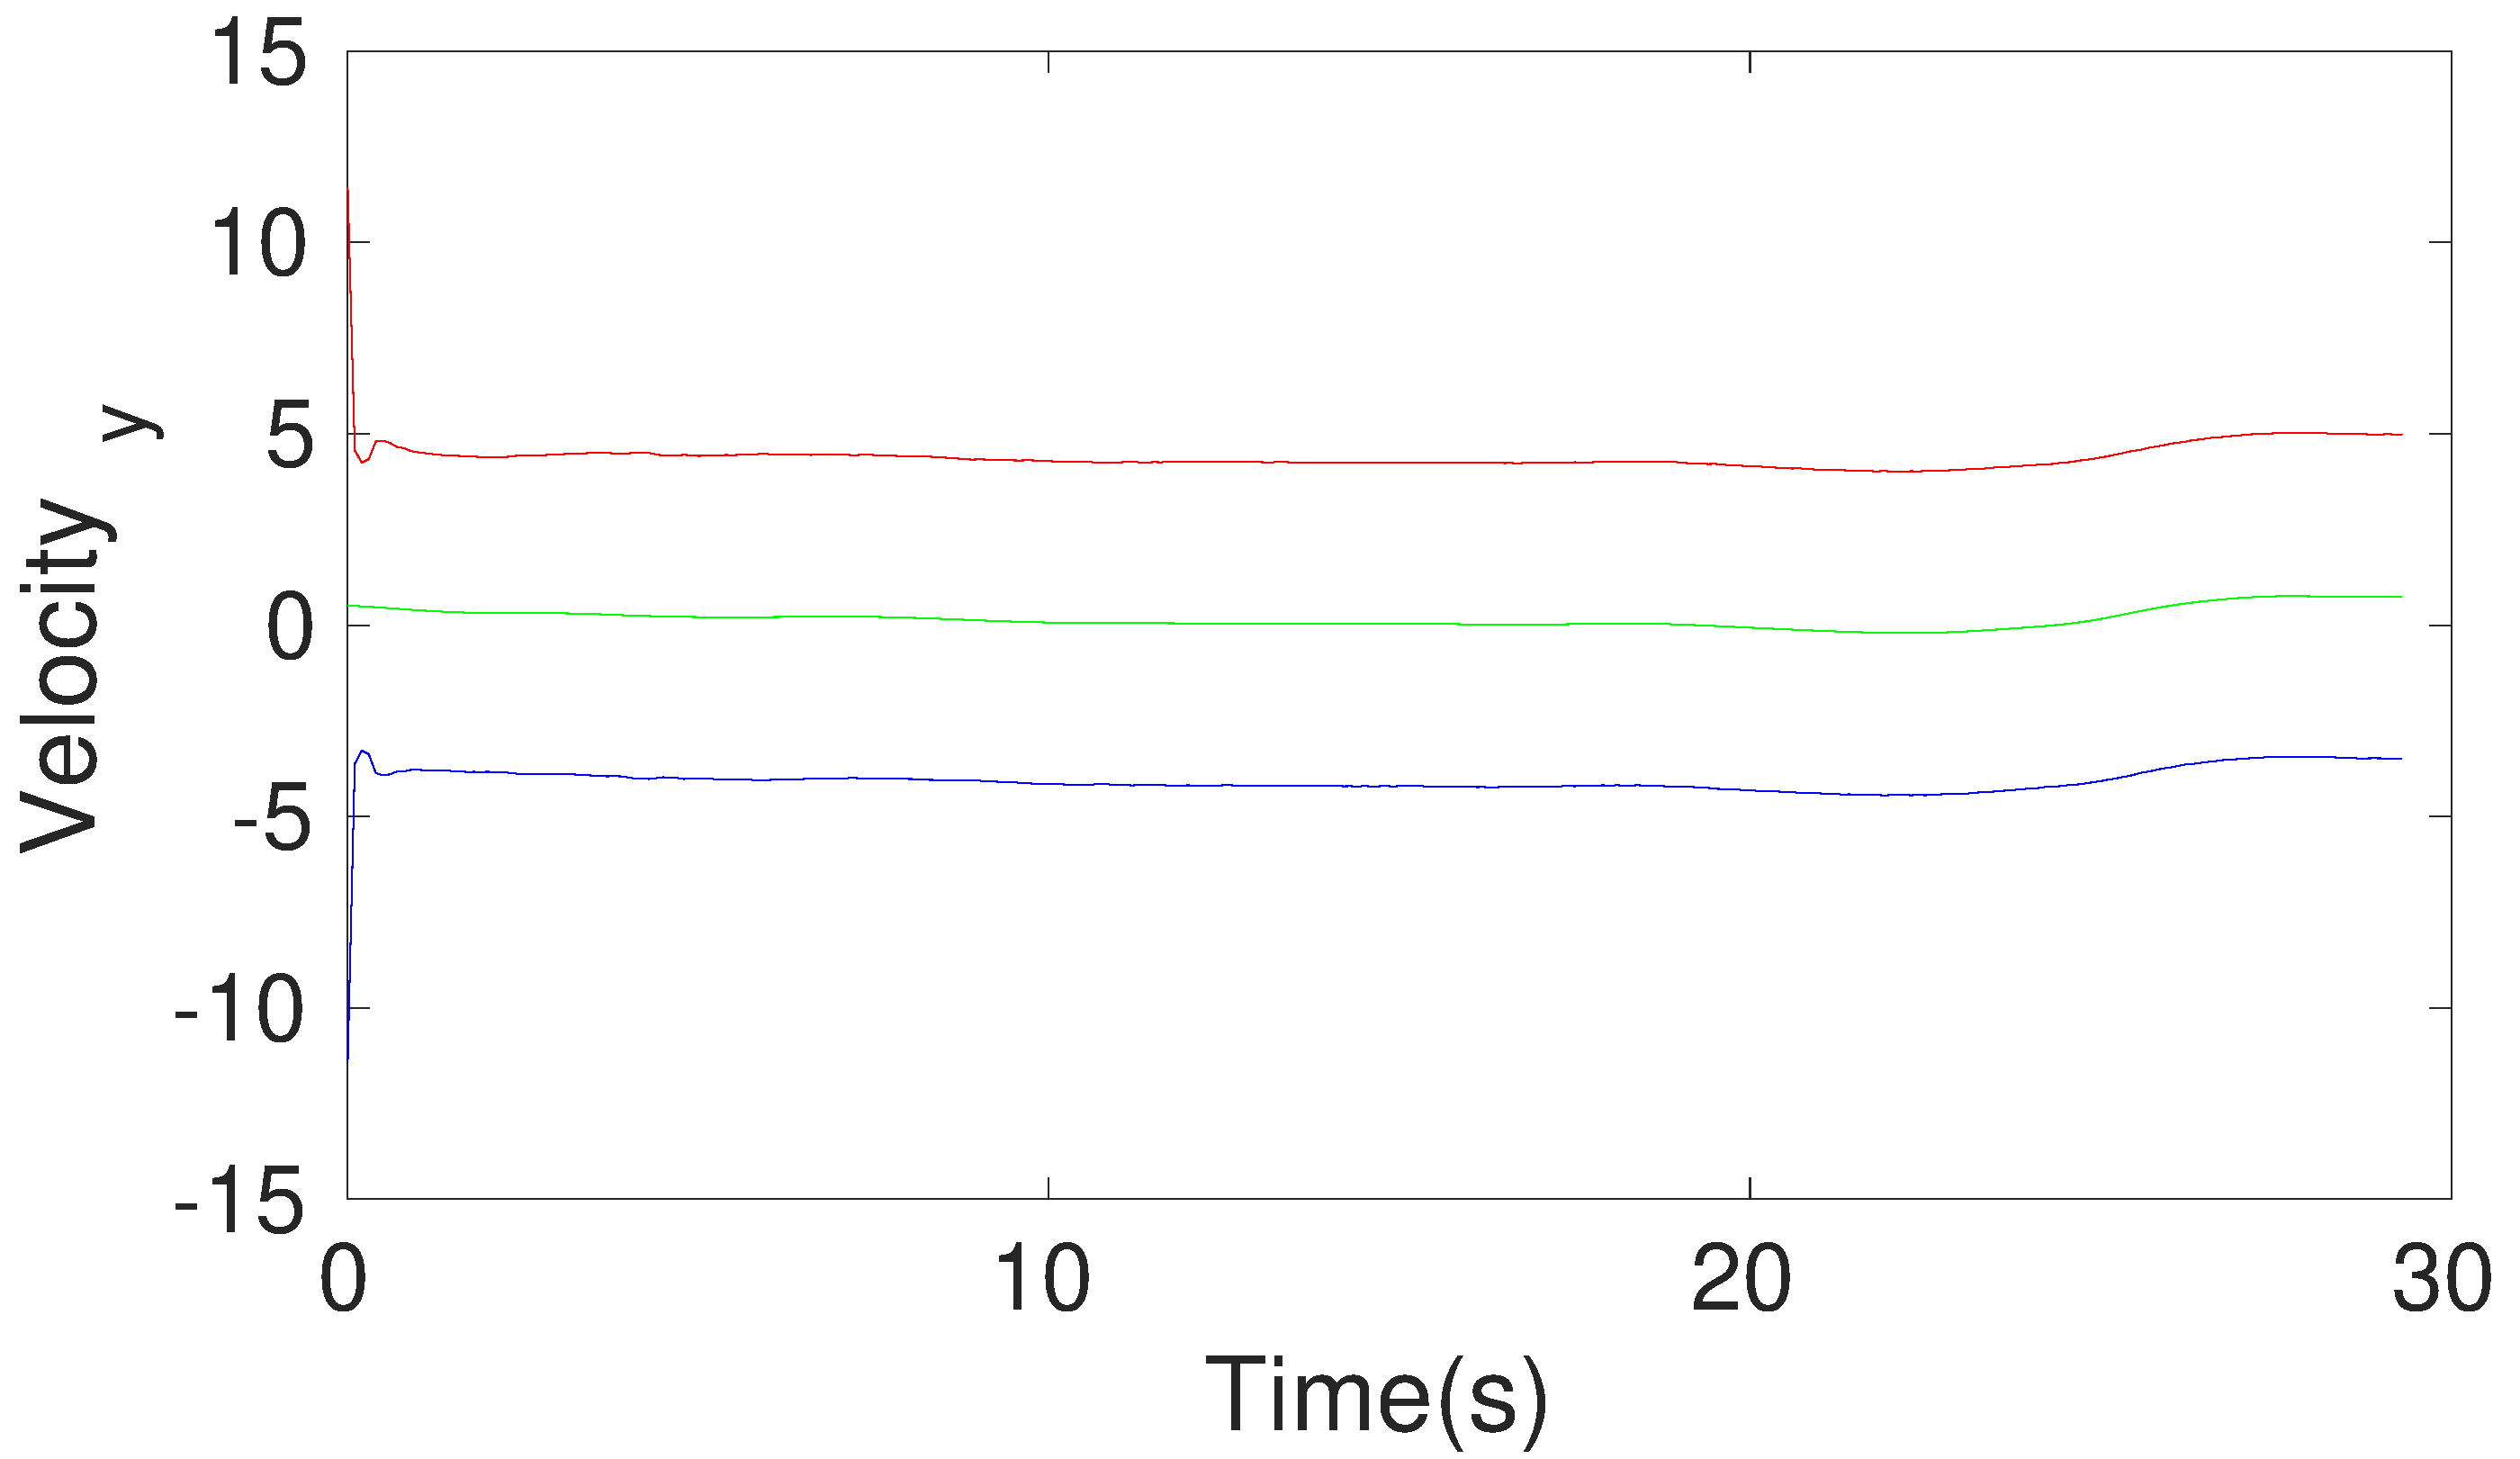
\includegraphics[width=\linewidth]{figures/Frad/s3caSMVelocity_y}
\end{subfigure}
\begin{subfigure}{.5\linewidth}
\centering
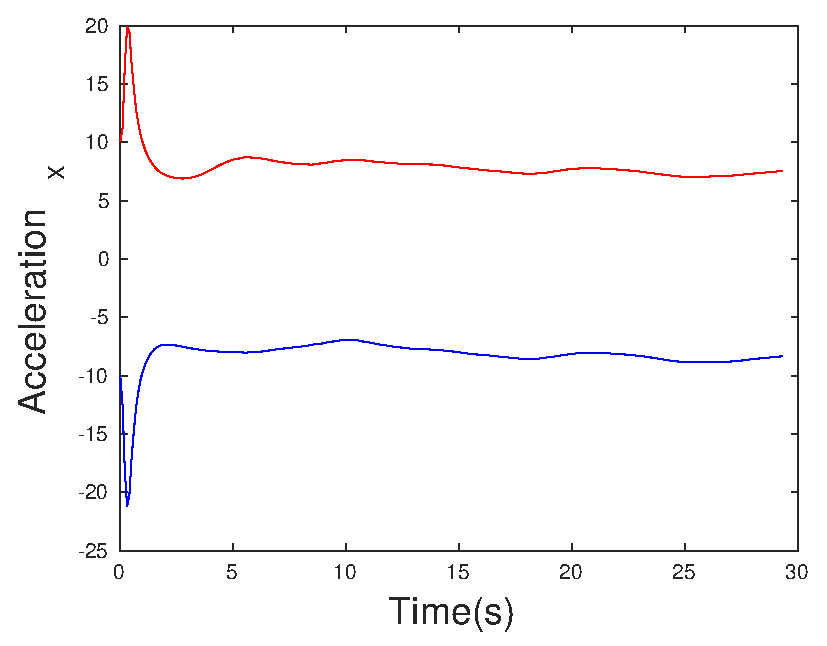
\includegraphics[width=\linewidth]{figures/Frad/s3caSMAcceleration_x}
\end{subfigure}
\begin{subfigure}{.5\linewidth}
\centering
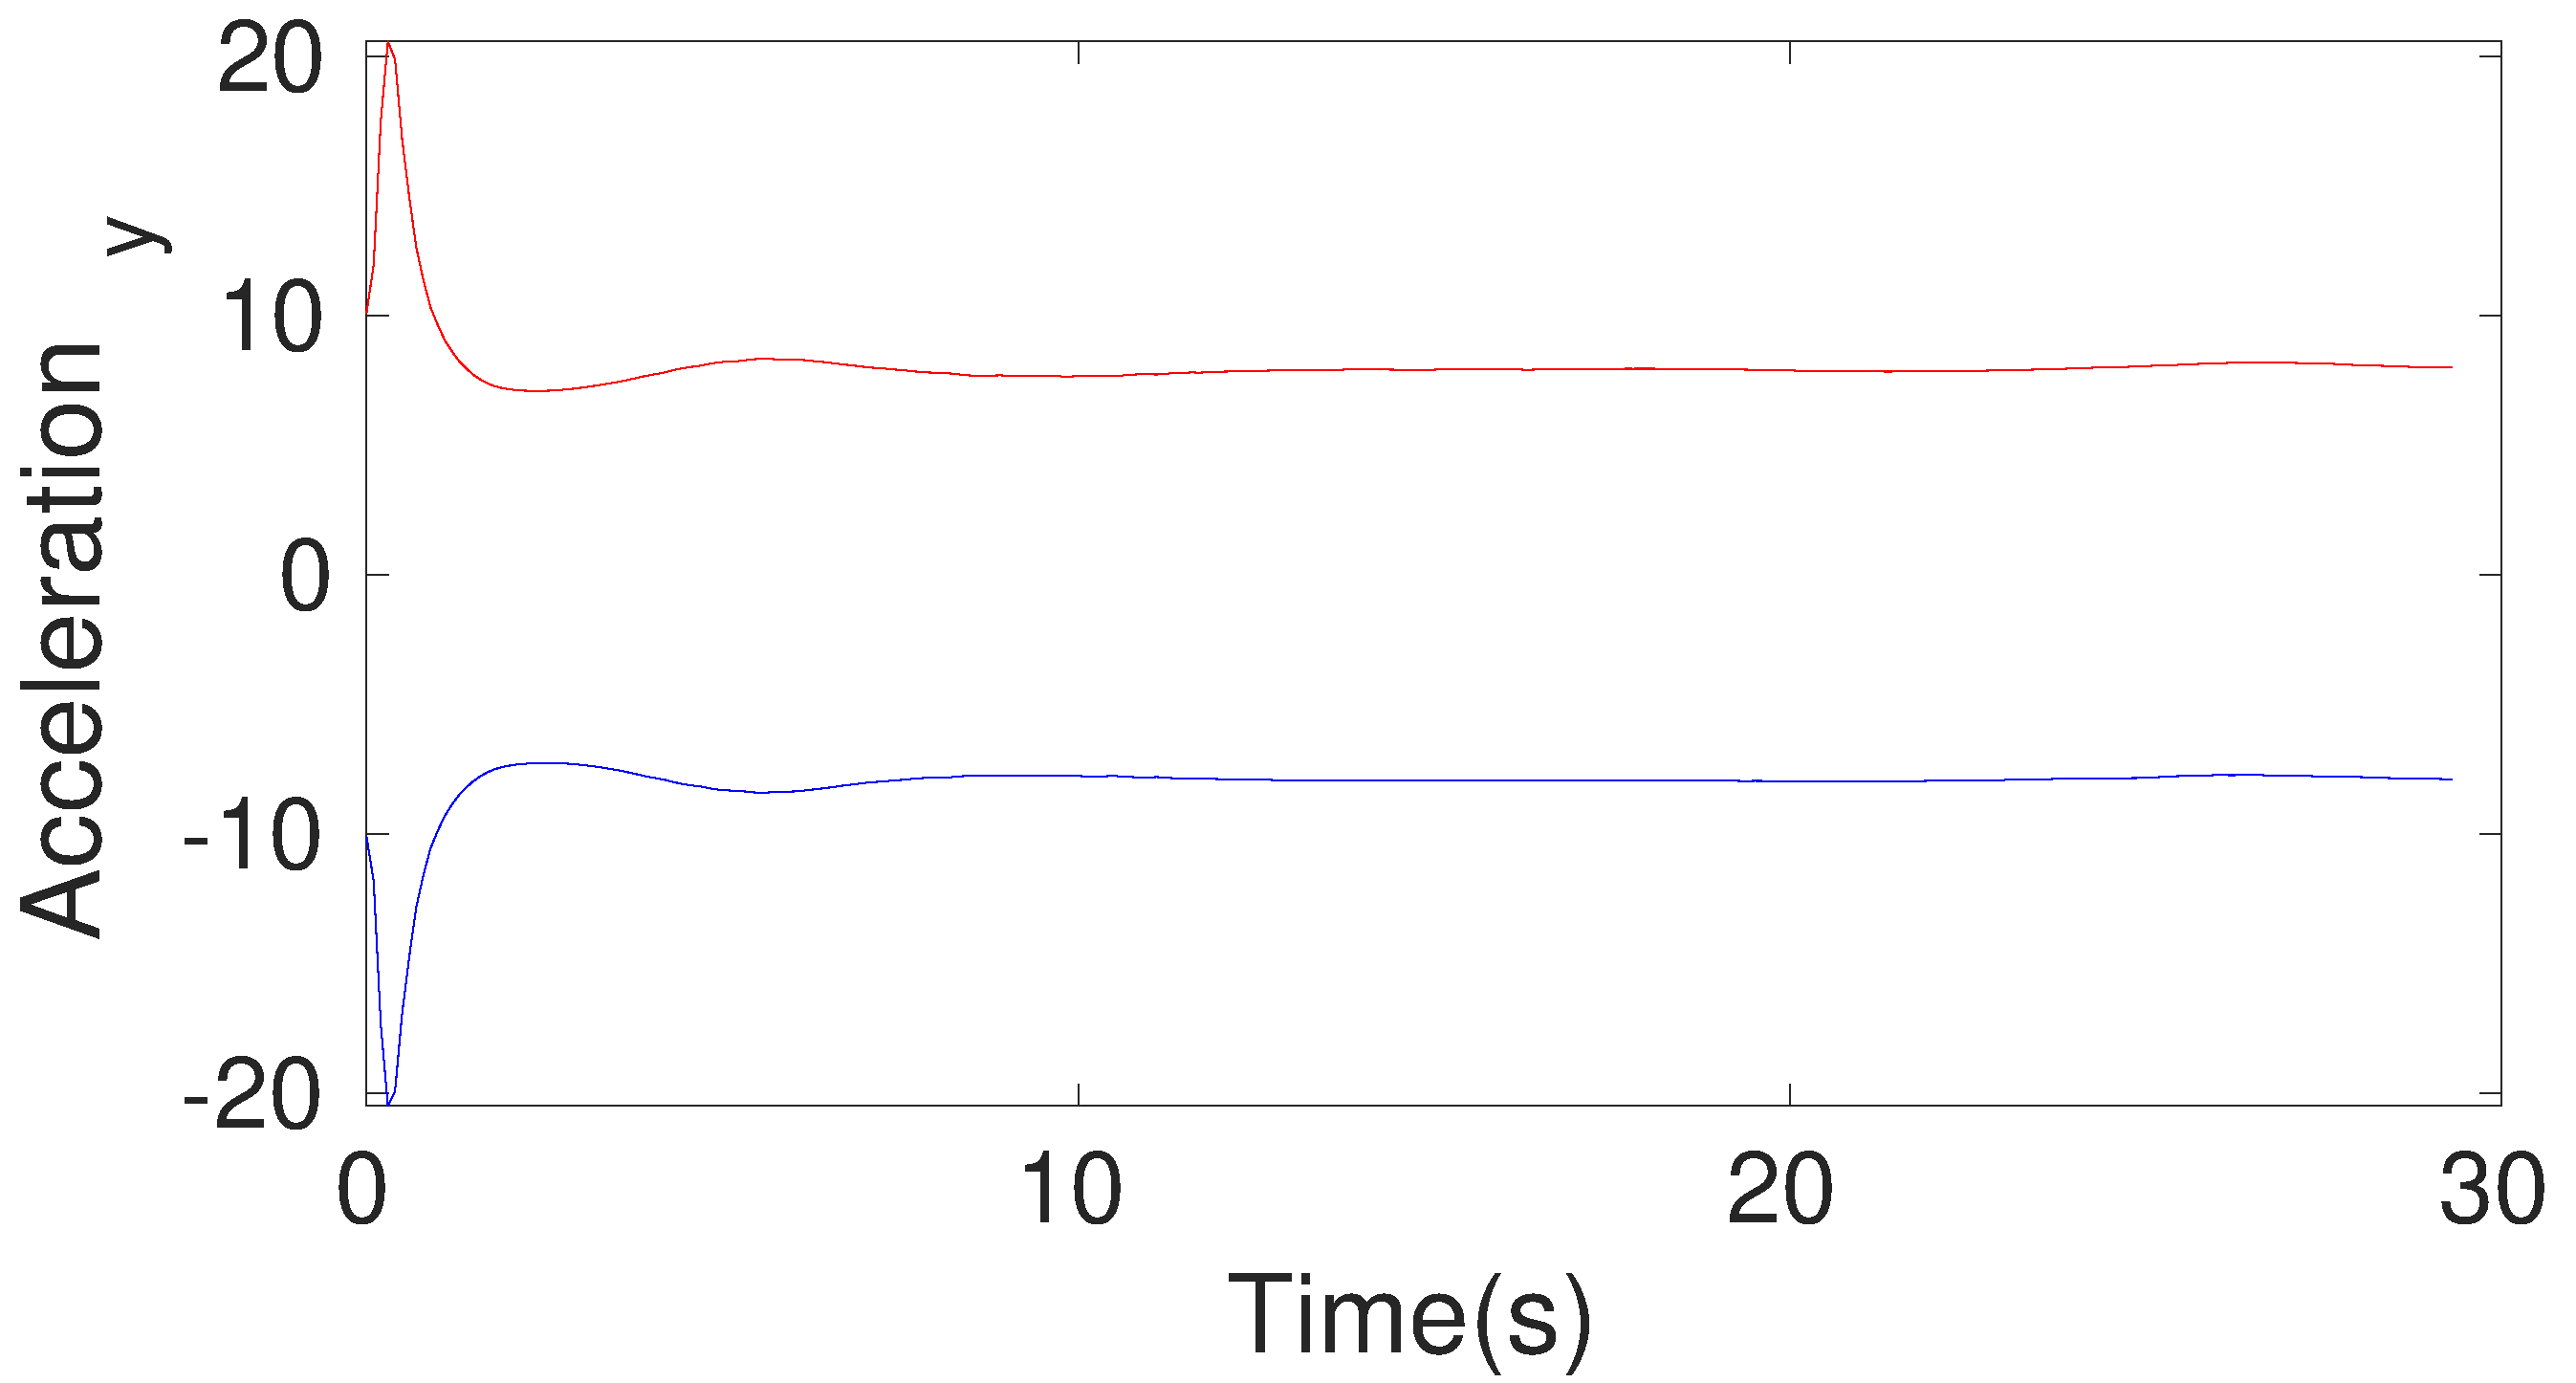
\includegraphics[width=\linewidth]{figures/Frad/s3caSMAcceleration_y}
\end{subfigure}
\caption{Estimation using Constant Acceleration}
\end{figure}

\begin{figure}[h]
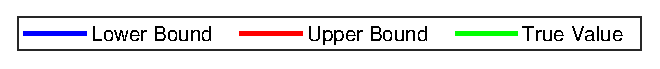
\includegraphics[scale=0.8]{figures/legend}\\\\
\begin{subfigure}{.5\linewidth}
\centering
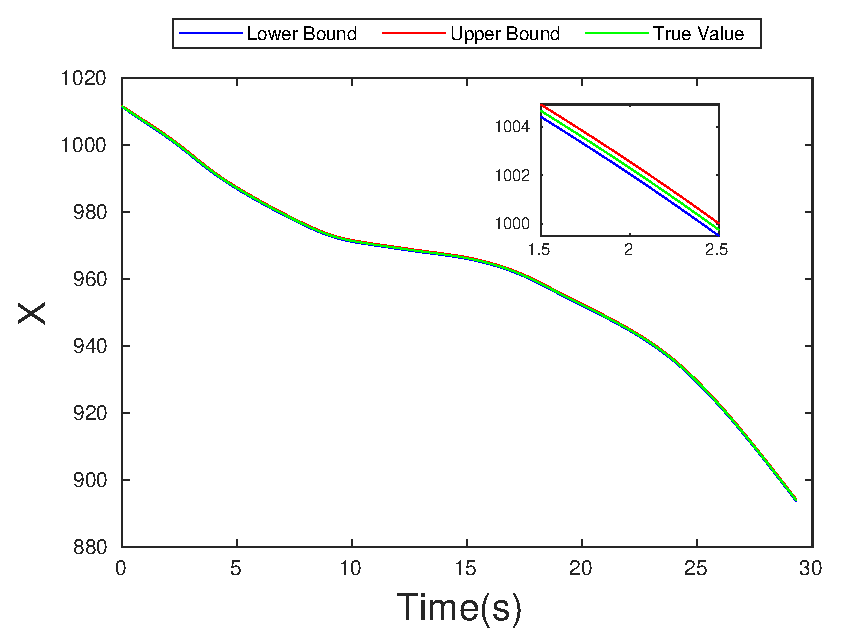
\includegraphics[width=\linewidth]{figures/Frad/s3pmSMX}
\end{subfigure}
\begin{subfigure}{.5\linewidth}
\centering
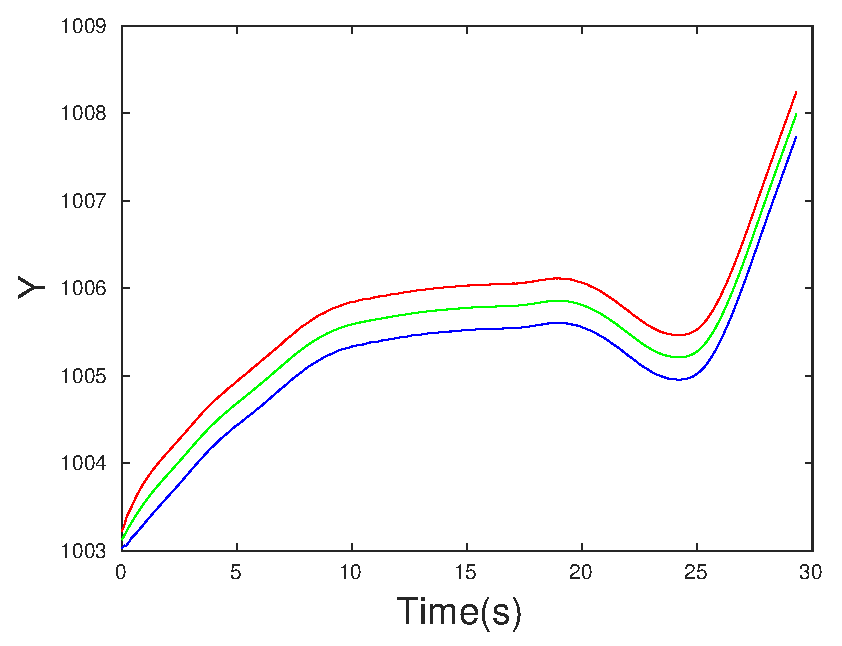
\includegraphics[width=\linewidth]{figures/Frad/s3pmSMY}
\end{subfigure}
\begin{subfigure}{.5\linewidth}
\centering
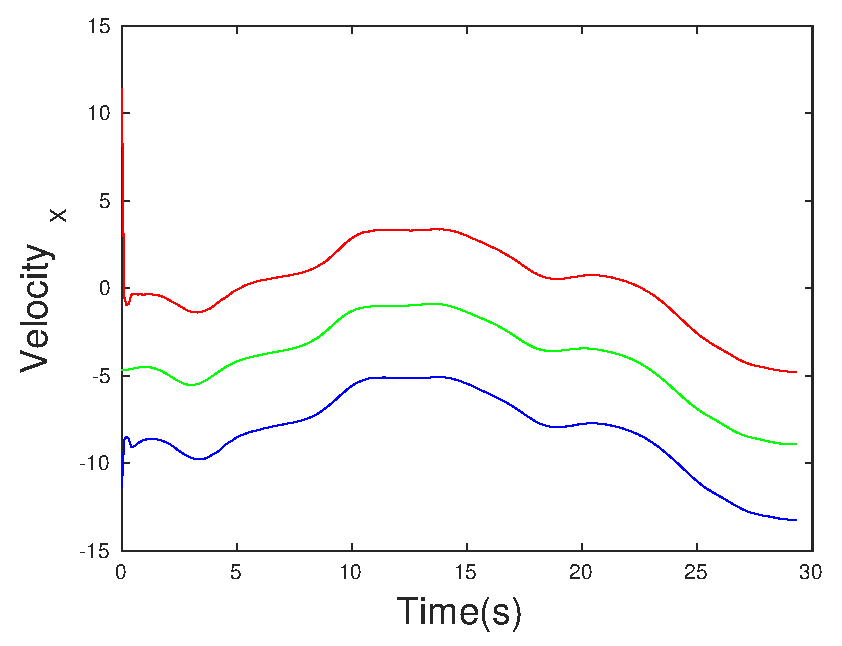
\includegraphics[width=\linewidth]{figures/Frad/s3pmSMVelocity_x}
\end{subfigure}
\begin{subfigure}{.5\linewidth}
\centering
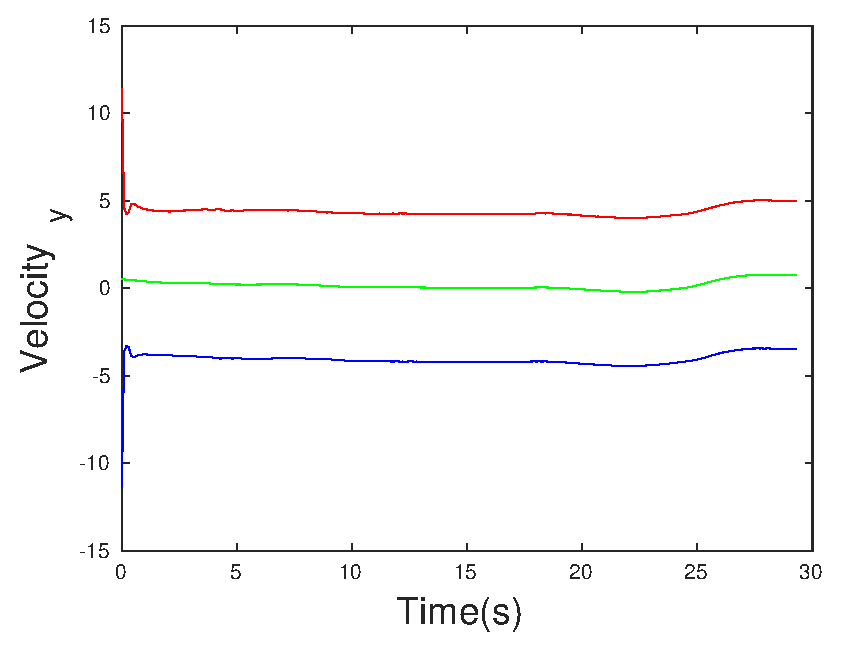
\includegraphics[width=\linewidth]{figures/Frad/s3pmSMVelocity_y}
\end{subfigure}
\begin{subfigure}{.5\linewidth}
\centering
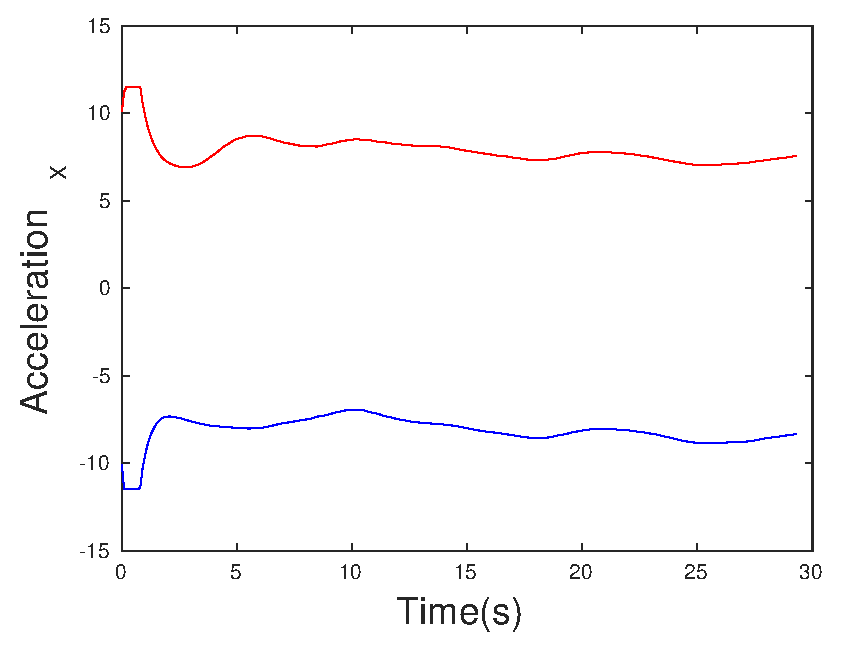
\includegraphics[width=\linewidth]{figures/Frad/s3pmSMAcceleration_x}
\end{subfigure}
\begin{subfigure}{.5\linewidth}
\centering
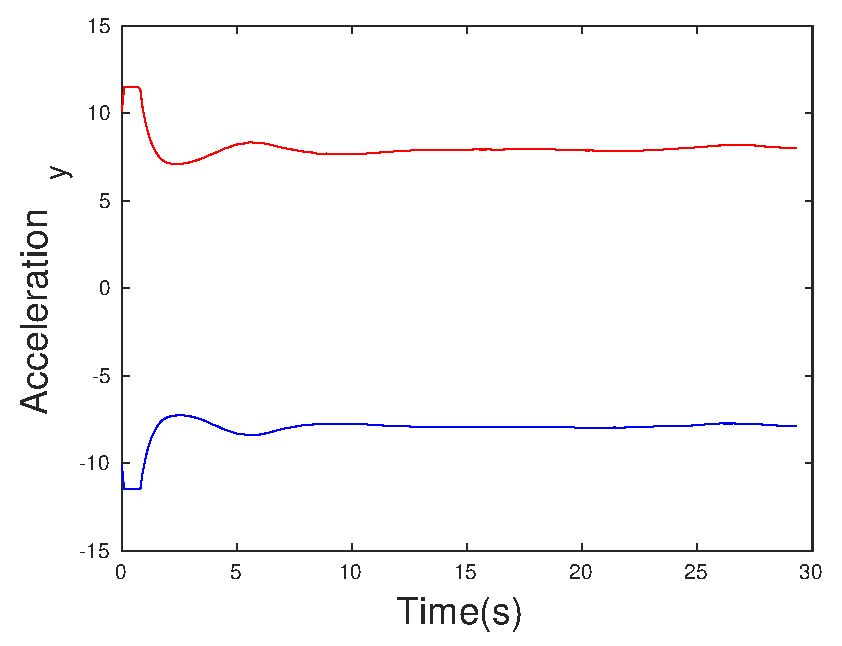
\includegraphics[width=\linewidth]{figures/Frad/s3pmSMAcceleration_y}
\end{subfigure}
\caption{Estimation using Point Mass Model}
\end{figure}

\clearpage
\subsubsection{Segment Minimization using P-Radius}
\FloatBarrier
\begin{figure}[h]
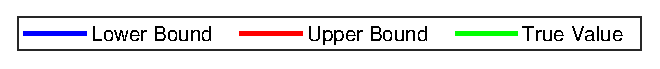
\includegraphics[scale=0.8]{figures/legend}\\\\
\begin{subfigure}{.5\linewidth}
\centering
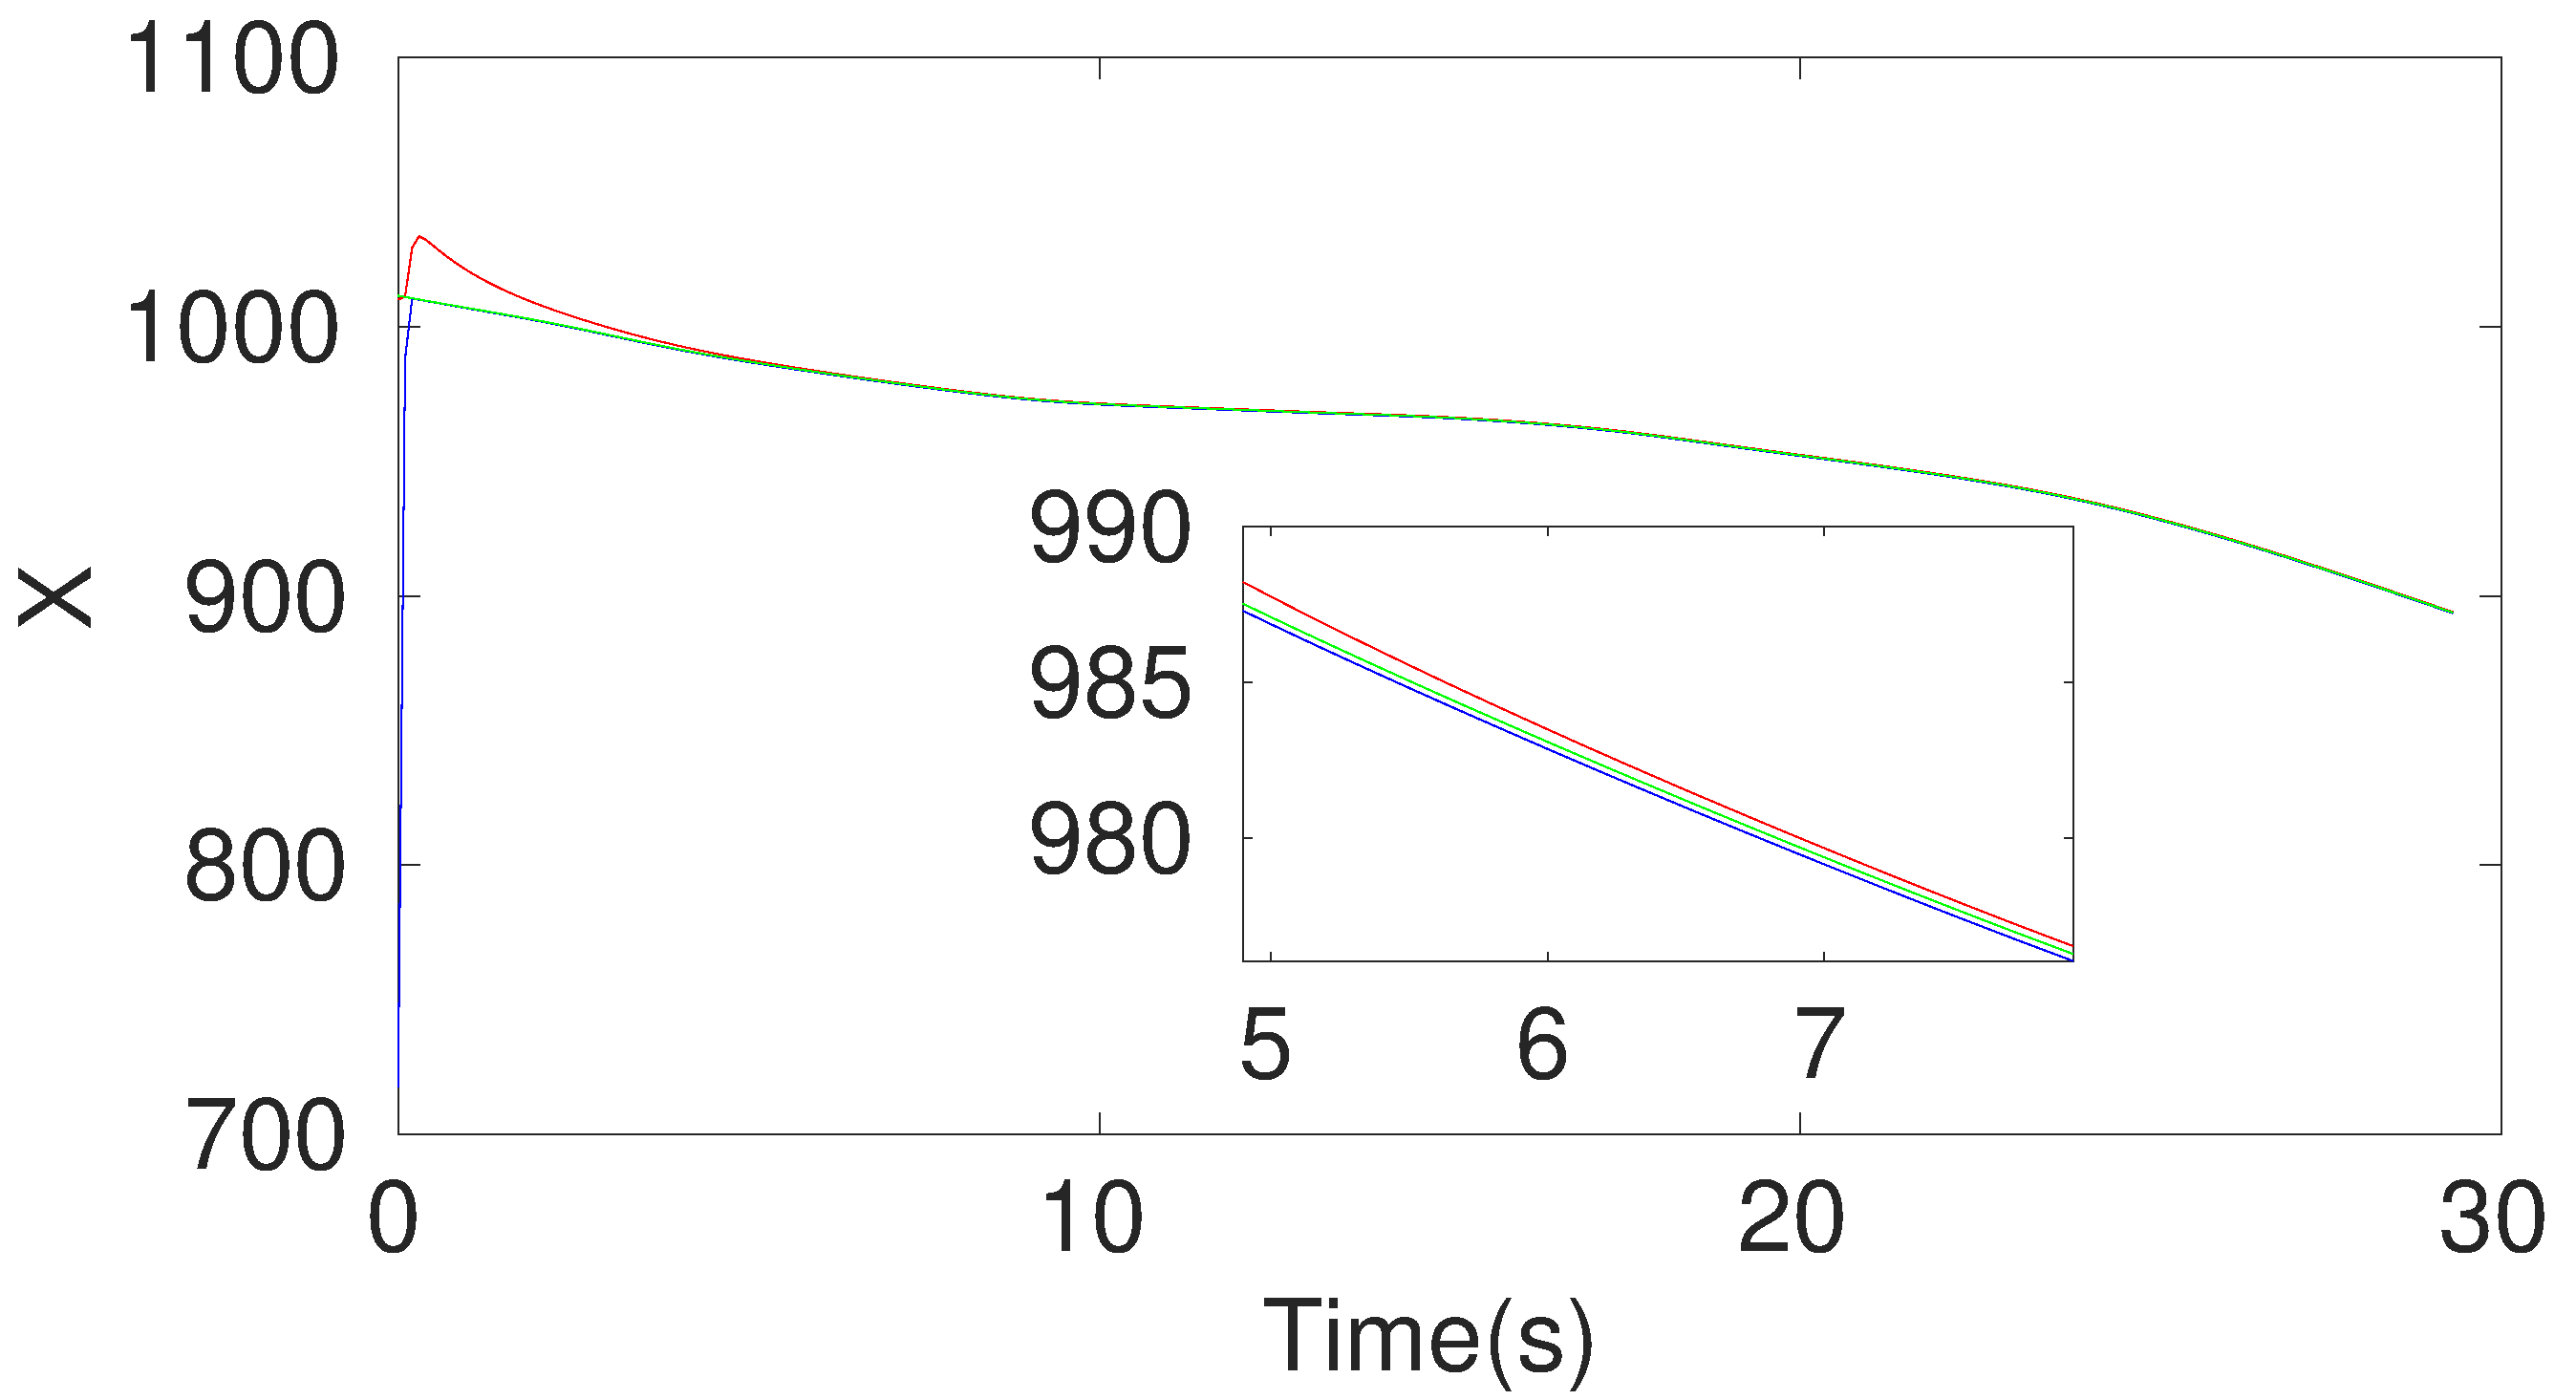
\includegraphics[width=\linewidth]{figures/Prad/s3cvpradX}
\end{subfigure}
\begin{subfigure}{.5\linewidth}
\centering
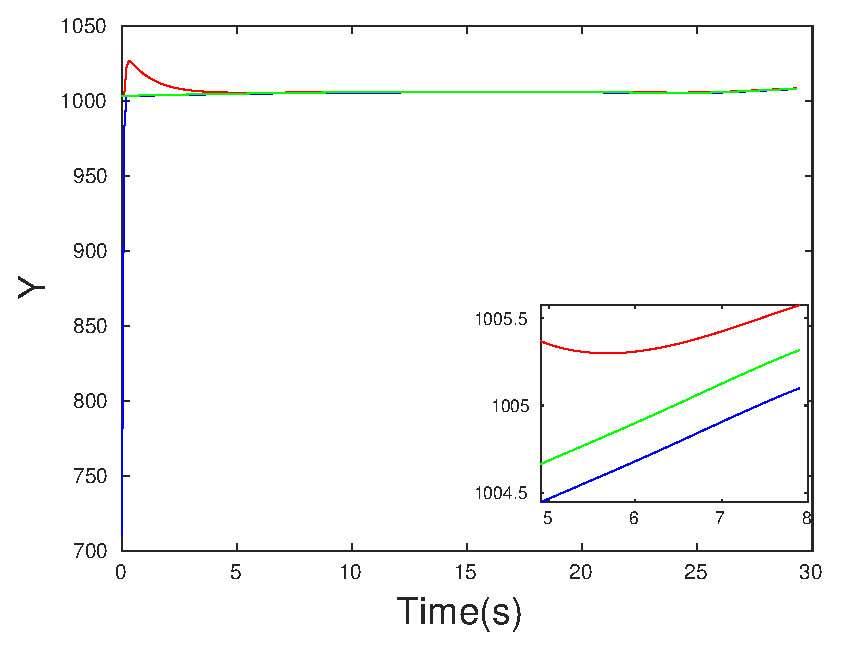
\includegraphics[width=\linewidth]{figures/Prad/s3cvpradY}
\end{subfigure}
\begin{subfigure}{.5\linewidth}
\centering
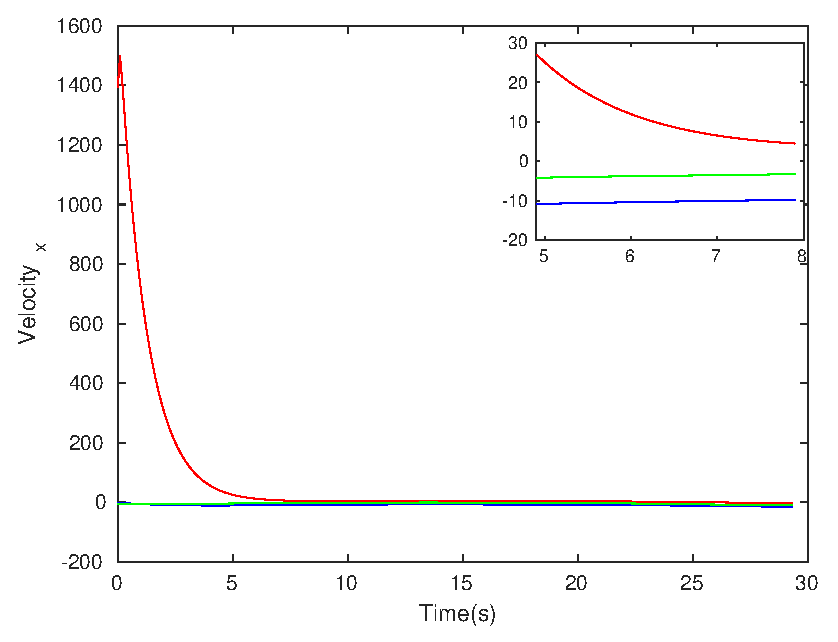
\includegraphics[width=\linewidth]{figures/Prad/s3cvpradVelocity_x}
\end{subfigure}
\begin{subfigure}{.5\linewidth}
\centering
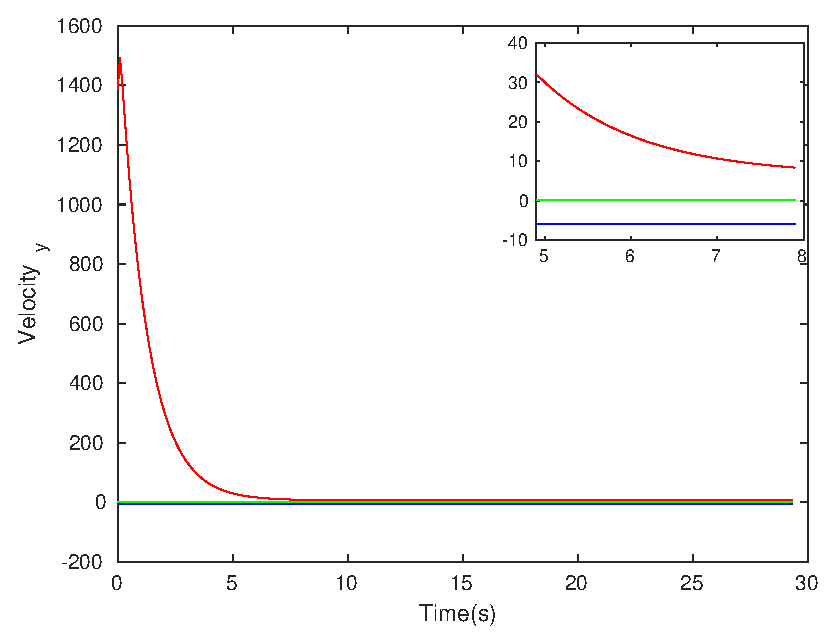
\includegraphics[width=\linewidth]{figures/Prad/s3cvpradVelocity_y}
\end{subfigure}
\caption{Estimation using Constant Velocity}
\end{figure}

\begin{figure}[h]
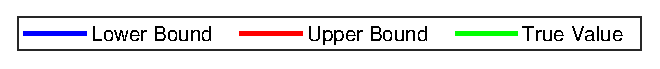
\includegraphics[scale=0.8]{figures/legend}\\\\
\begin{subfigure}{.5\linewidth}
\centering
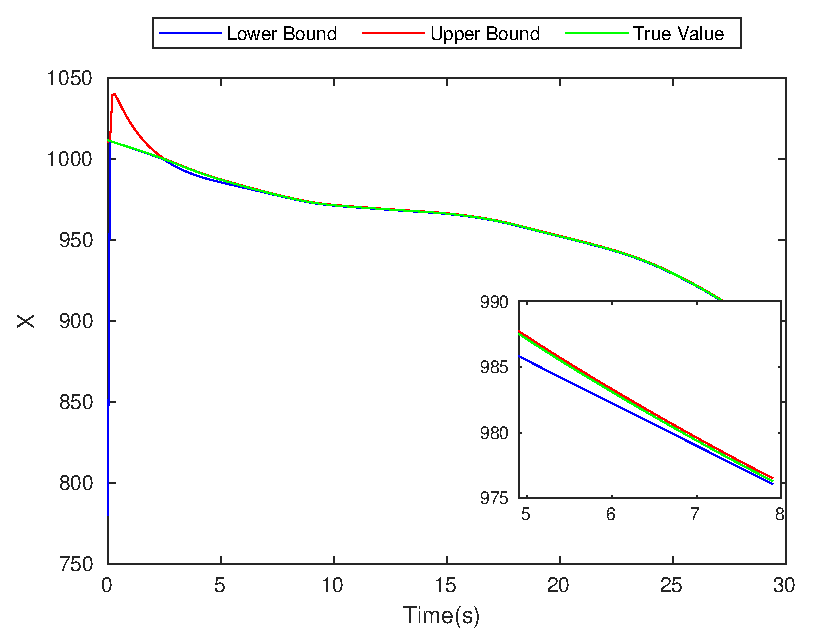
\includegraphics[width=\linewidth]{figures/Prad/s3capradX}
\end{subfigure}
\begin{subfigure}{.5\linewidth}
\centering
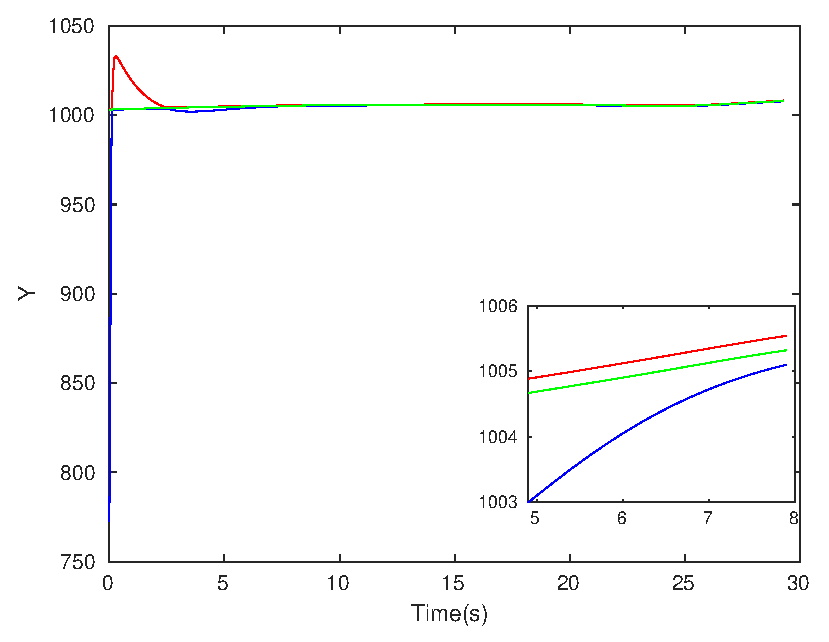
\includegraphics[width=\linewidth]{figures/Prad/s3capradY}
\end{subfigure}
\begin{subfigure}{.5\linewidth}
\centering
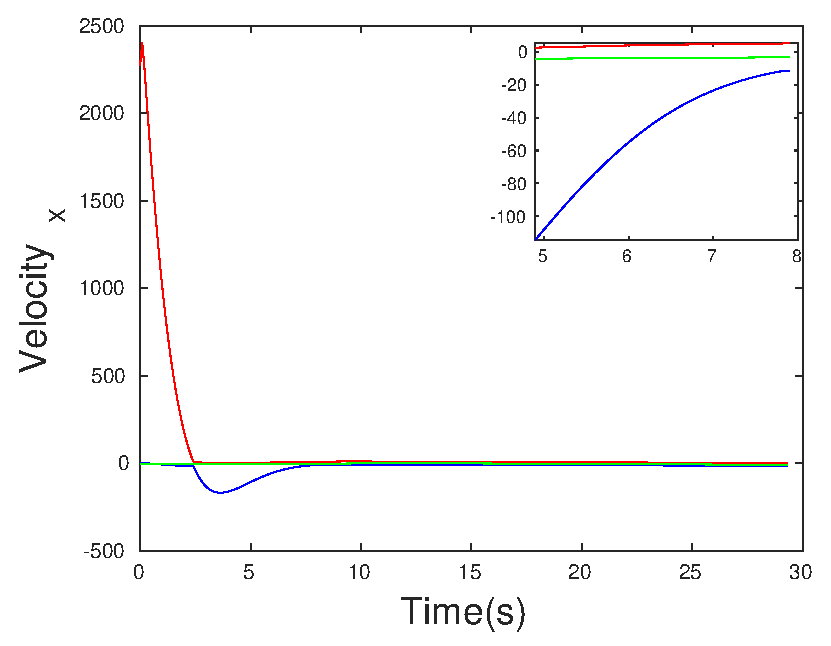
\includegraphics[width=\linewidth]{figures/Prad/s3capradVelocity_x}
\end{subfigure}
\begin{subfigure}{.5\linewidth}
\centering
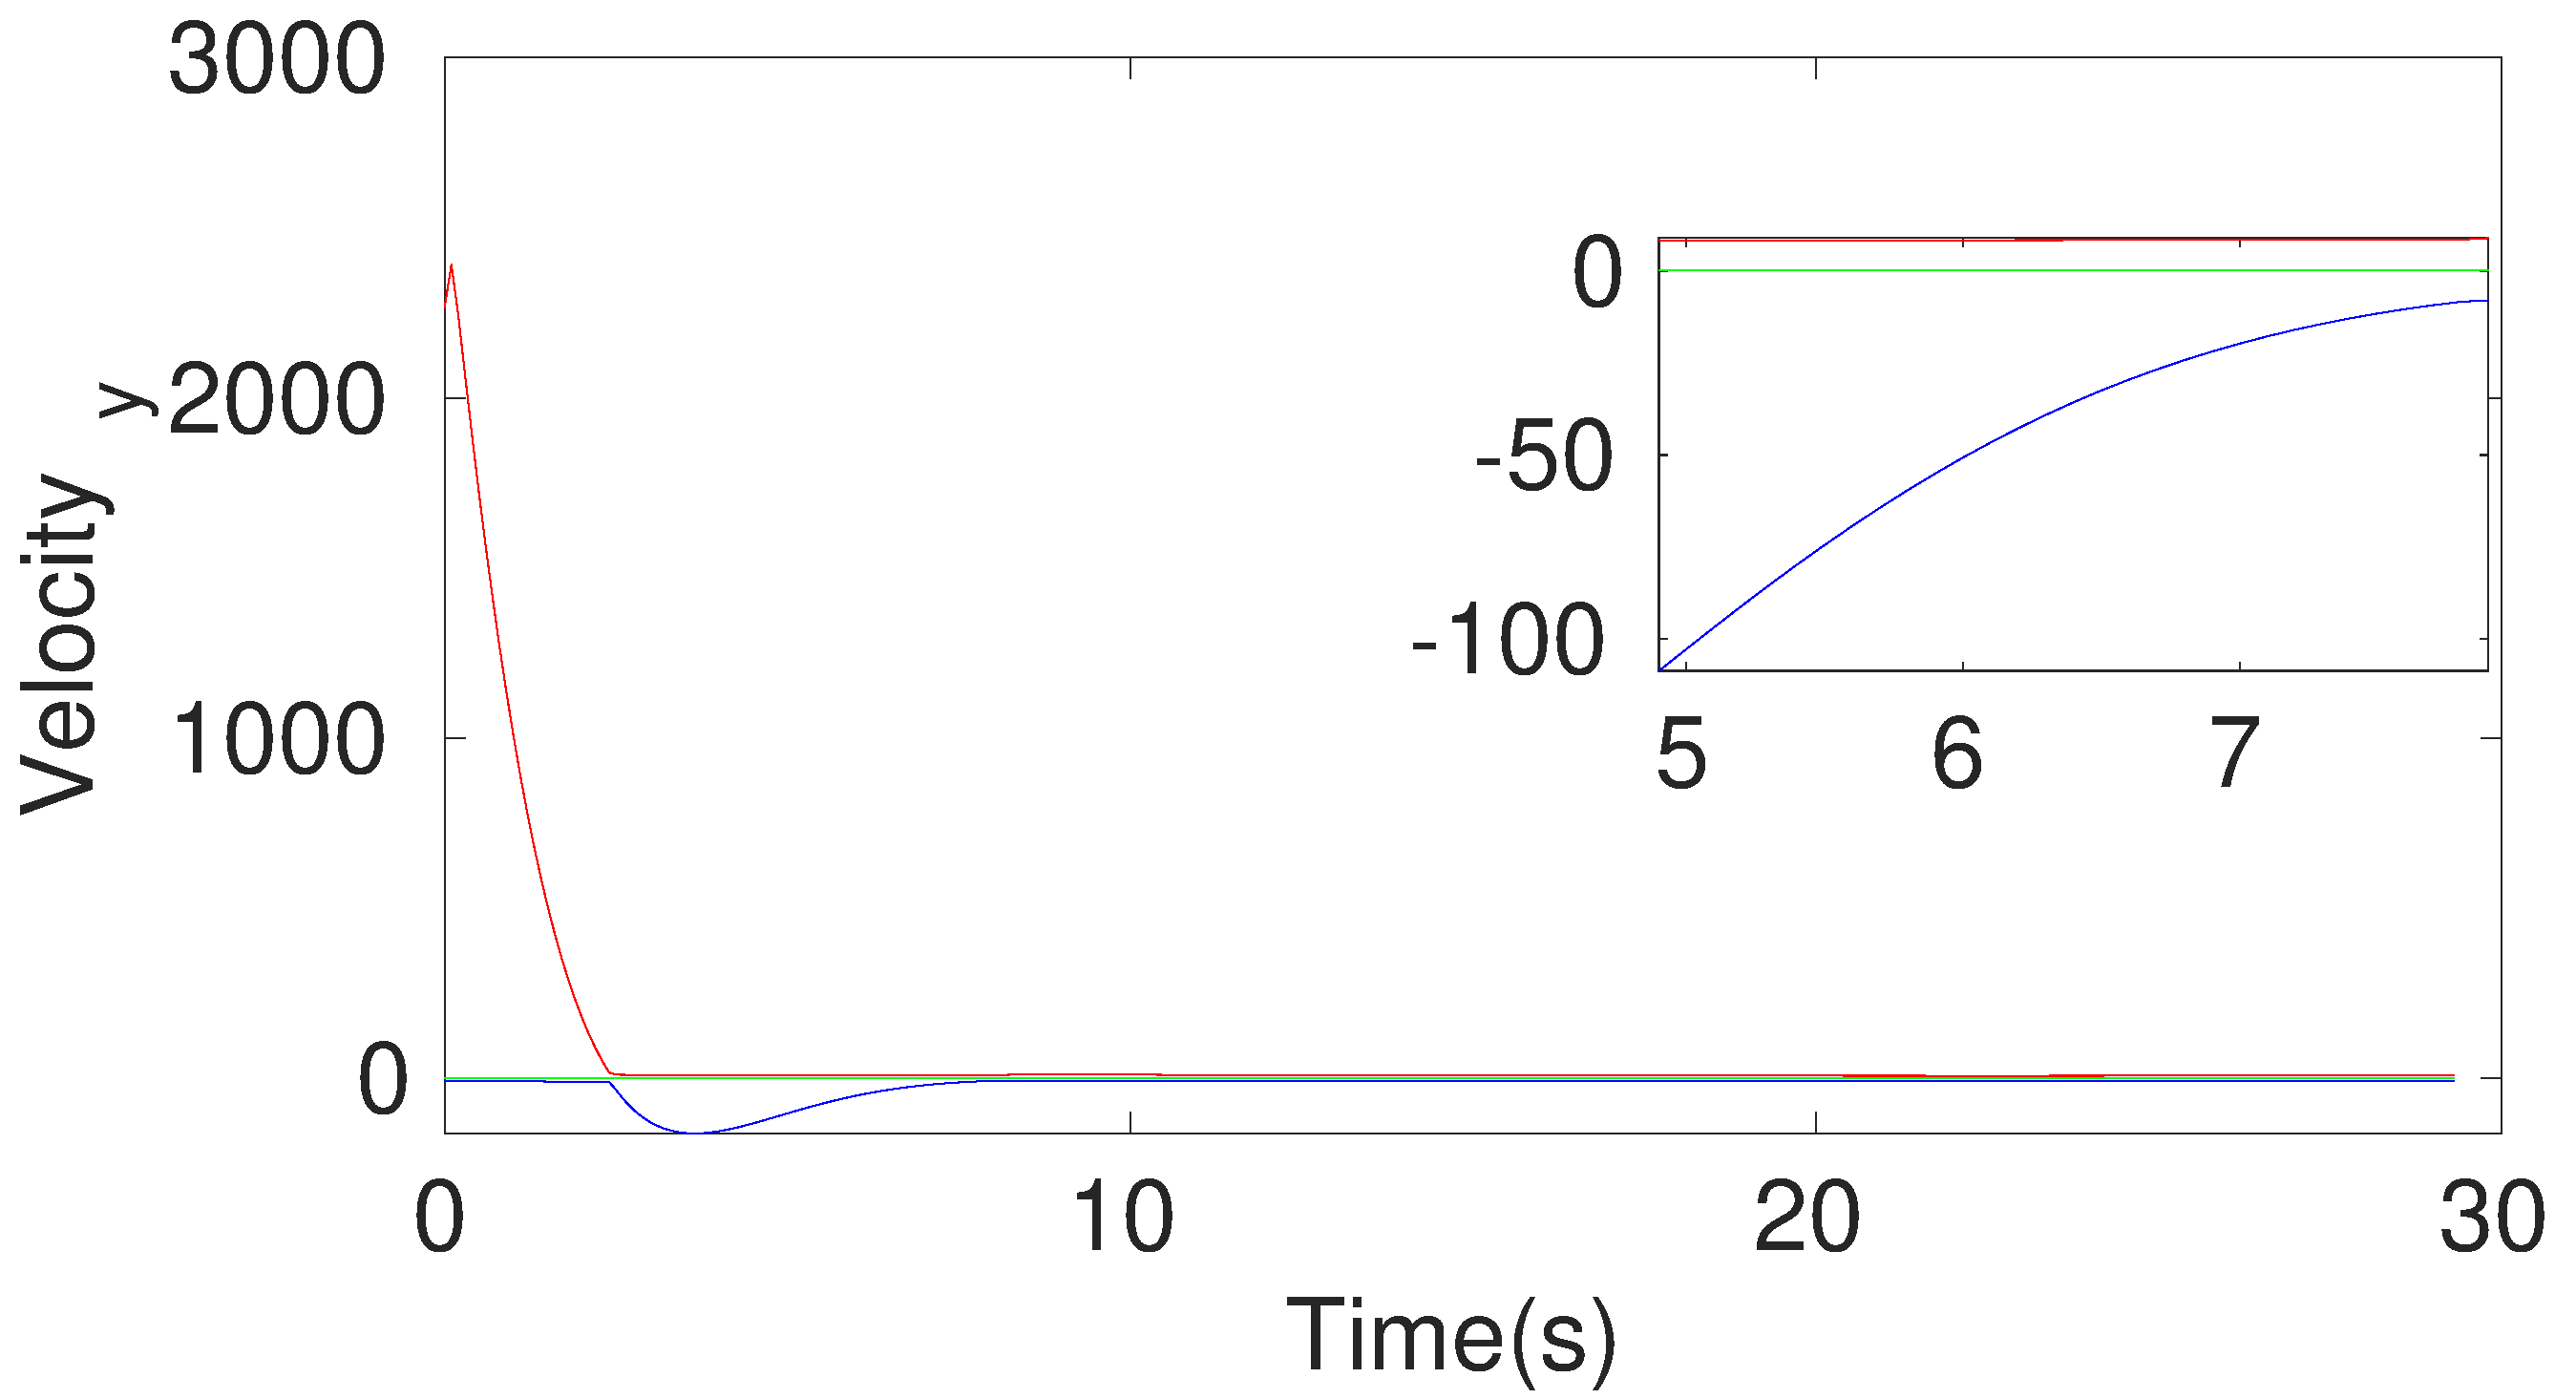
\includegraphics[width=\linewidth]{figures/Prad/s3capradVelocity_y}
\end{subfigure}
\begin{subfigure}{.5\linewidth}
\centering
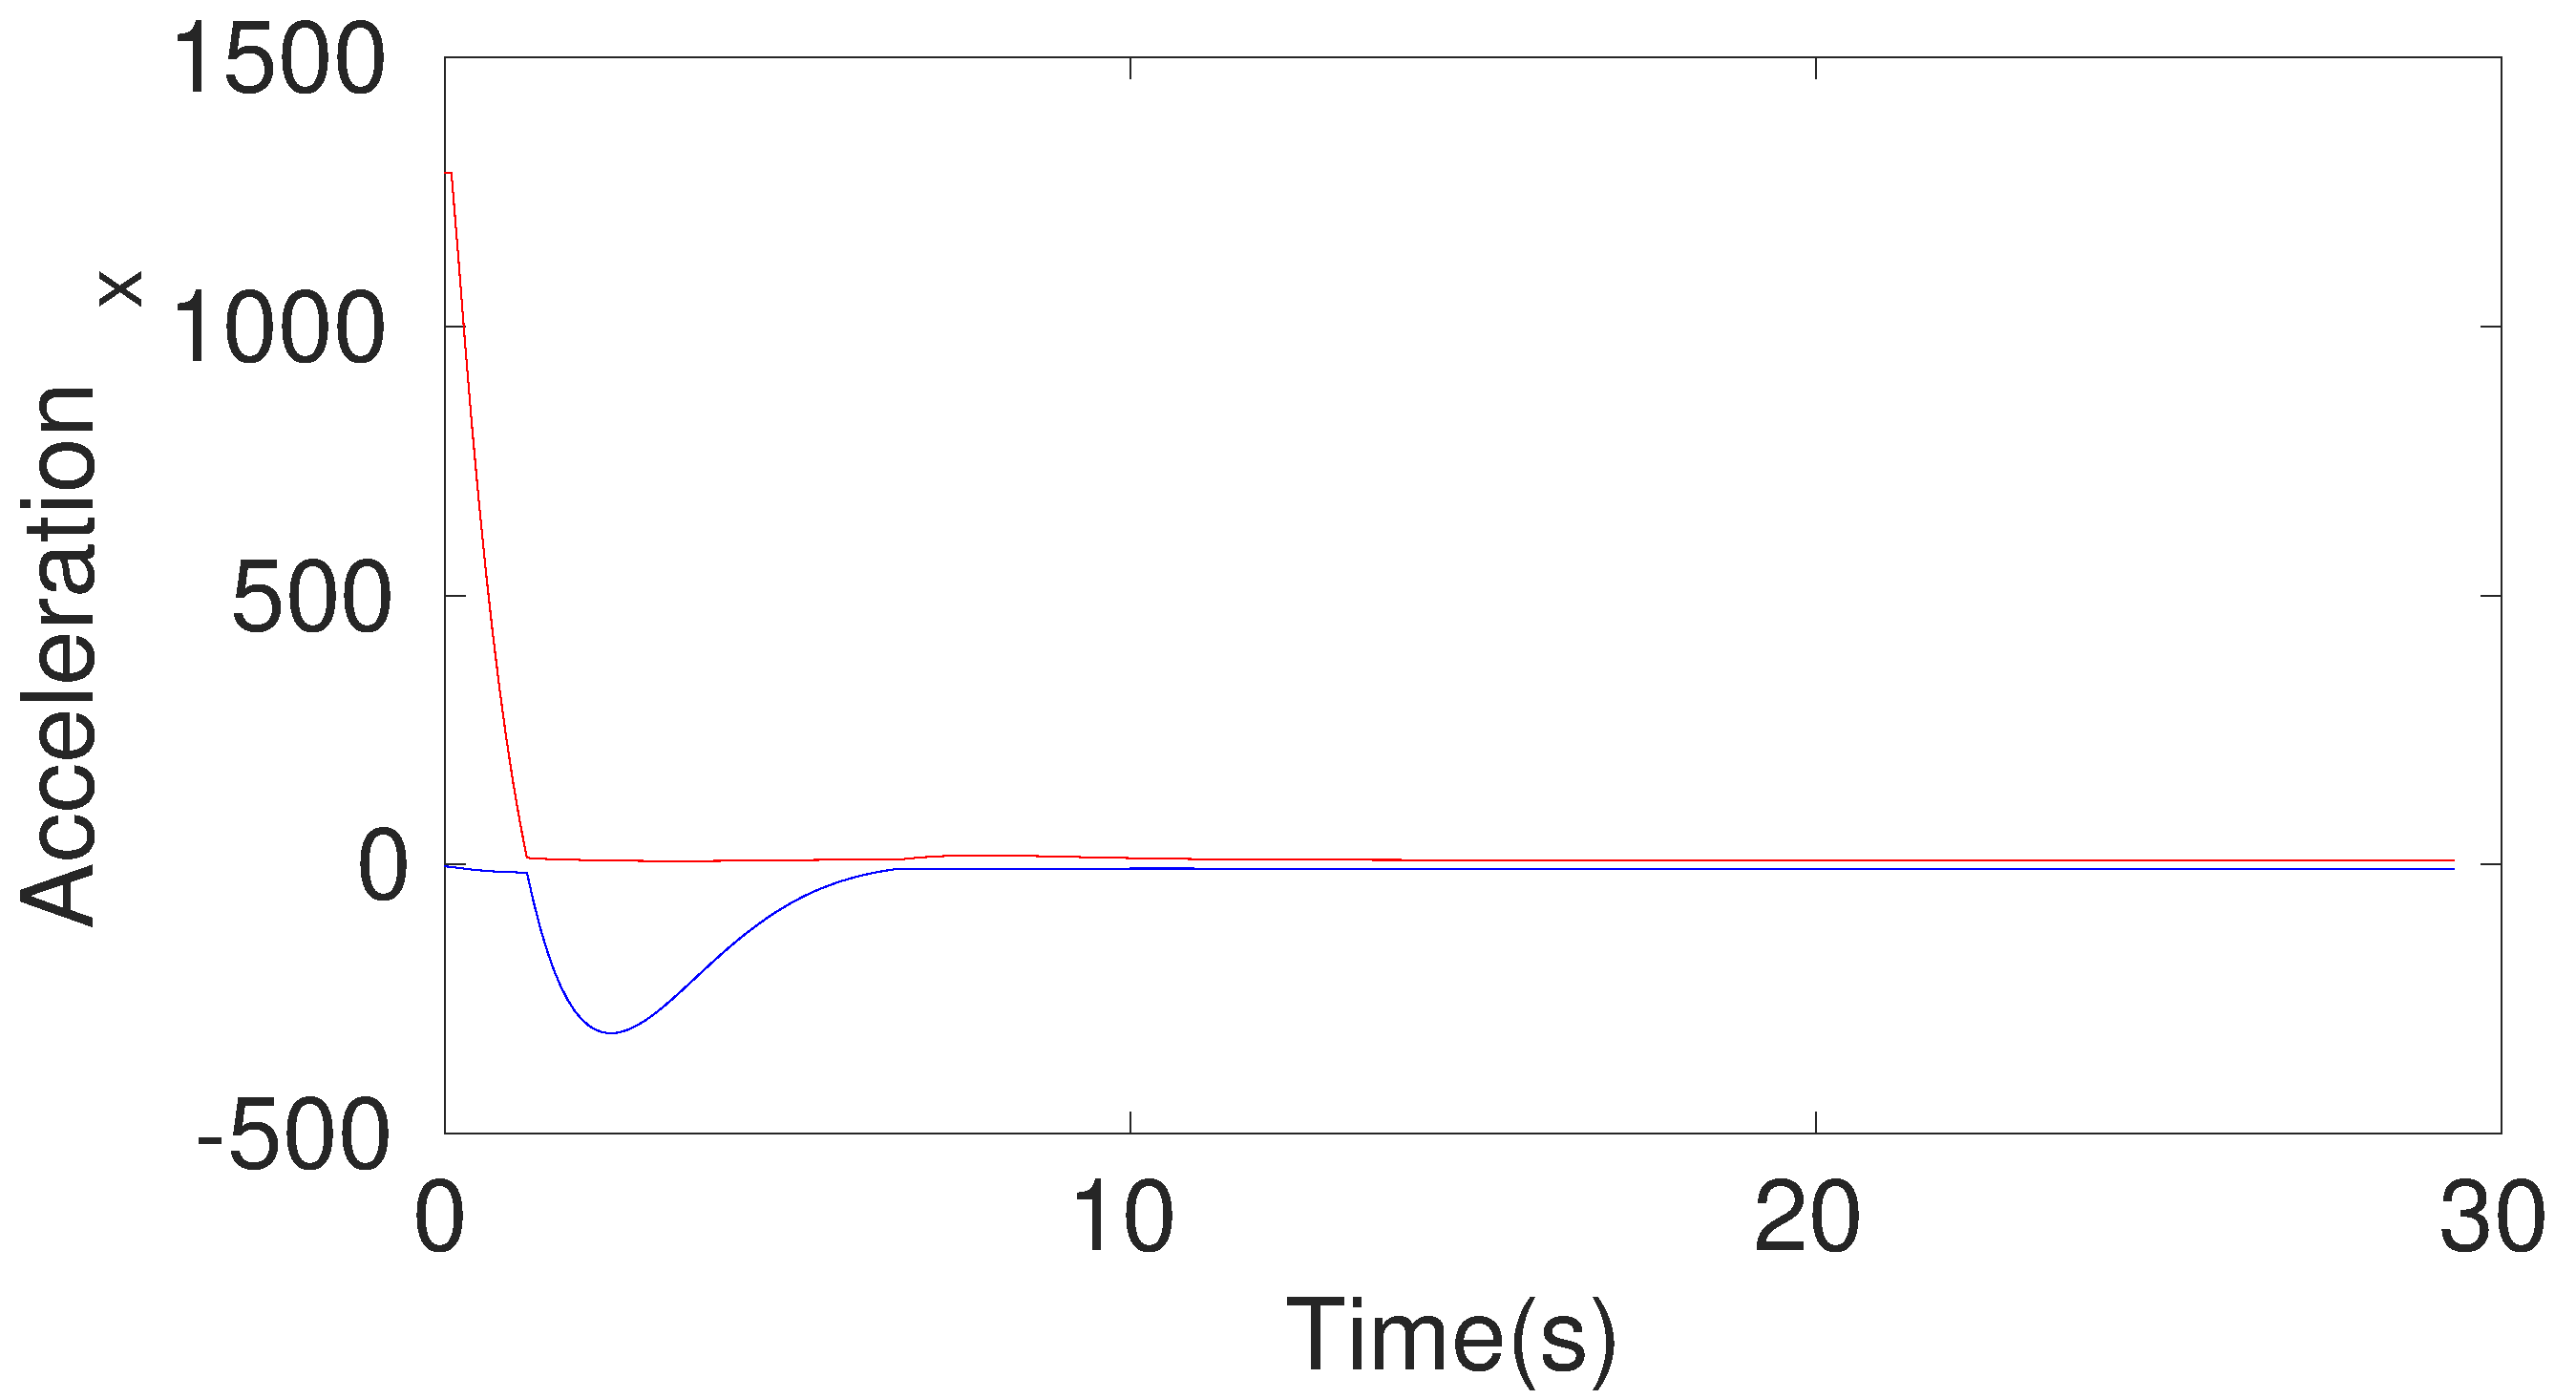
\includegraphics[width=\linewidth]{figures/Prad/s3capradAcceleration_x}
\end{subfigure}
\begin{subfigure}{.5\linewidth}
\centering
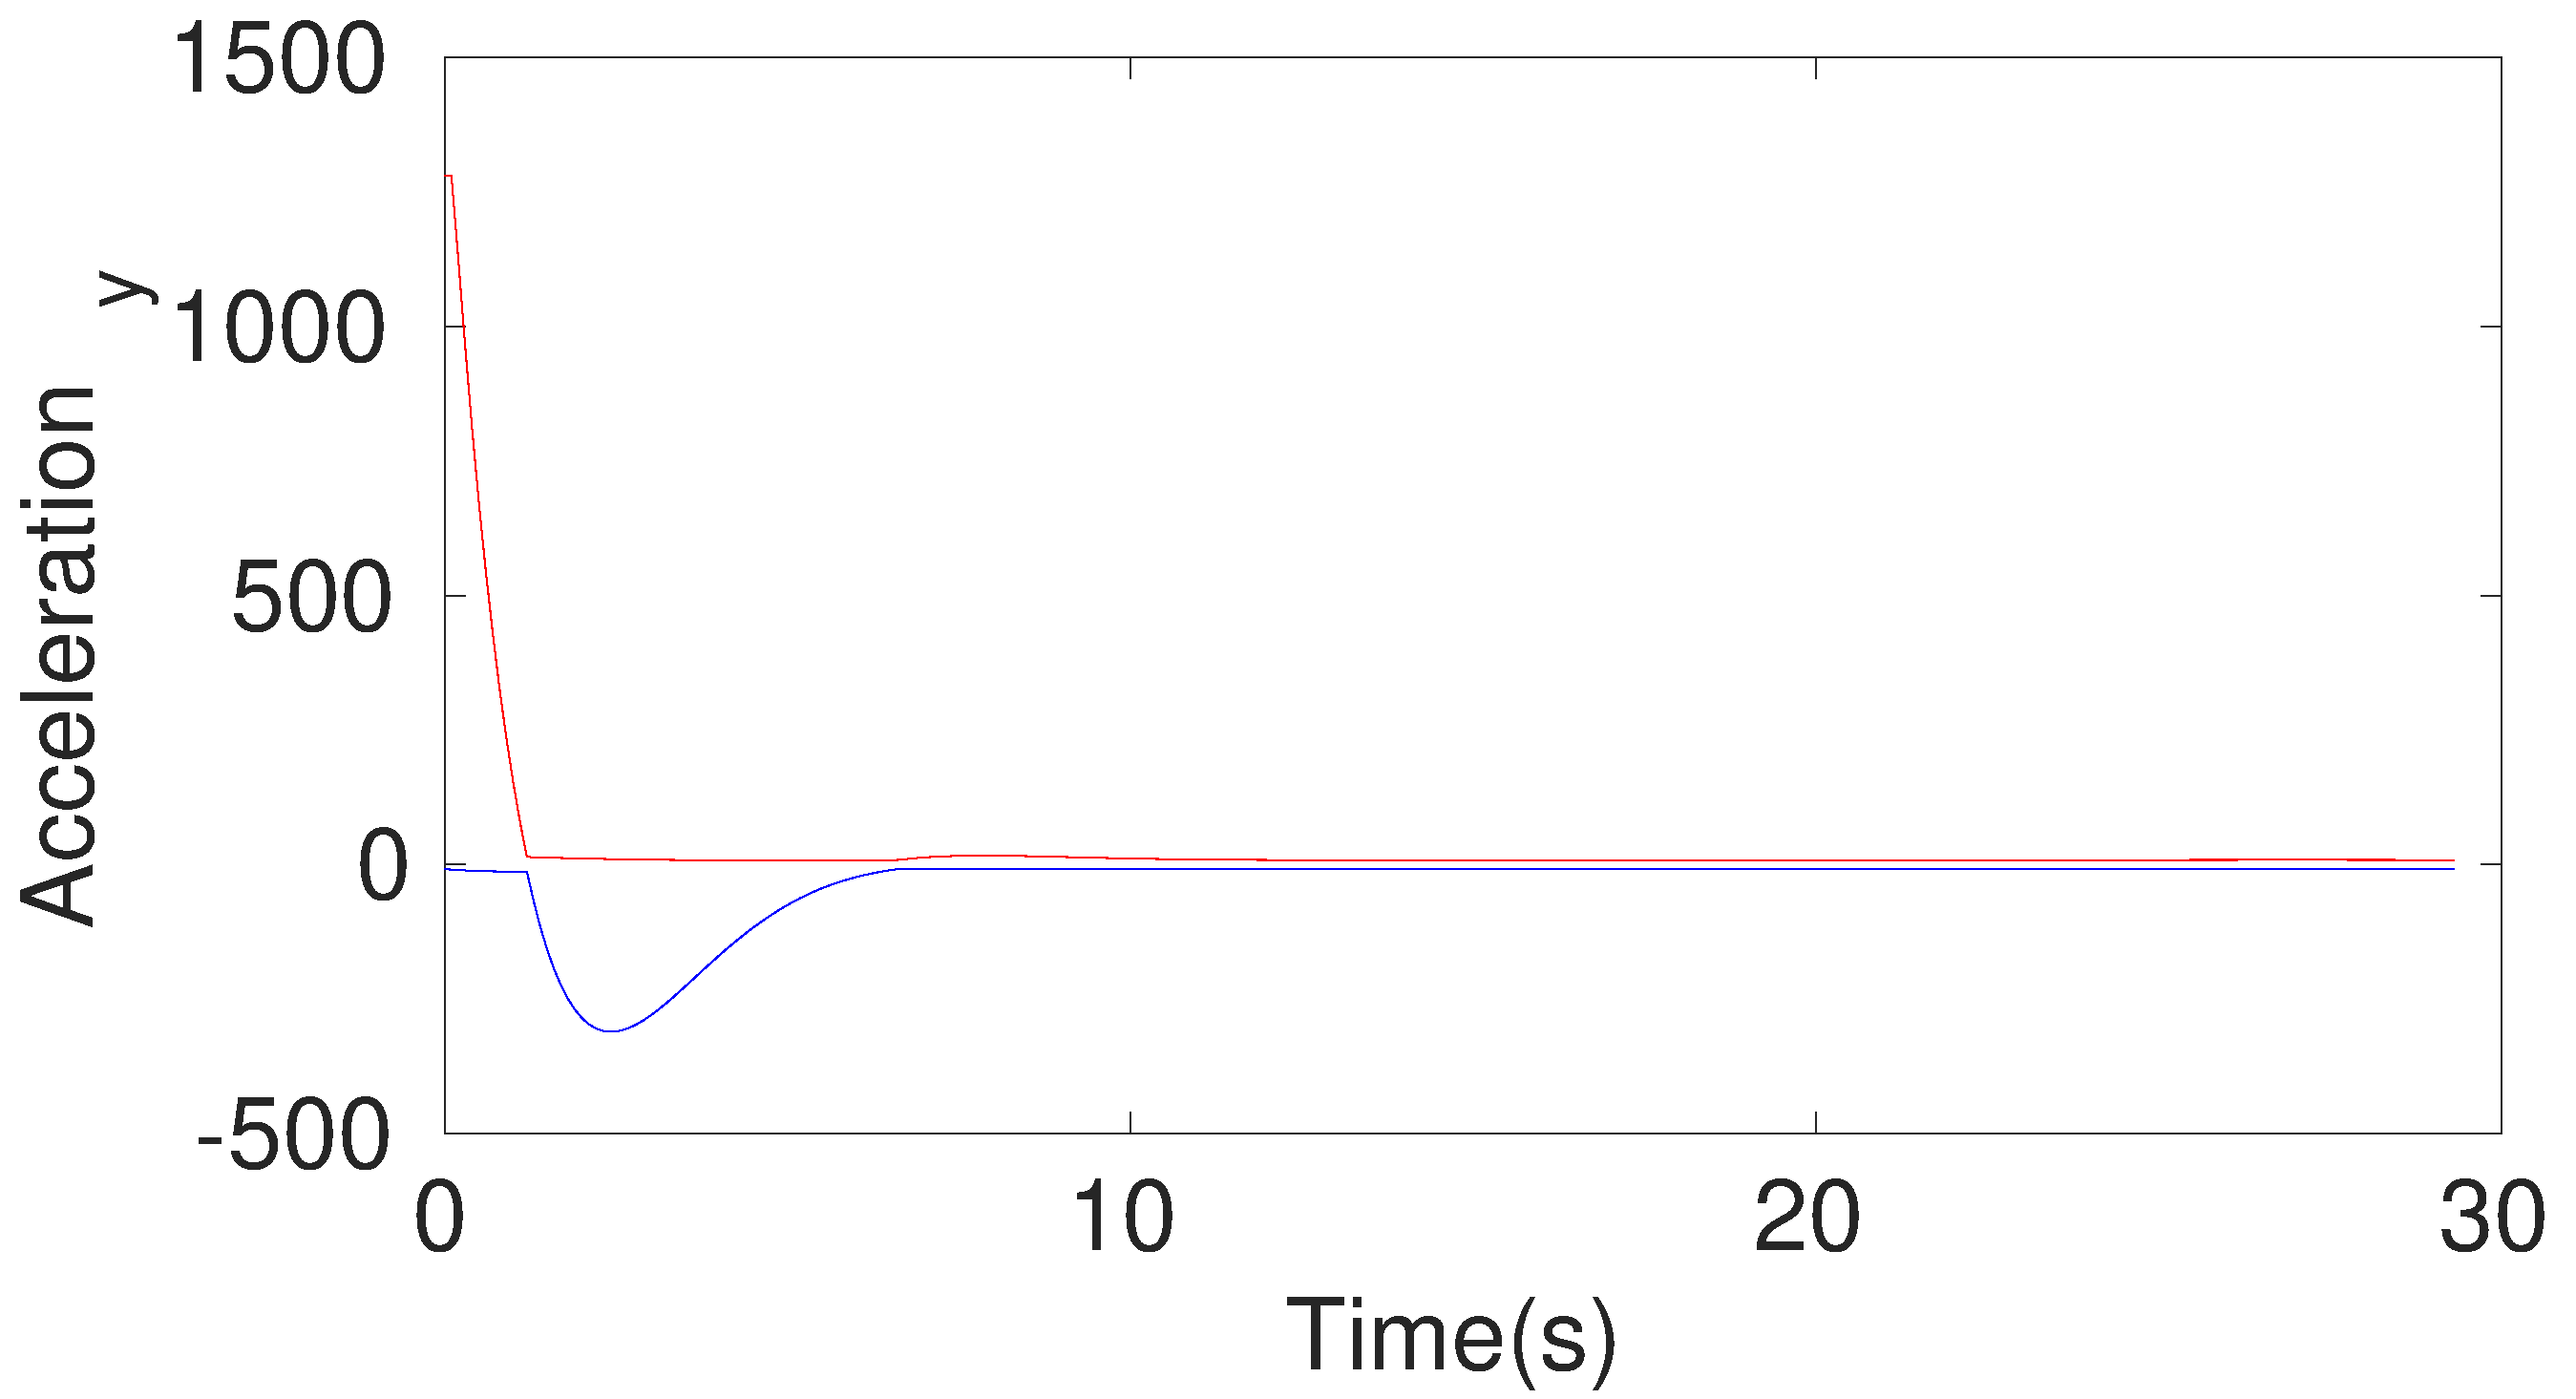
\includegraphics[width=\linewidth]{figures/Prad/s3capradAcceleration_y}
\end{subfigure}
\caption{Estimation using Constant Acceleration}
\end{figure}

\begin{figure}[h]
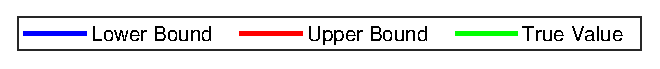
\includegraphics[scale=0.8]{figures/legend}\\\\
\begin{subfigure}{.5\linewidth}
\centering
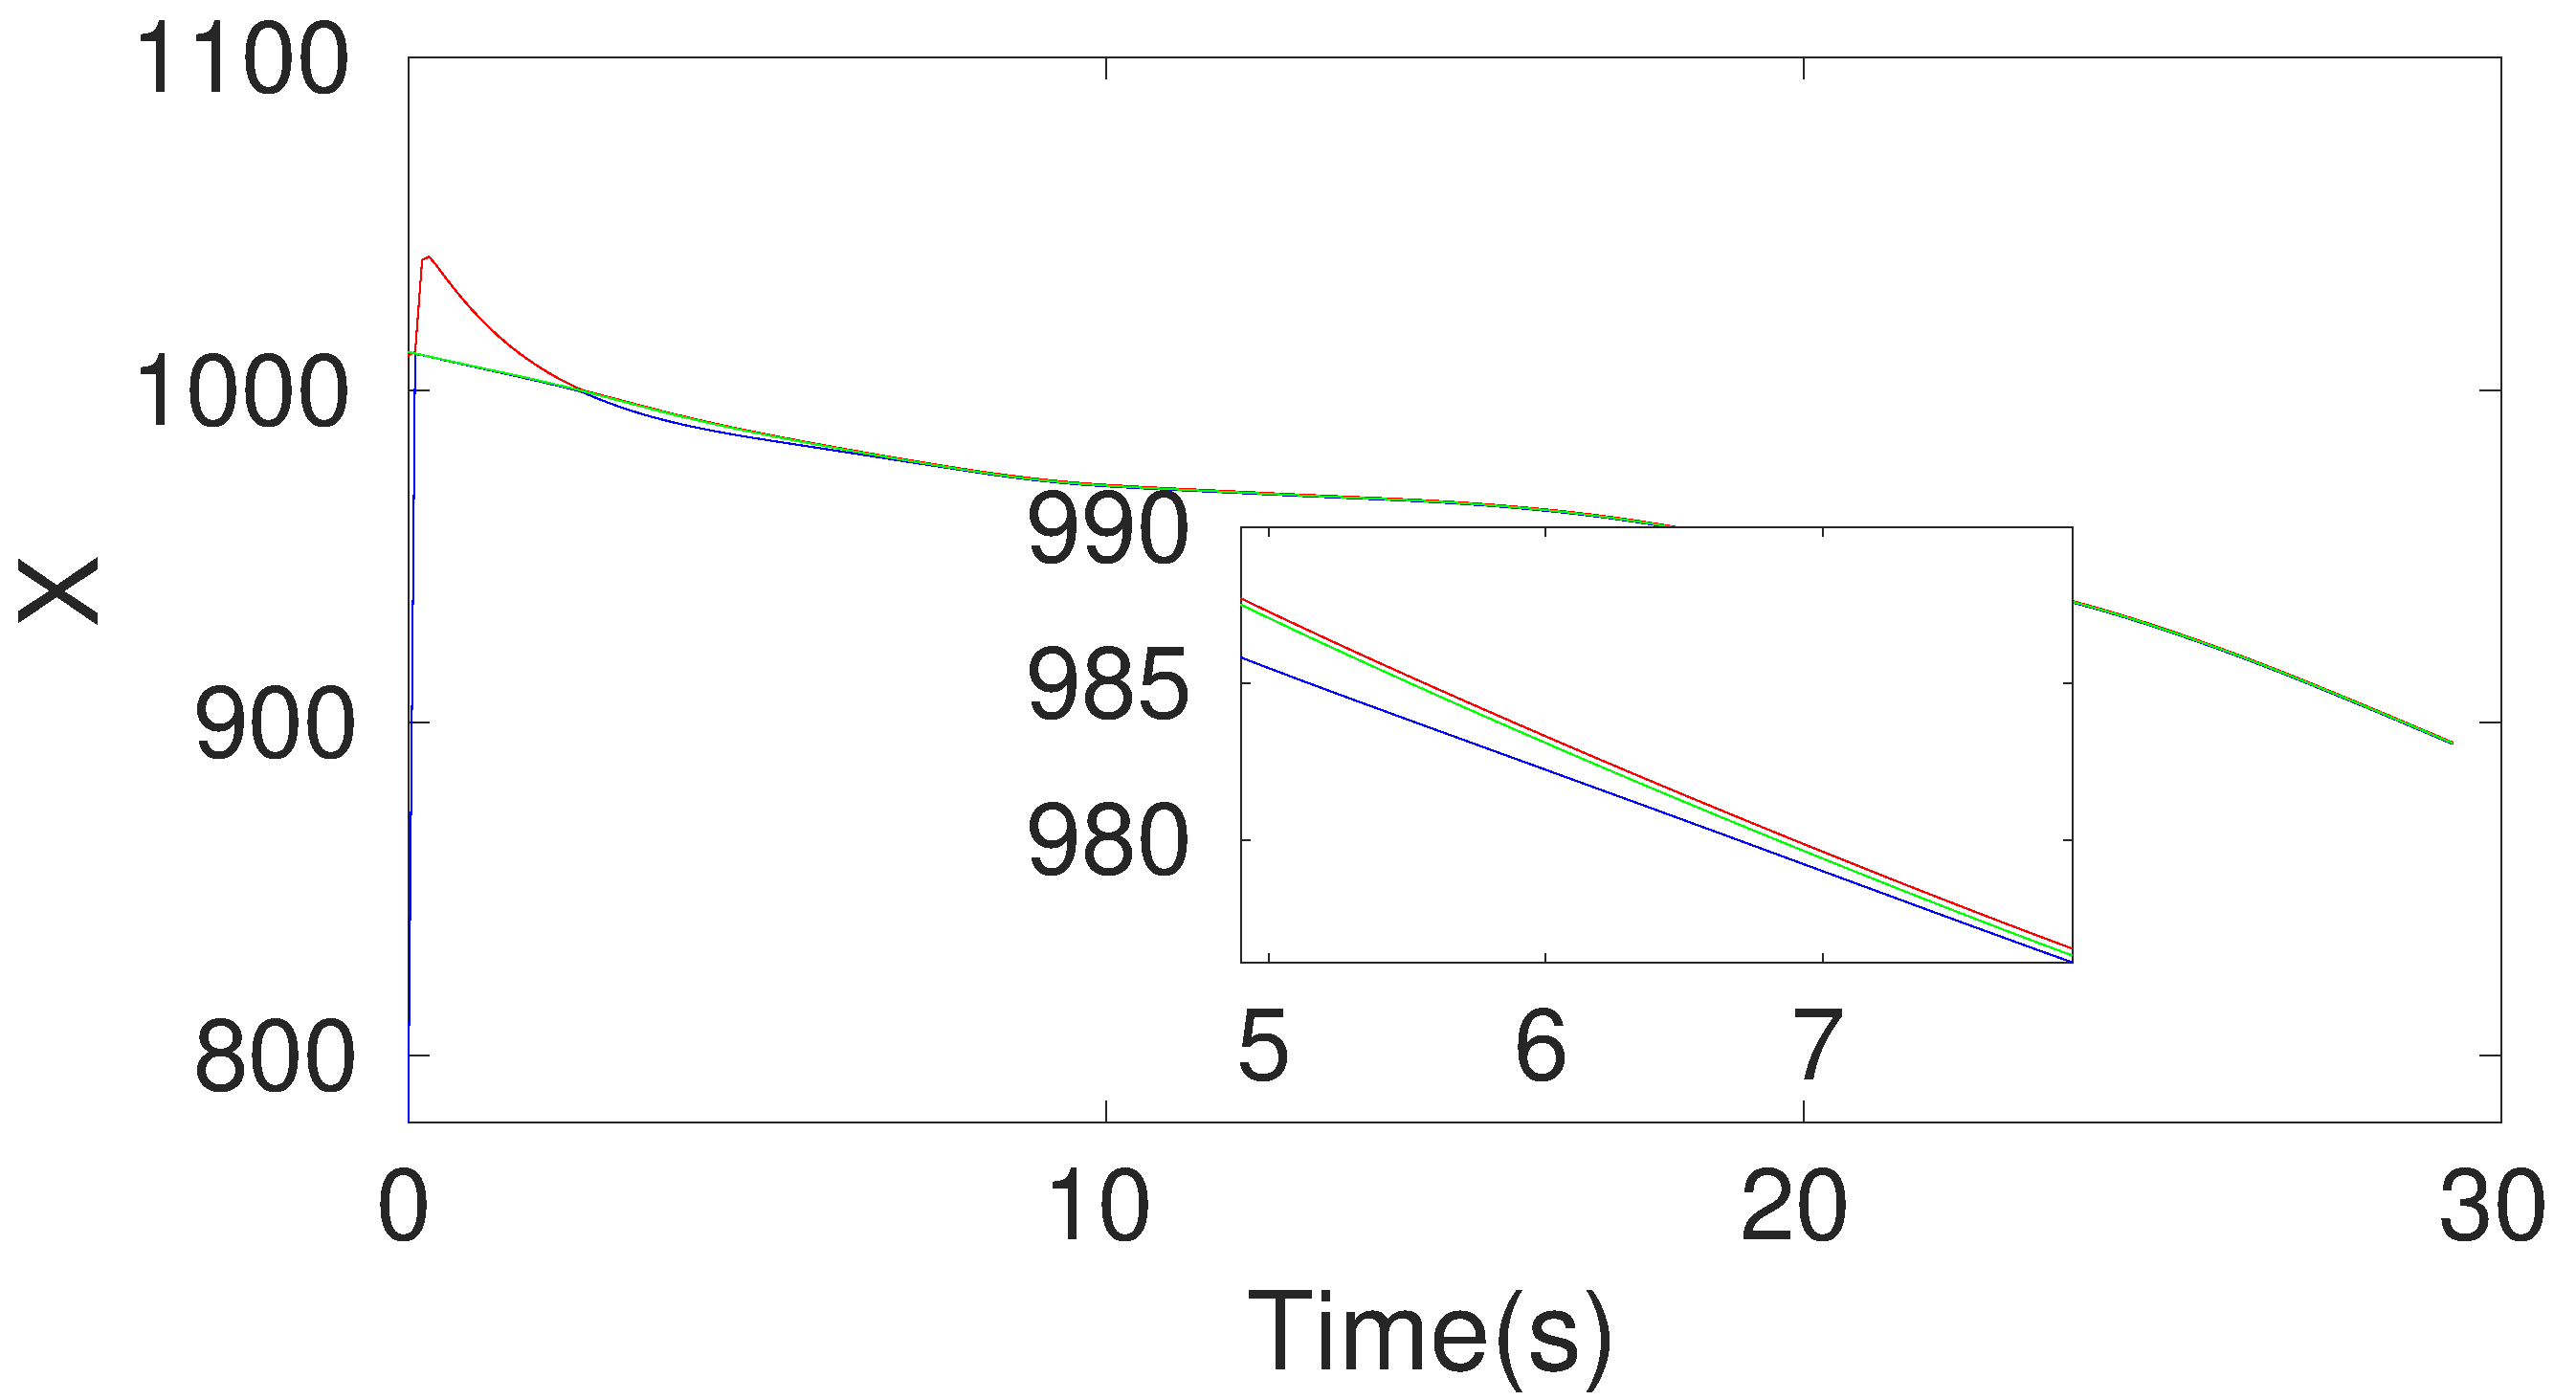
\includegraphics[width=\linewidth]{figures/Prad/s3pmpradX}
\end{subfigure}
\begin{subfigure}{.5\linewidth}
\centering
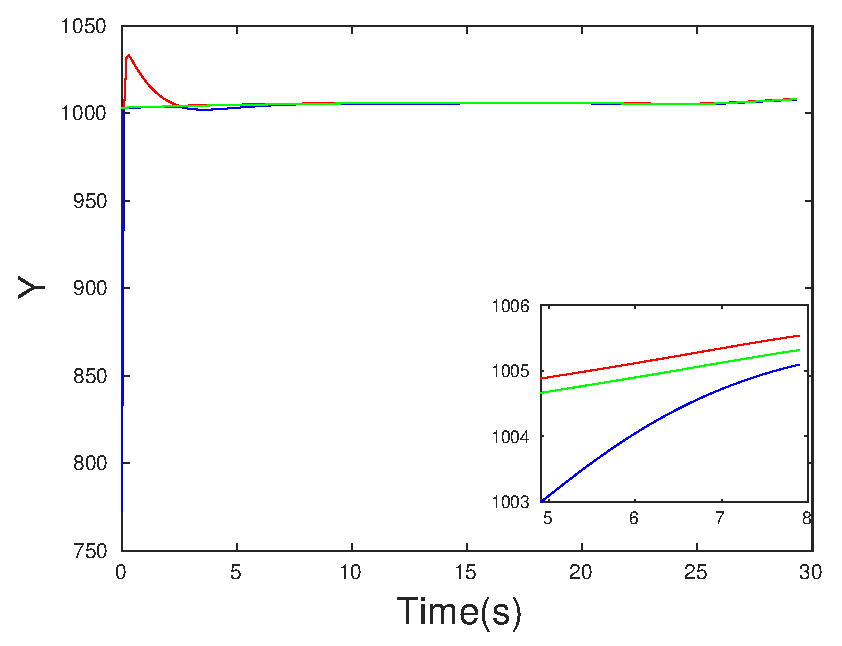
\includegraphics[width=\linewidth]{figures/Prad/s3pmpradY}
\end{subfigure}
\begin{subfigure}{.5\linewidth}
\centering
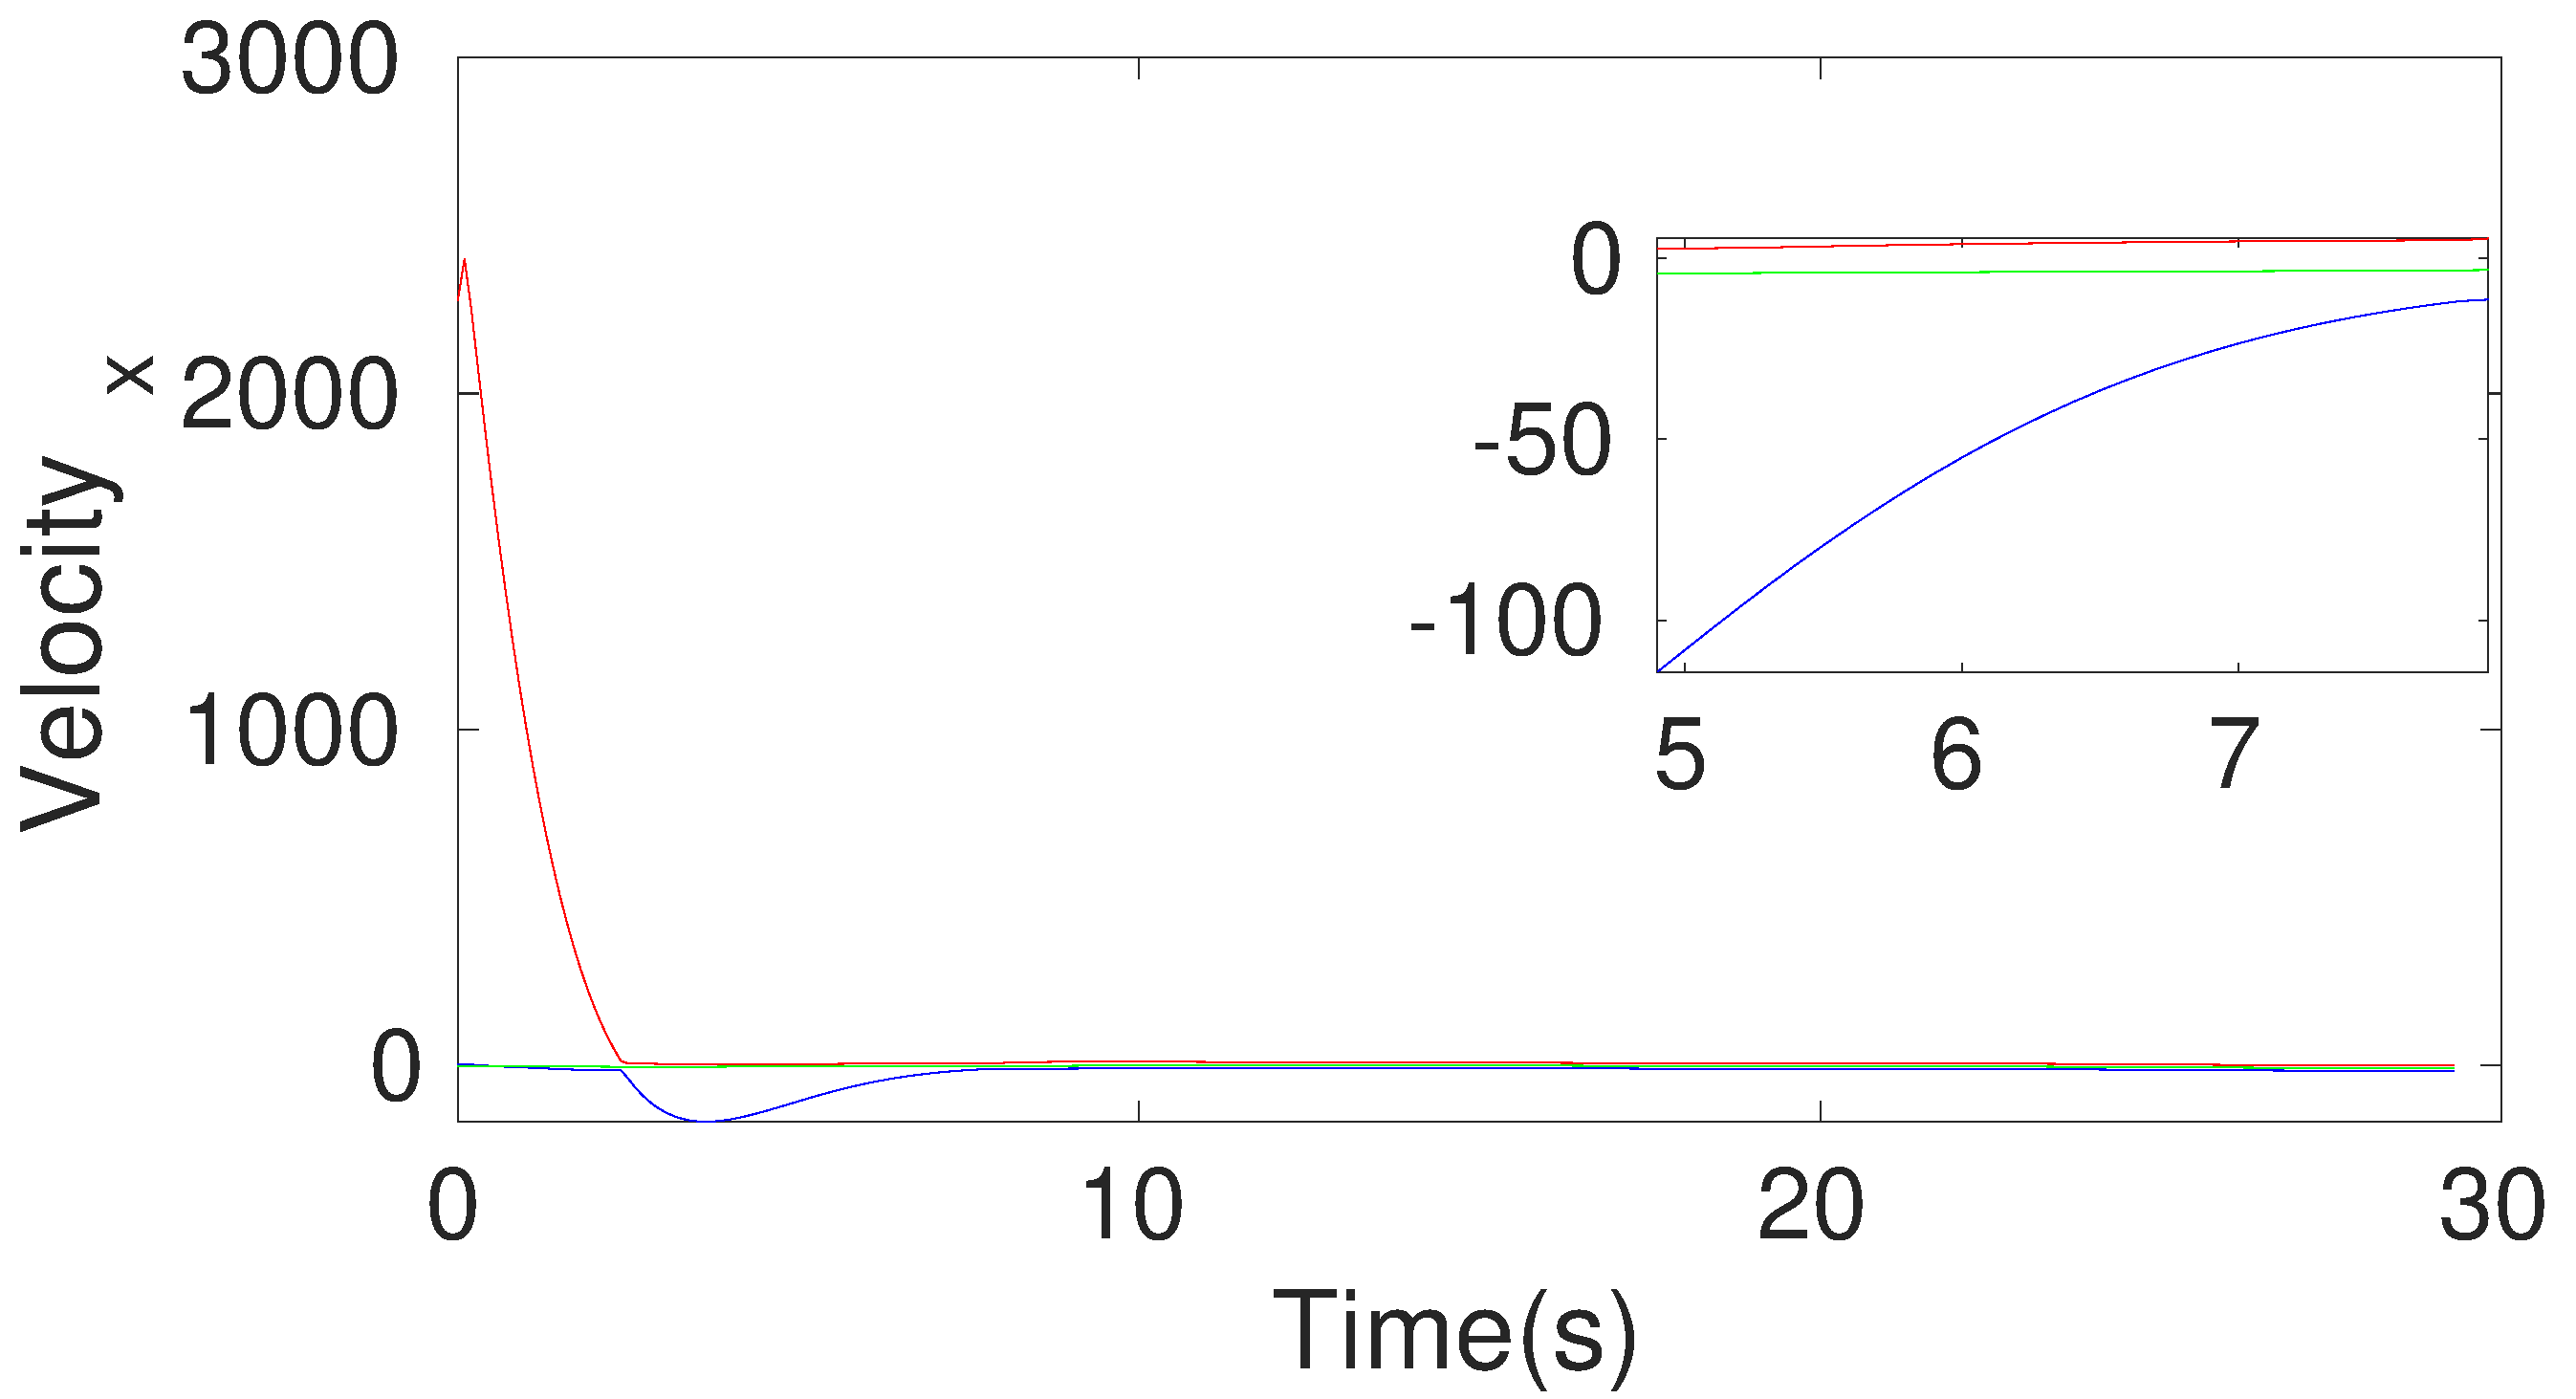
\includegraphics[width=\linewidth]{figures/Prad/s3pmpradVelocity_x}
\end{subfigure}
\begin{subfigure}{.5\linewidth}
\centering
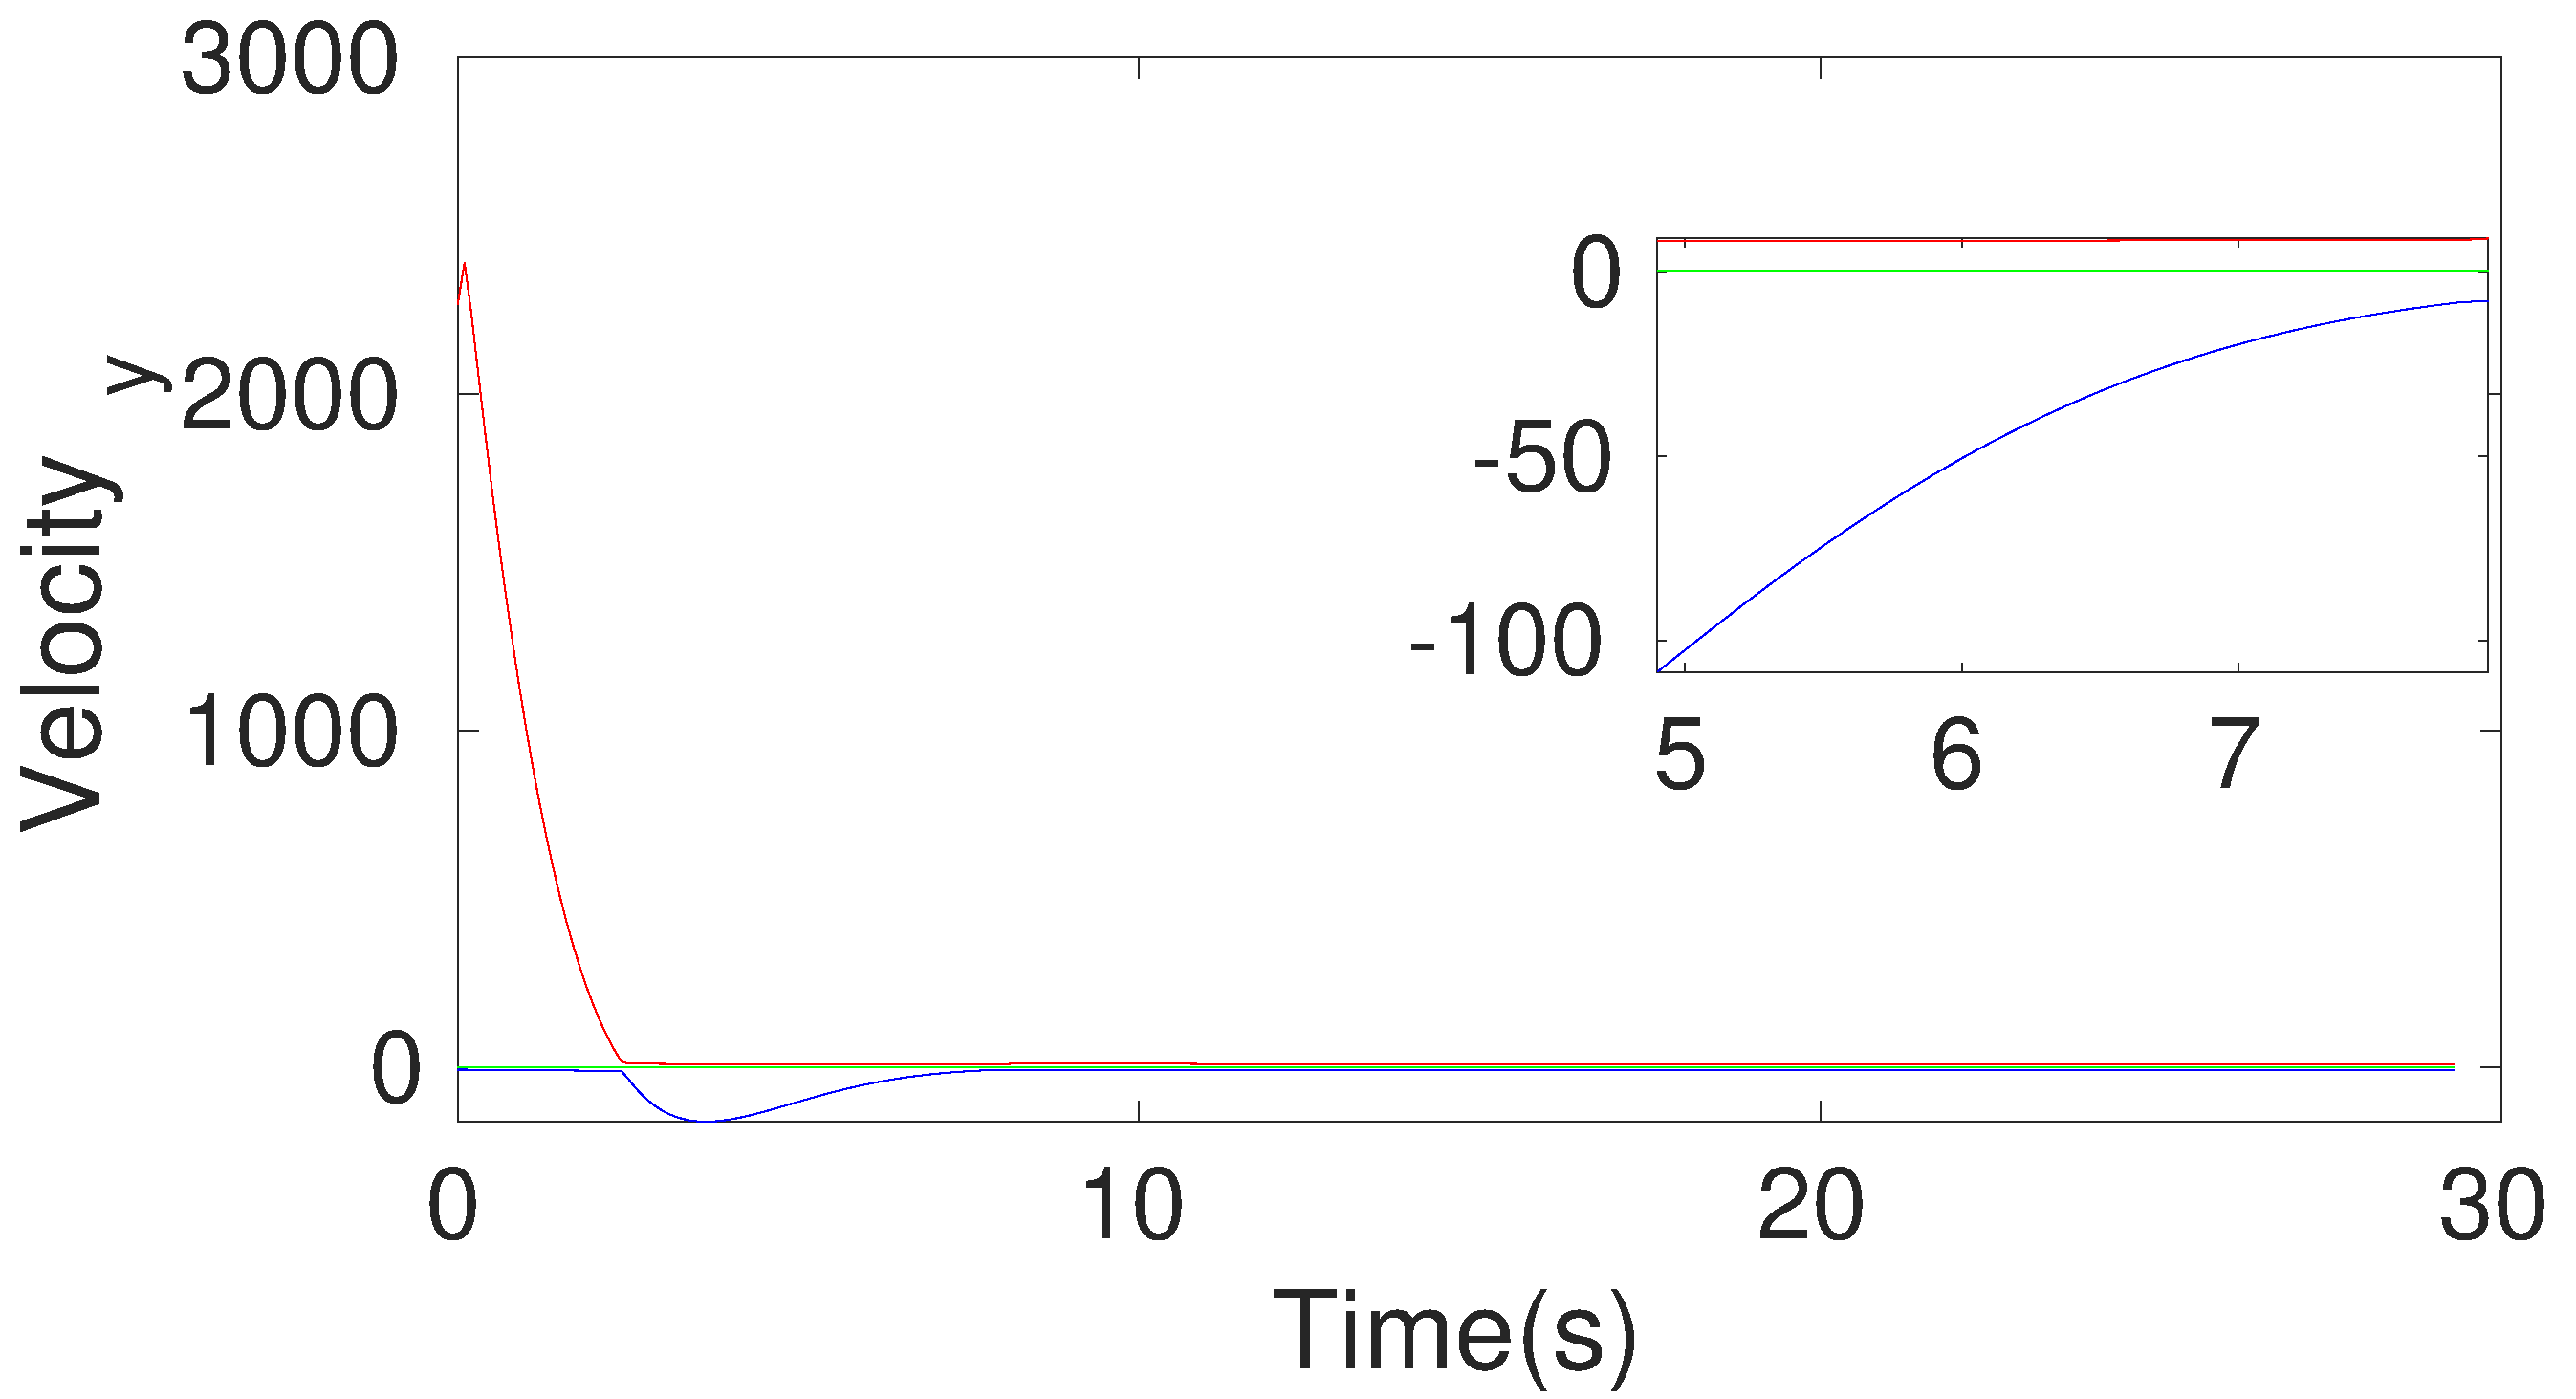
\includegraphics[width=\linewidth]{figures/Prad/s3pmpradVelocity_y}
\end{subfigure}
\begin{subfigure}{.5\linewidth}
\centering
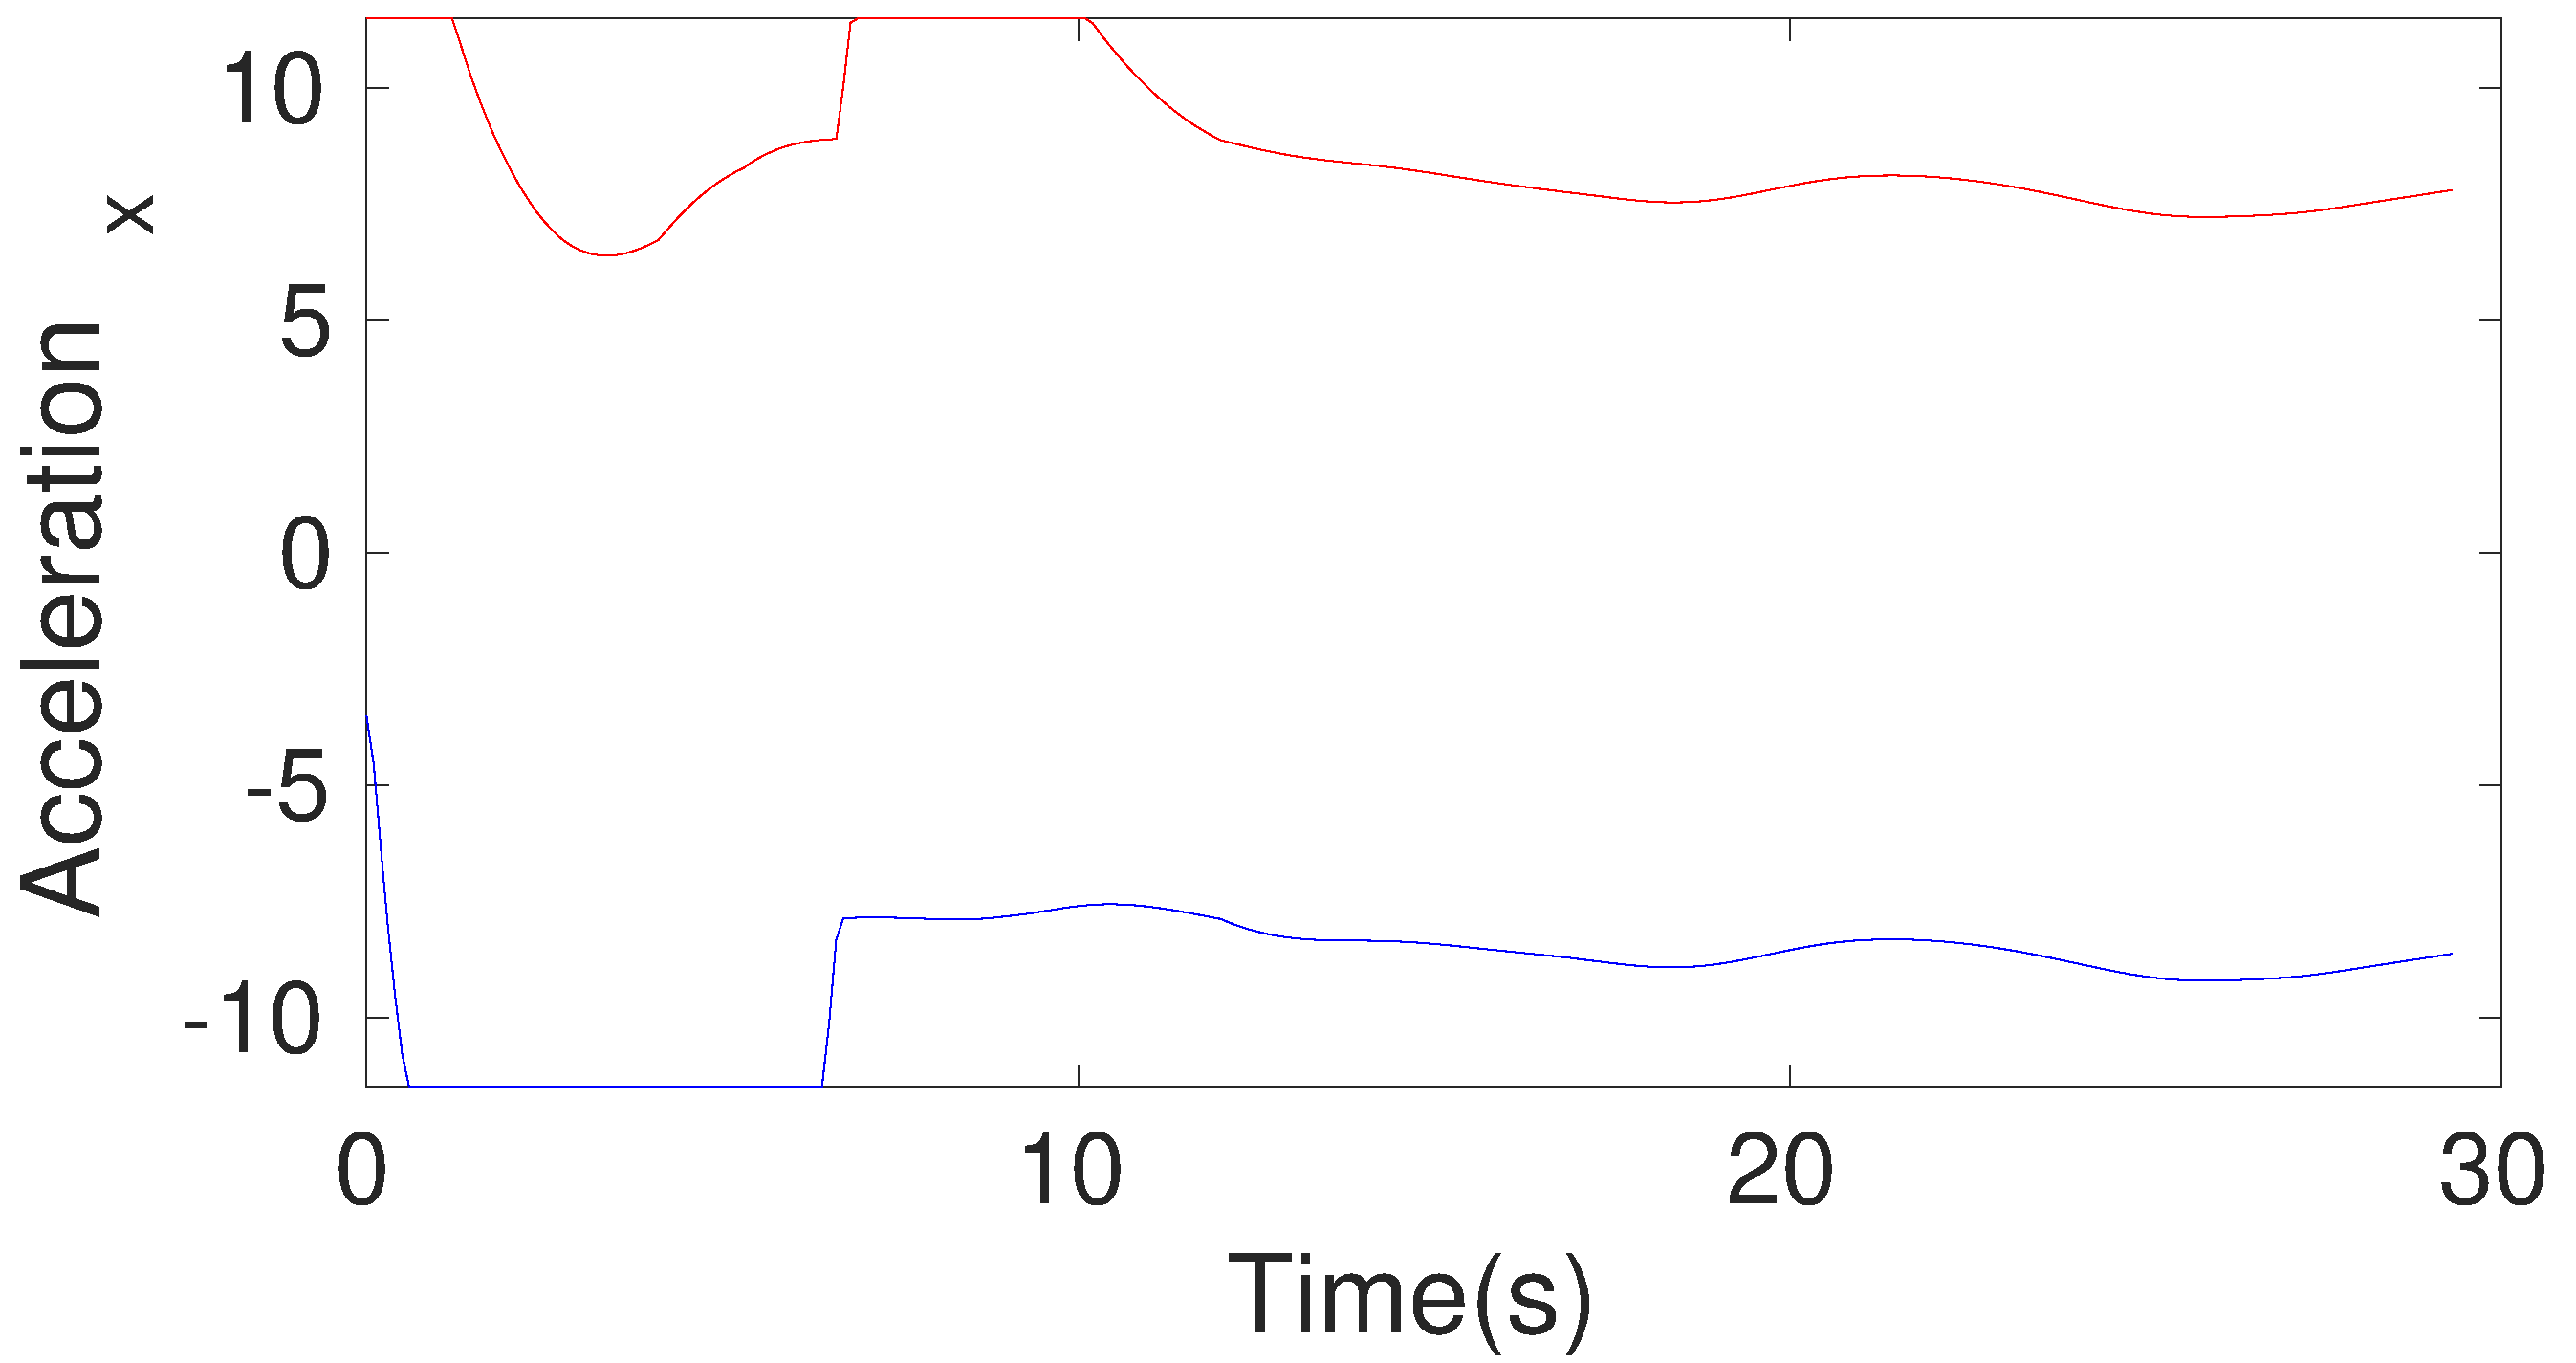
\includegraphics[width=\linewidth]{figures/Prad/s3pmpradAcceleration_x}
\end{subfigure}
\begin{subfigure}{.5\linewidth}
\centering
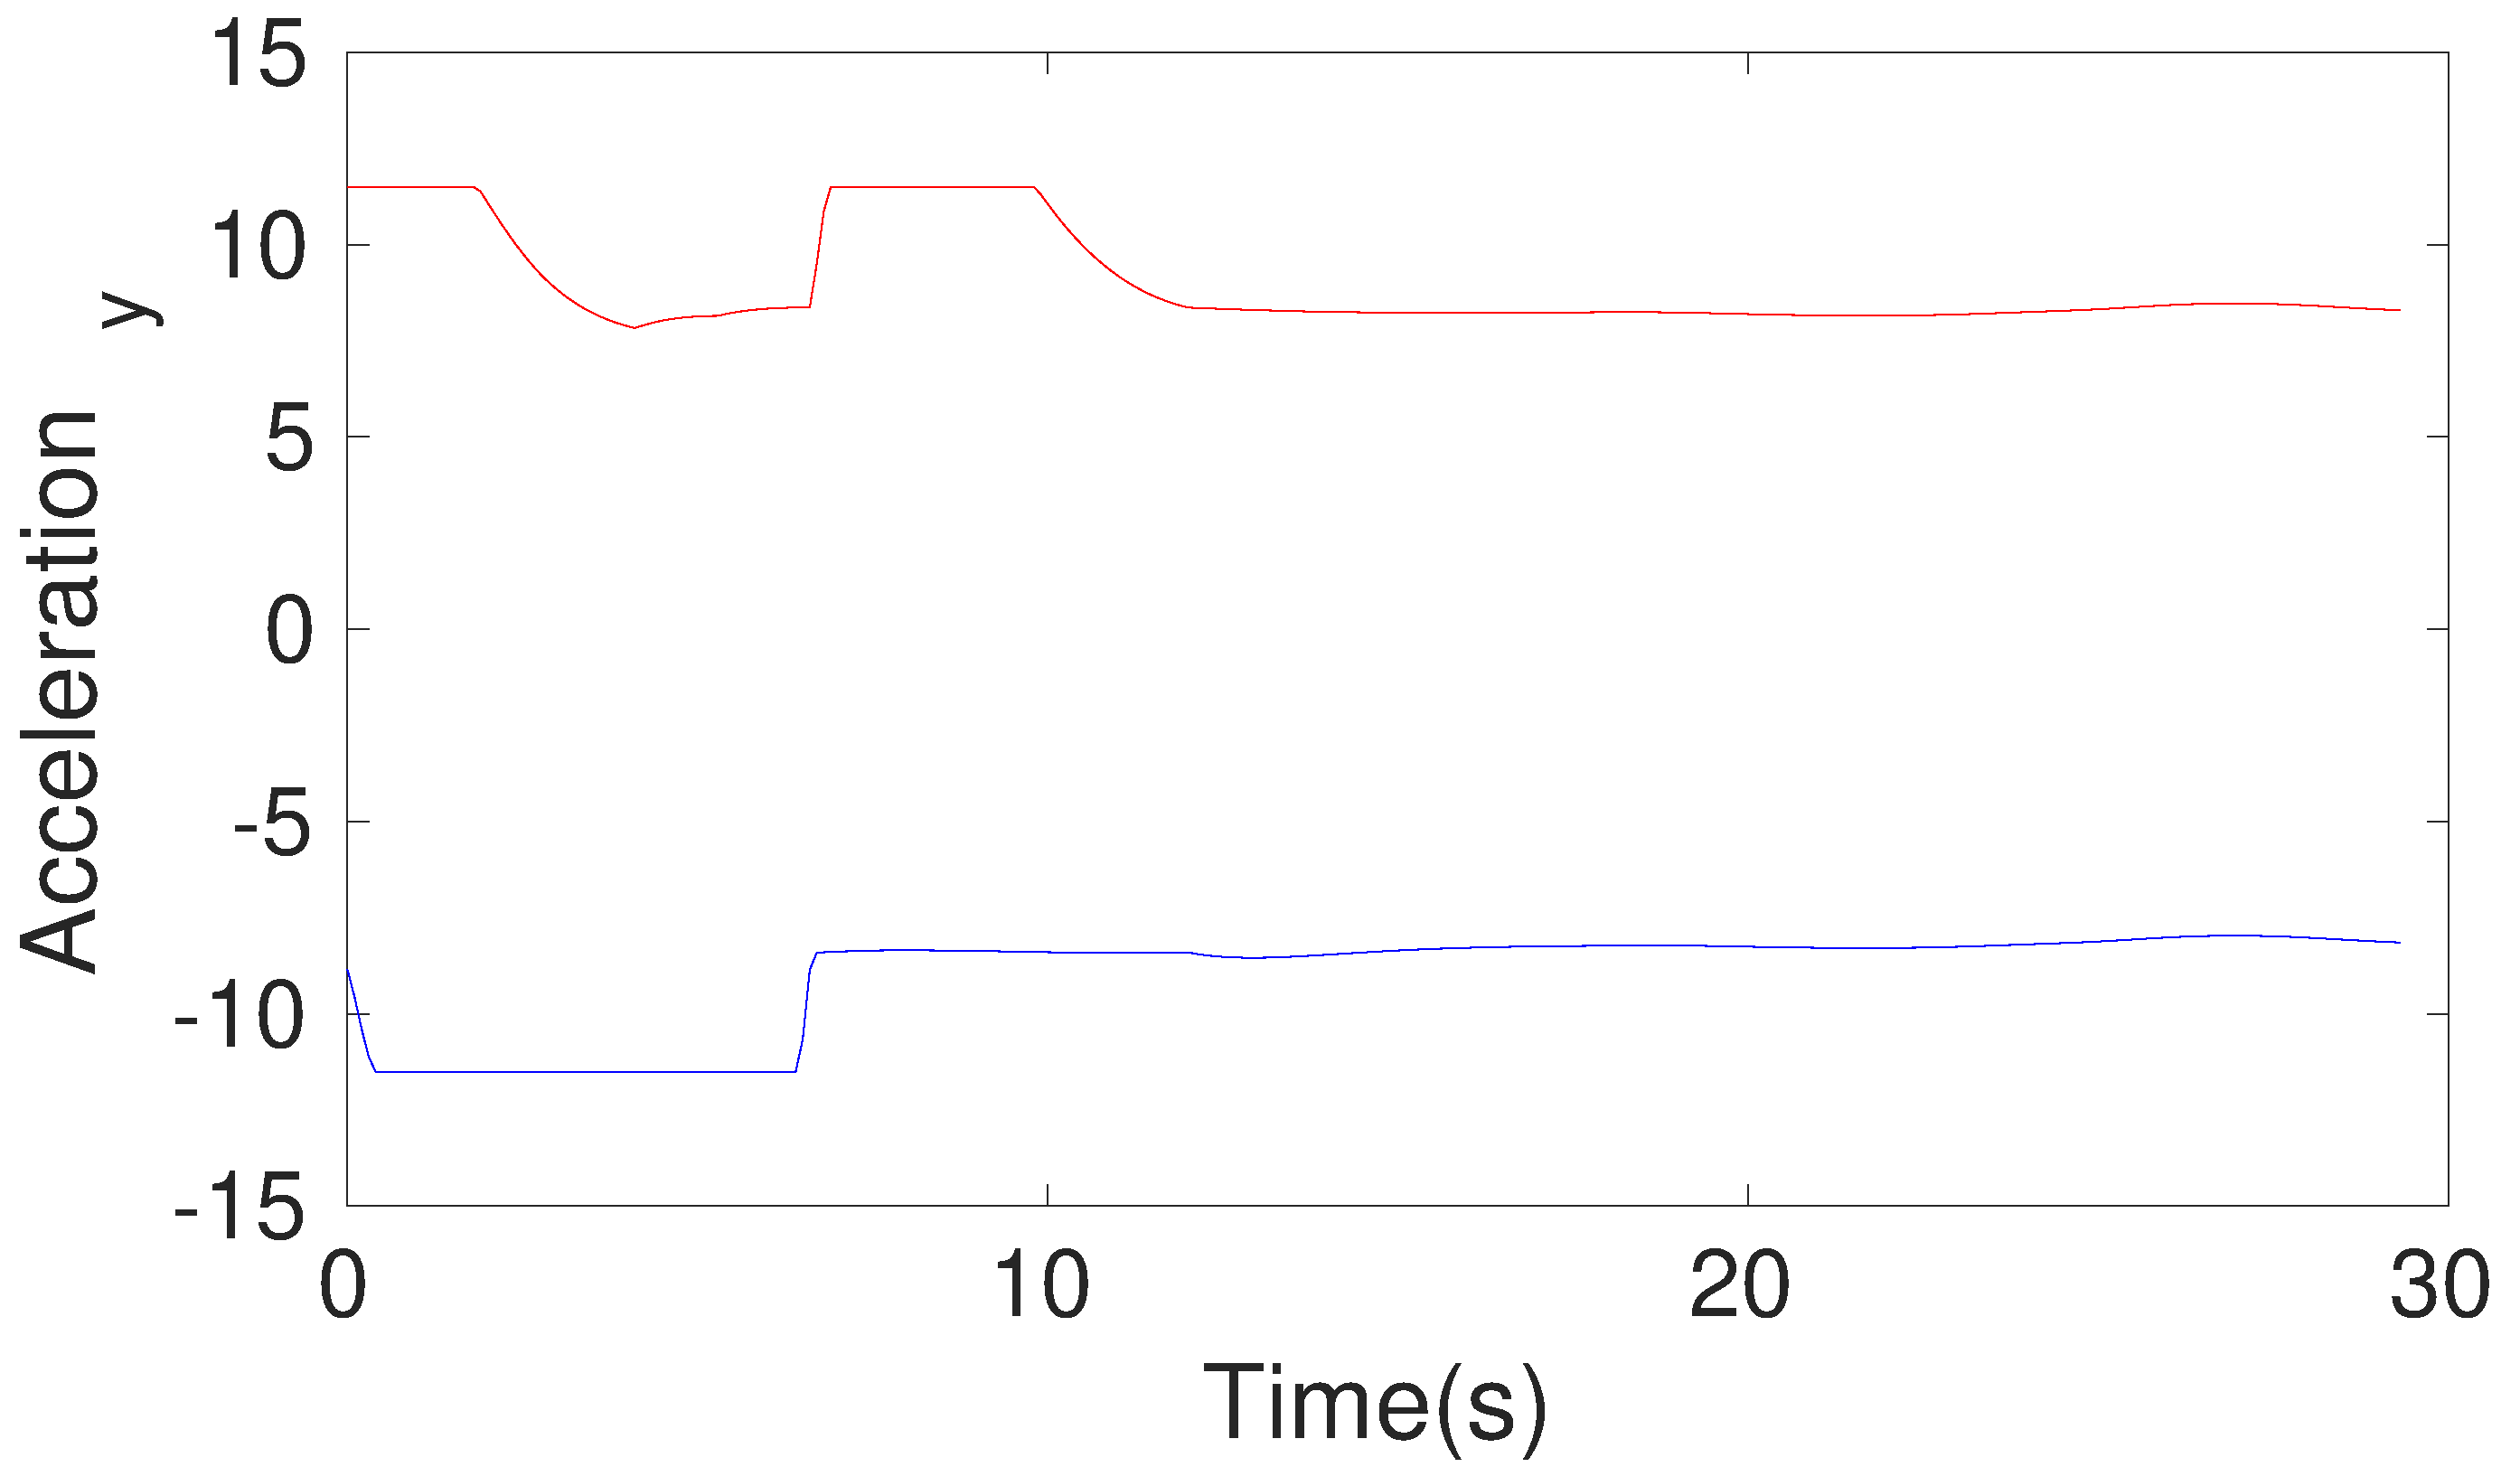
\includegraphics[width=\linewidth]{figures/Prad/s3pmpradAcceleration_y}
\end{subfigure}
\caption{Estimation using Point Mass Model}
\end{figure}


\clearpage
\subsubsection{Interval Observer using H-$\infty$}\label{eresult:hinf}
\FloatBarrier
\begin{figure}[!h]
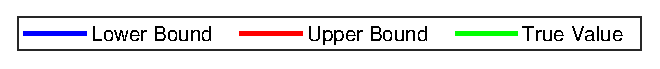
\includegraphics[scale=0.8]{figures/legend}\\\\
\begin{subfigure}{.5\linewidth}
\centering
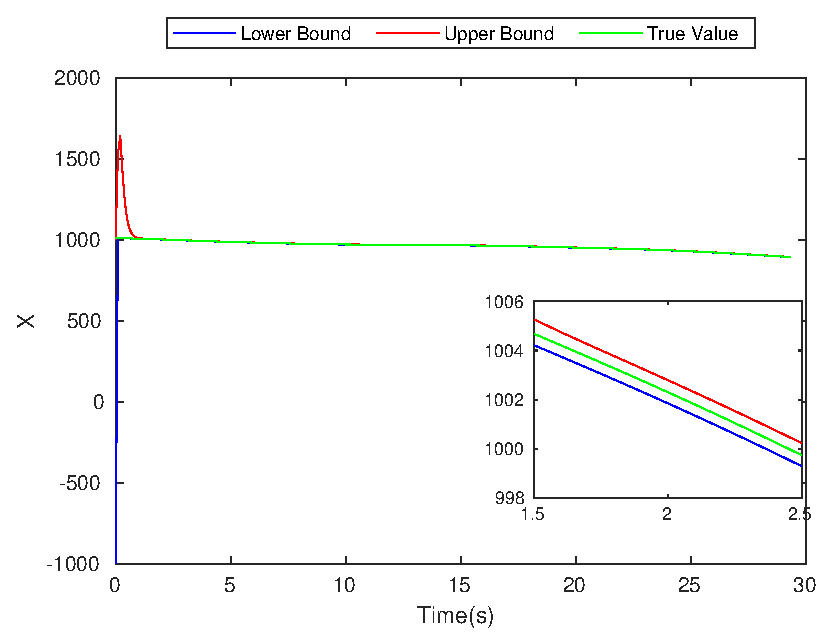
\includegraphics[width=\linewidth]{figures/HInf/s3cvHInfX}
\end{subfigure}
\begin{subfigure}{.5\linewidth}
\centering
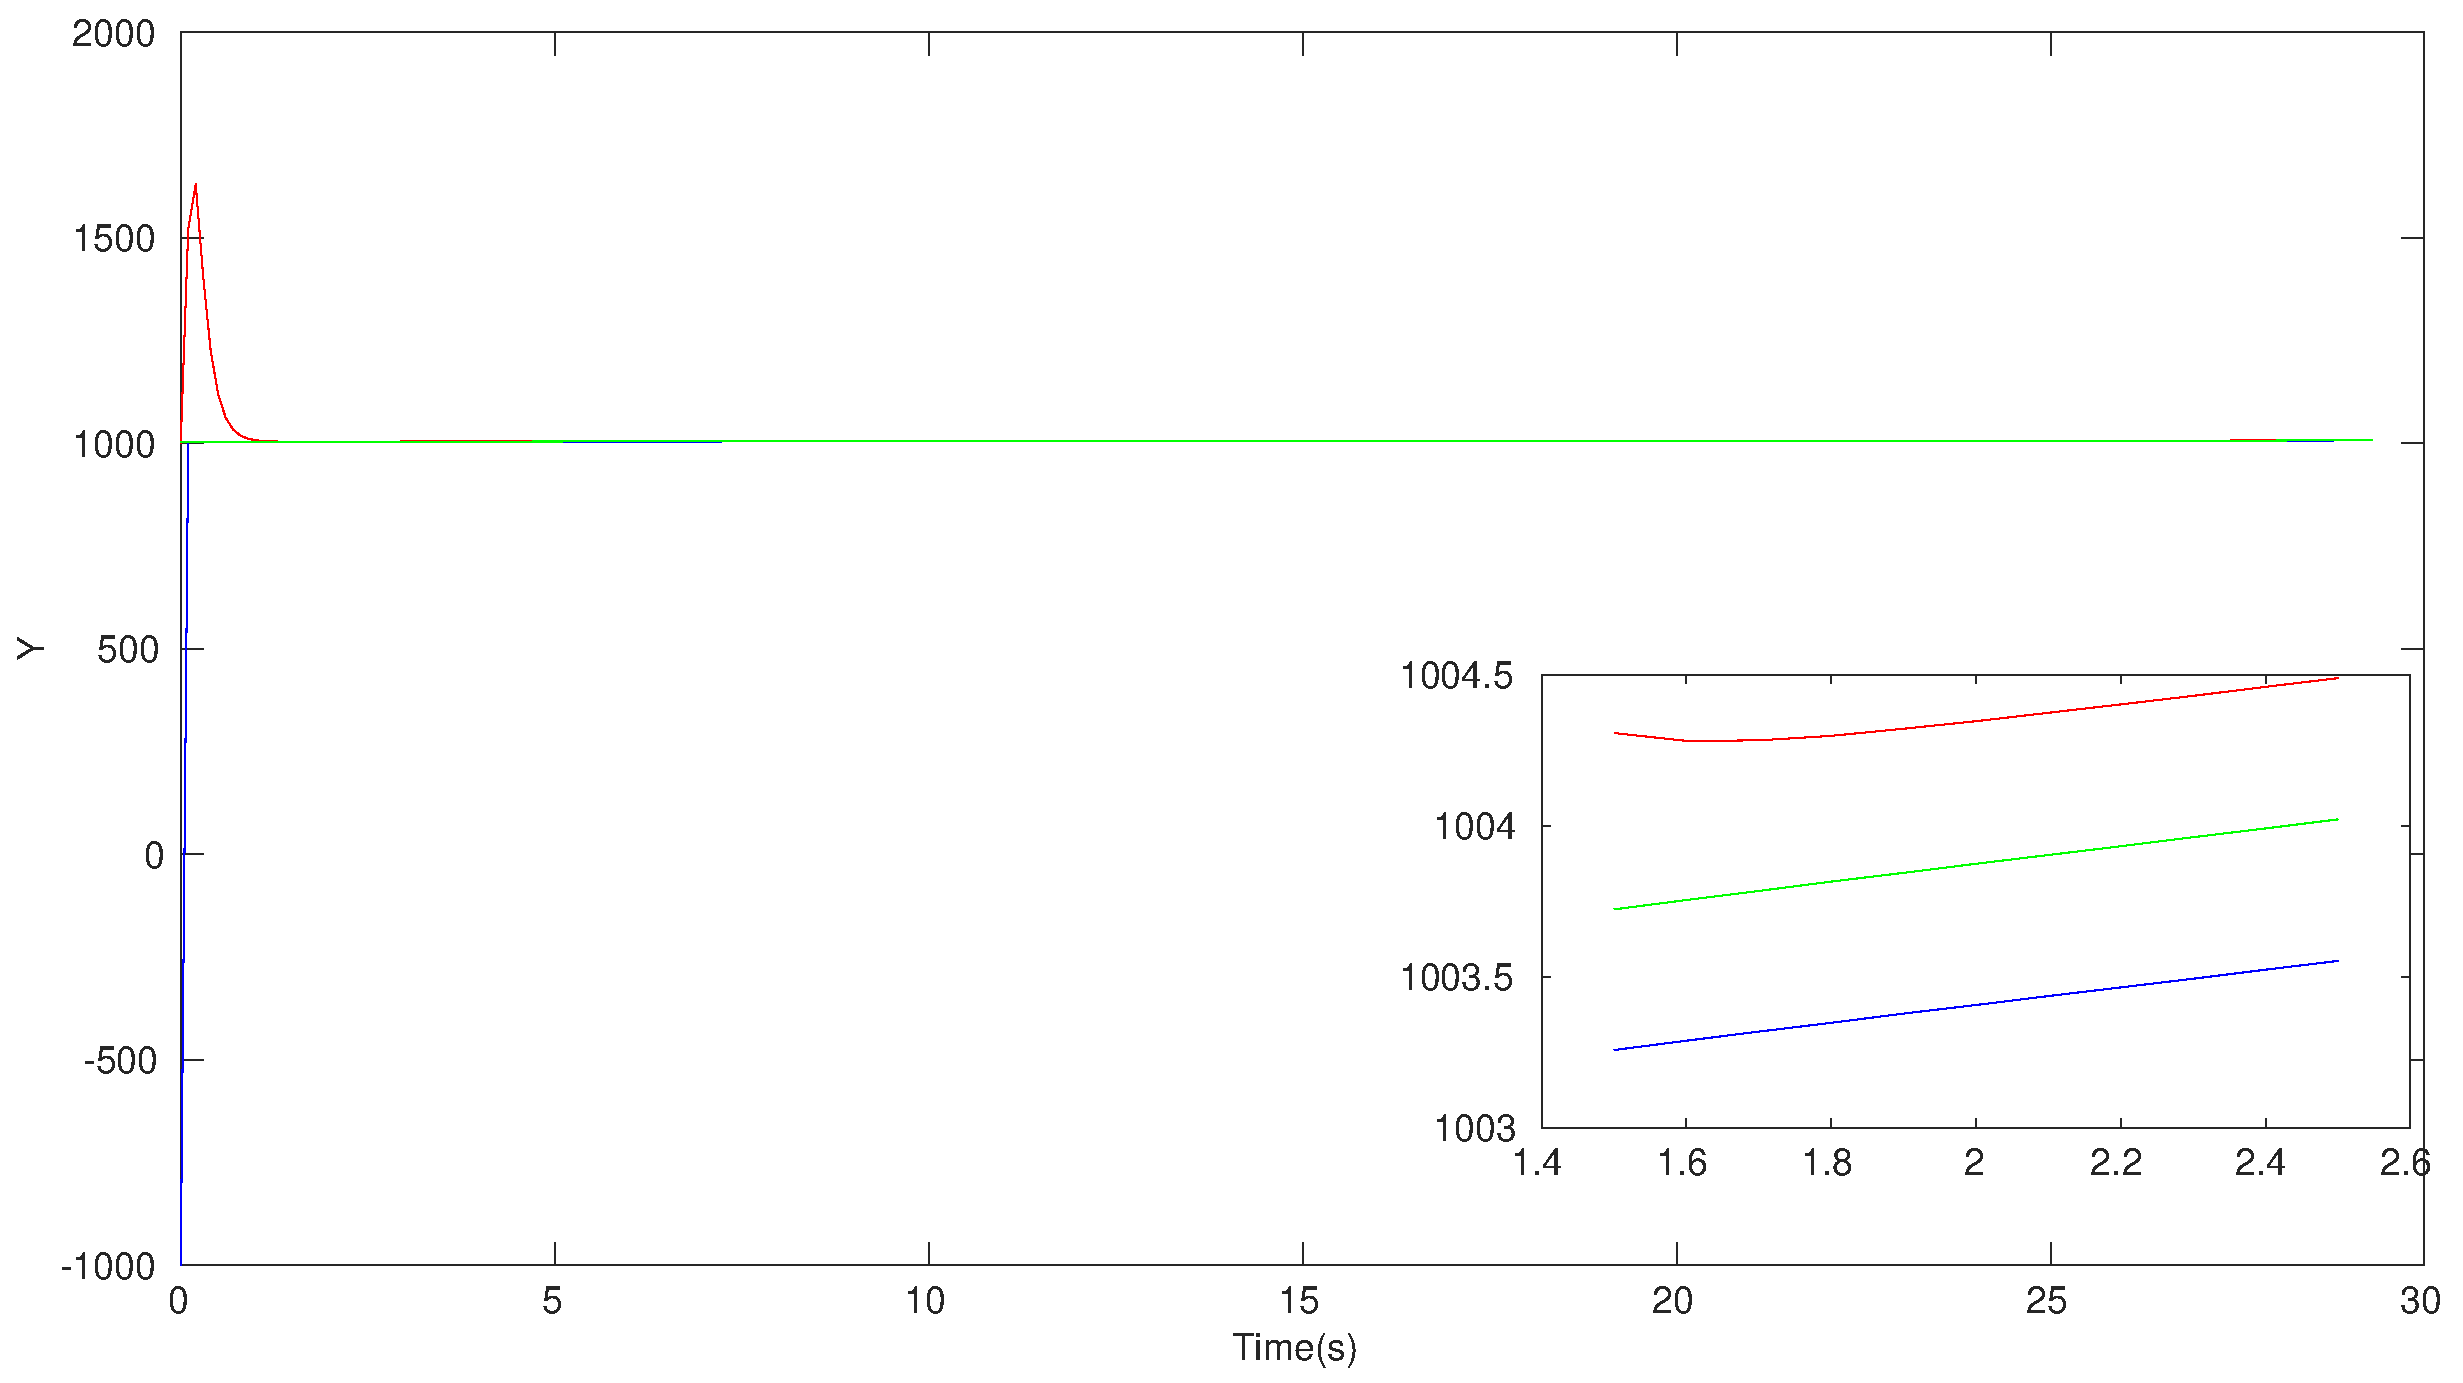
\includegraphics[width=\linewidth]{figures/HInf/s3cvHInfY}
\end{subfigure}
\begin{subfigure}{.5\linewidth}
\centering
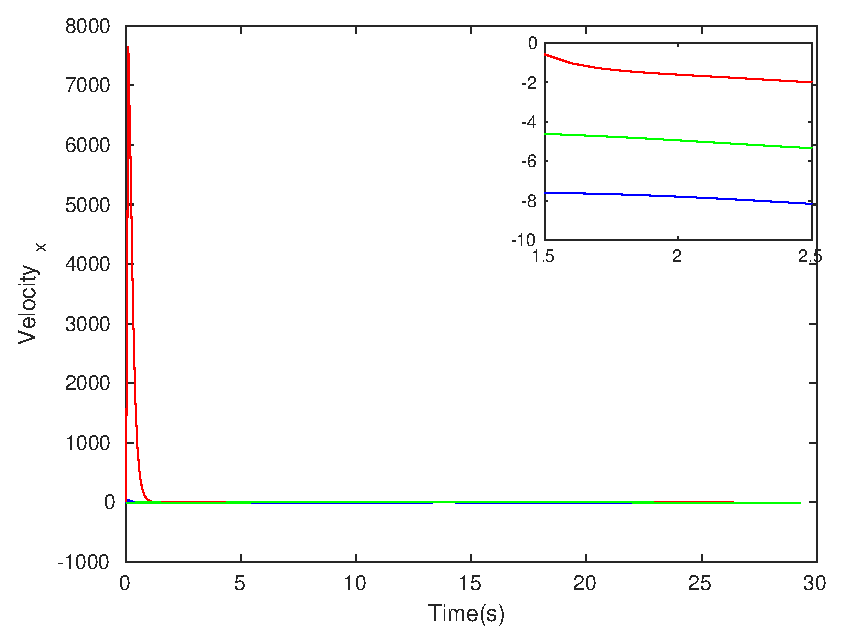
\includegraphics[width=\linewidth]{figures/HInf/s3cvHInfVelocity_x}
\end{subfigure}
\begin{subfigure}{.5\linewidth}
\centering
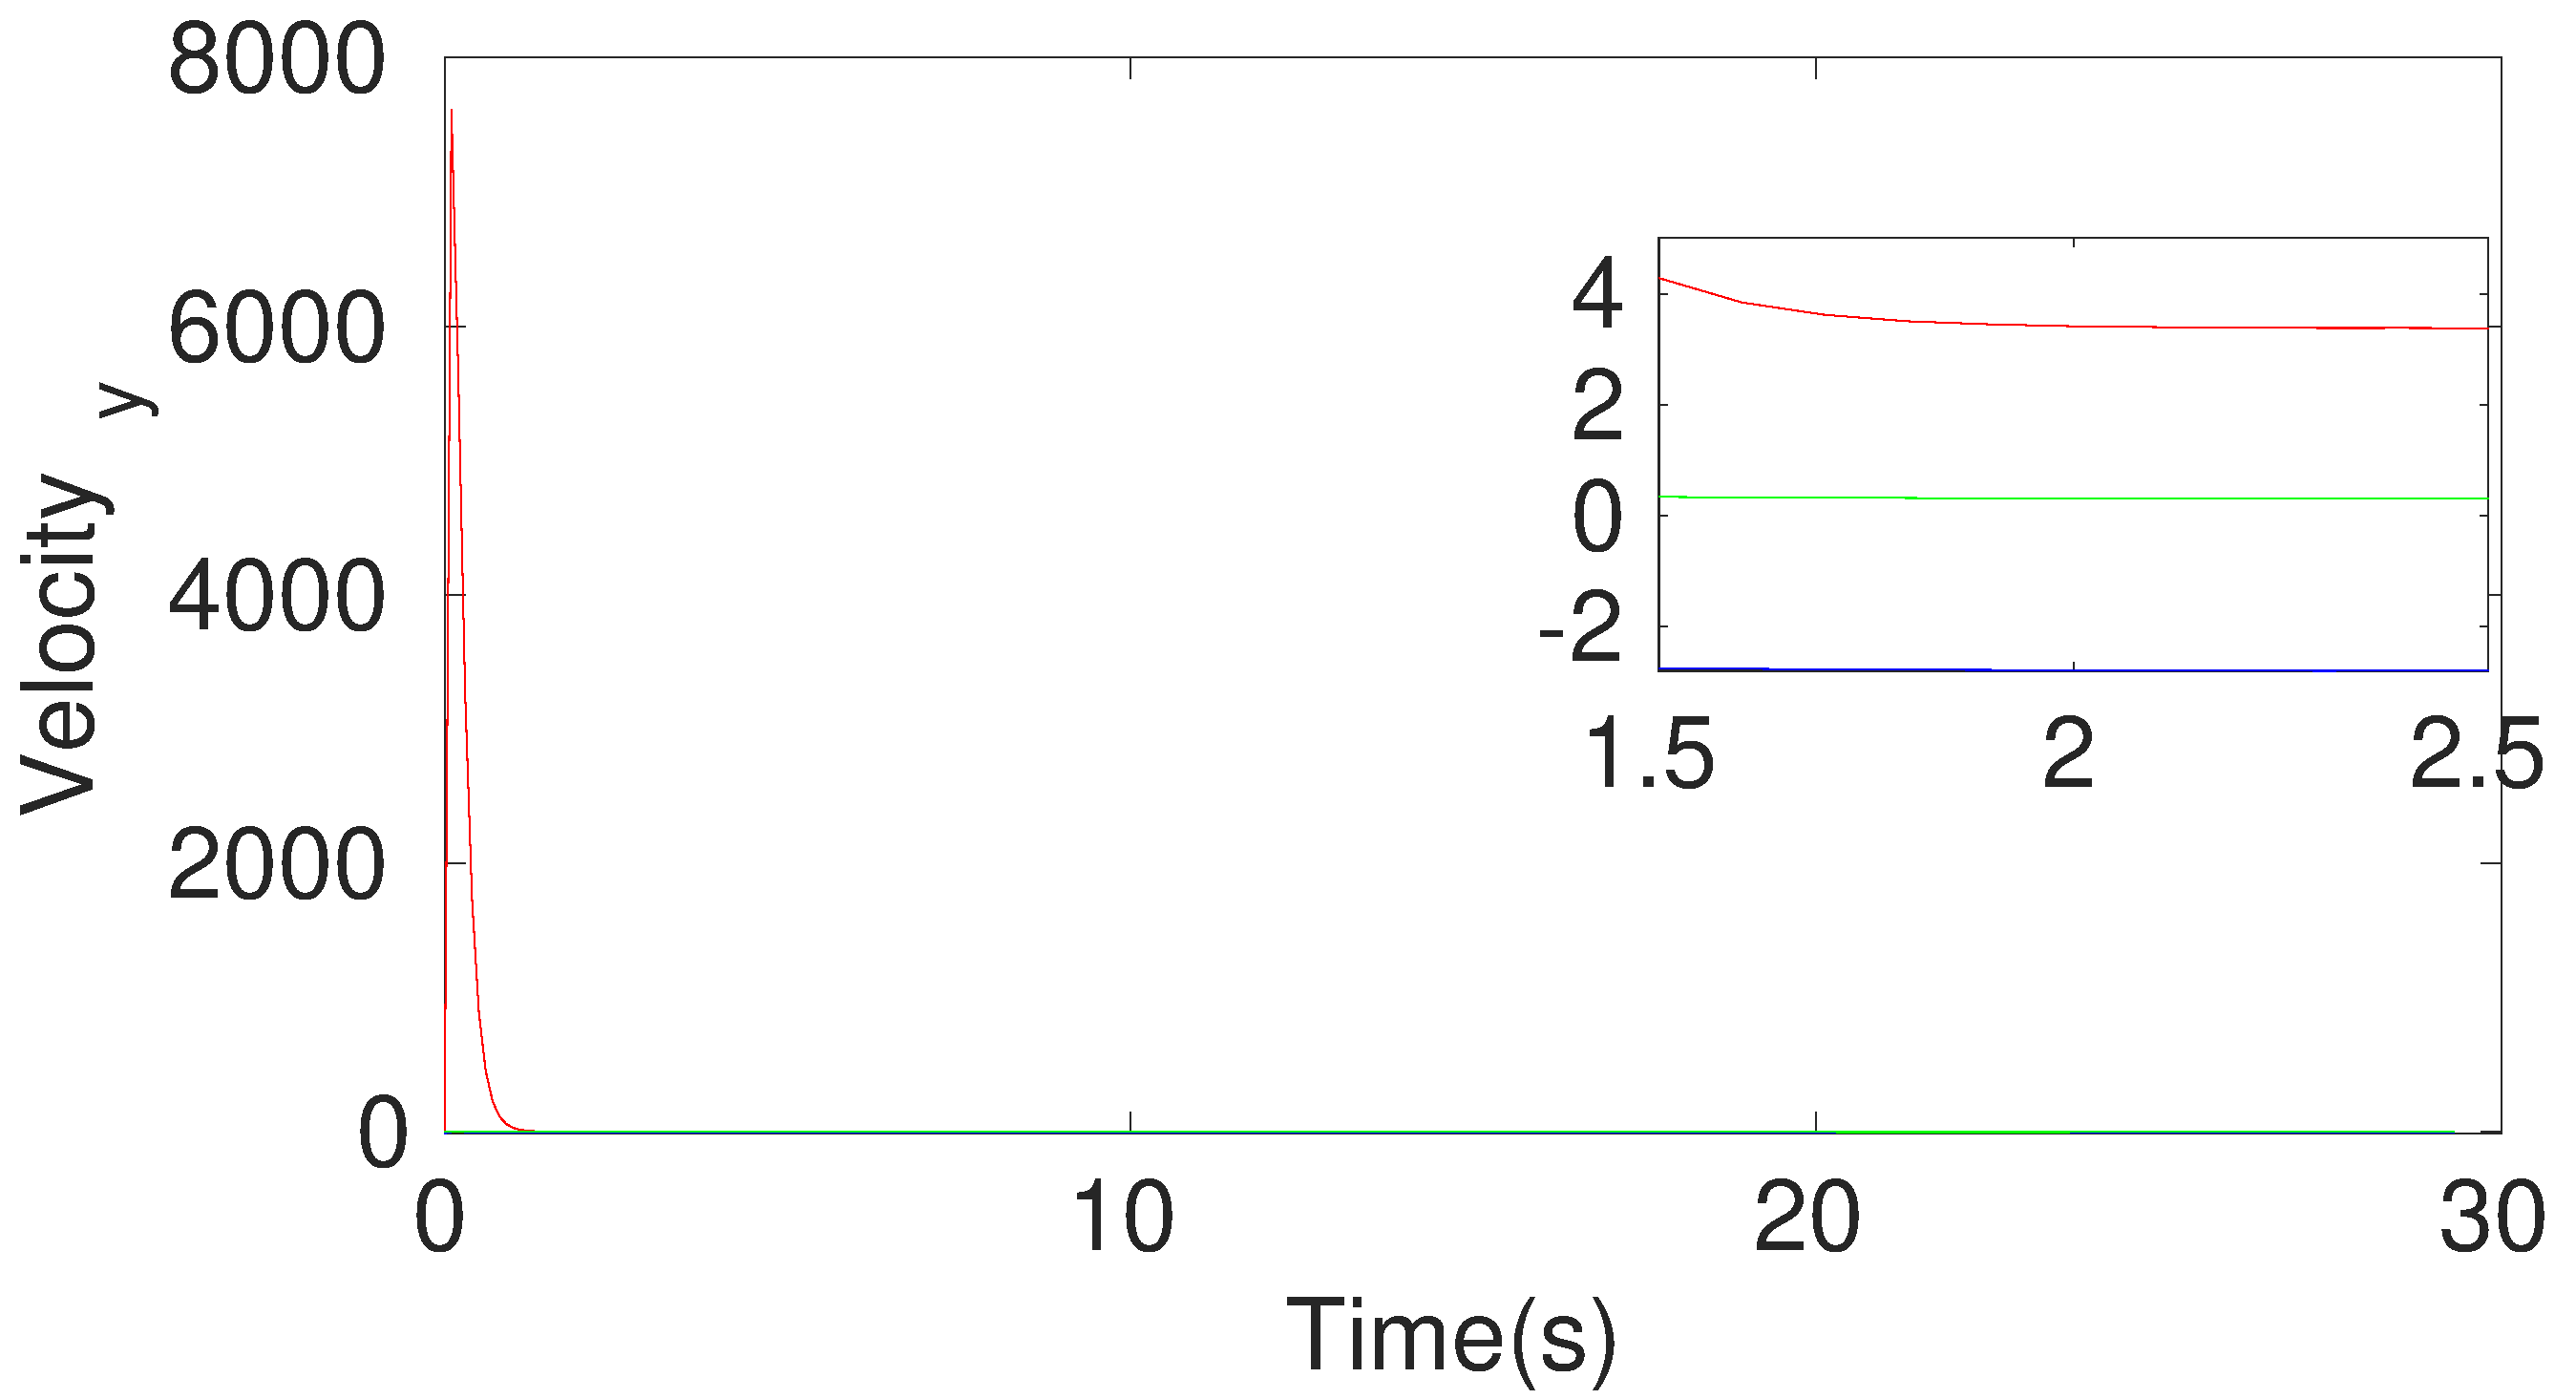
\includegraphics[width=\linewidth]{figures/HInf/s3cvHInfVelocity_y}
\end{subfigure}
\caption{Estimation using Constant Velocity}
\end{figure}

\begin{figure}[!h]
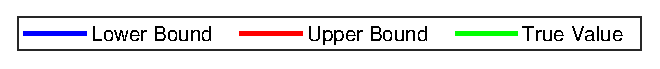
\includegraphics[scale=0.8]{figures/legend}\\\\
\begin{subfigure}{.5\linewidth}
\centering
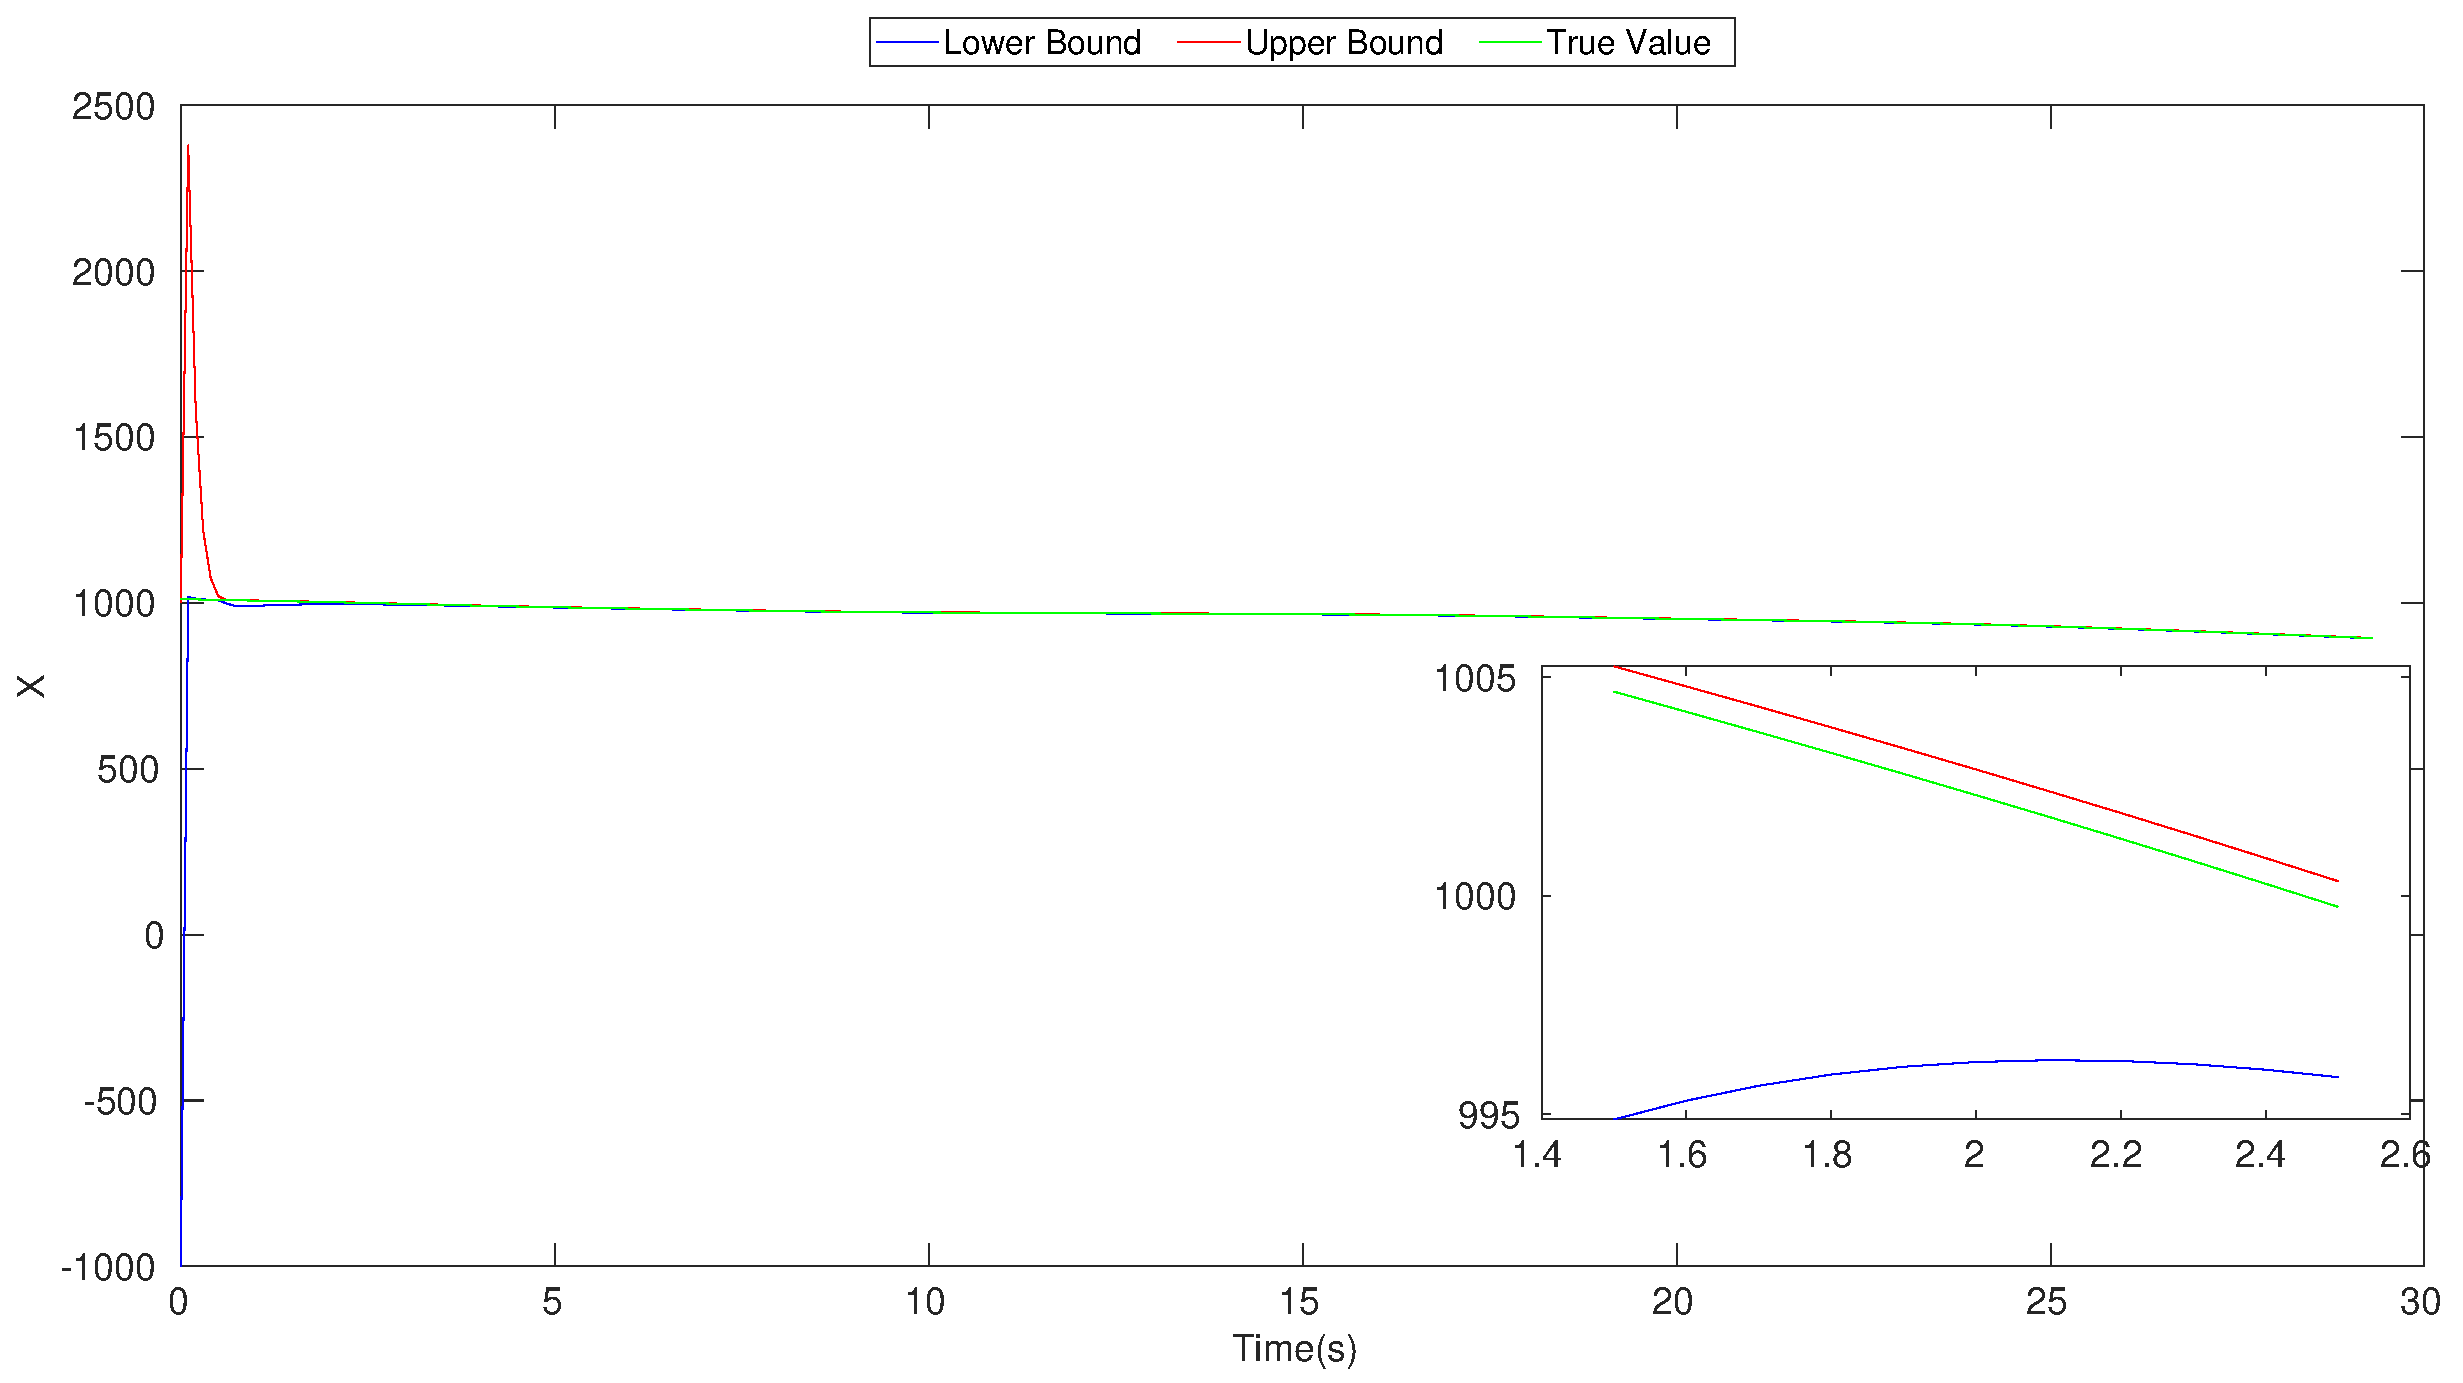
\includegraphics[width=\linewidth]{figures/HInf/s3caHInfX}
\end{subfigure}
\begin{subfigure}{.5\linewidth}
\centering
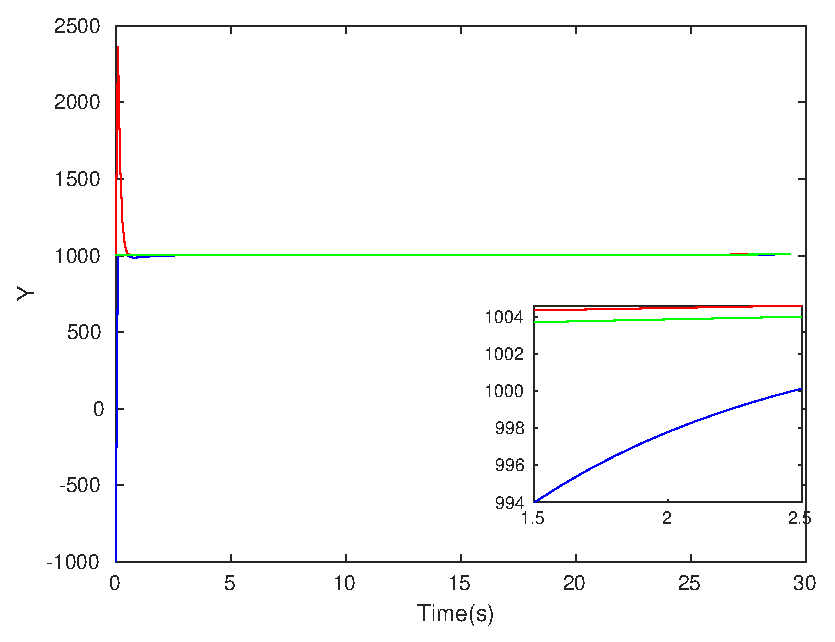
\includegraphics[width=\linewidth]{figures/HInf/s3caHInfY}
\end{subfigure}
\begin{subfigure}{.5\linewidth}
\centering
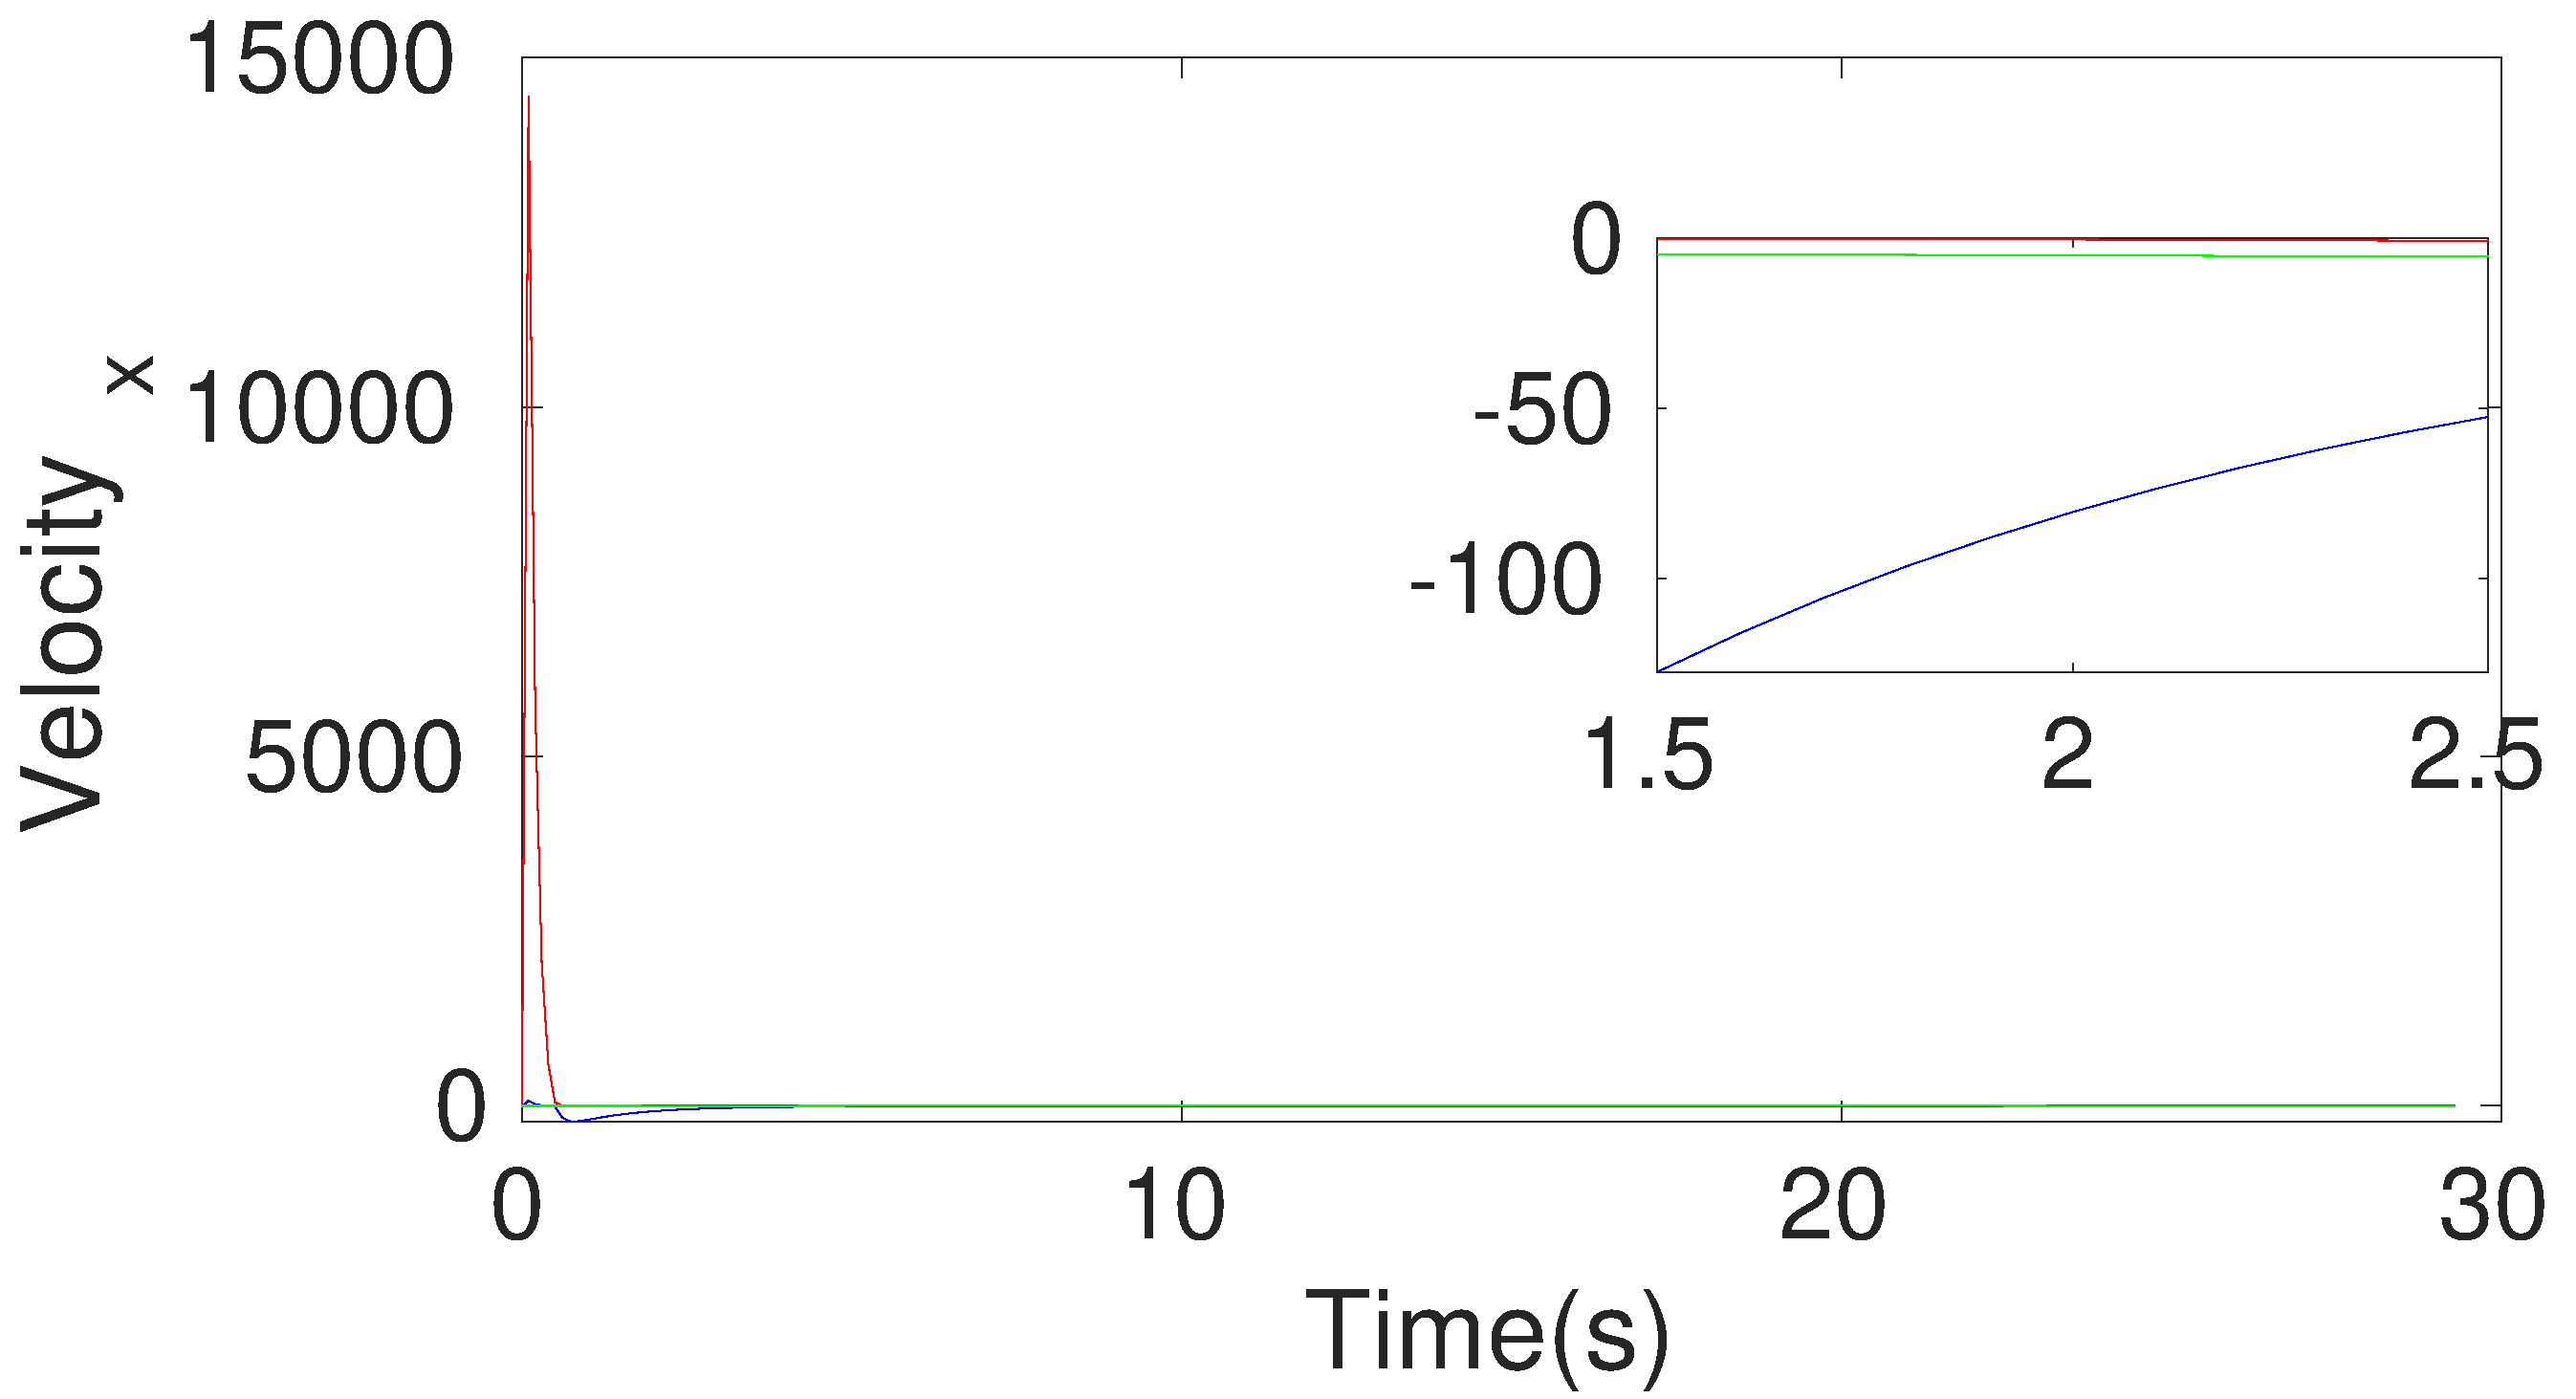
\includegraphics[width=\linewidth]{figures/HInf/s3caHInfVelocity_x}
\end{subfigure}
\begin{subfigure}{.5\linewidth}
\centering
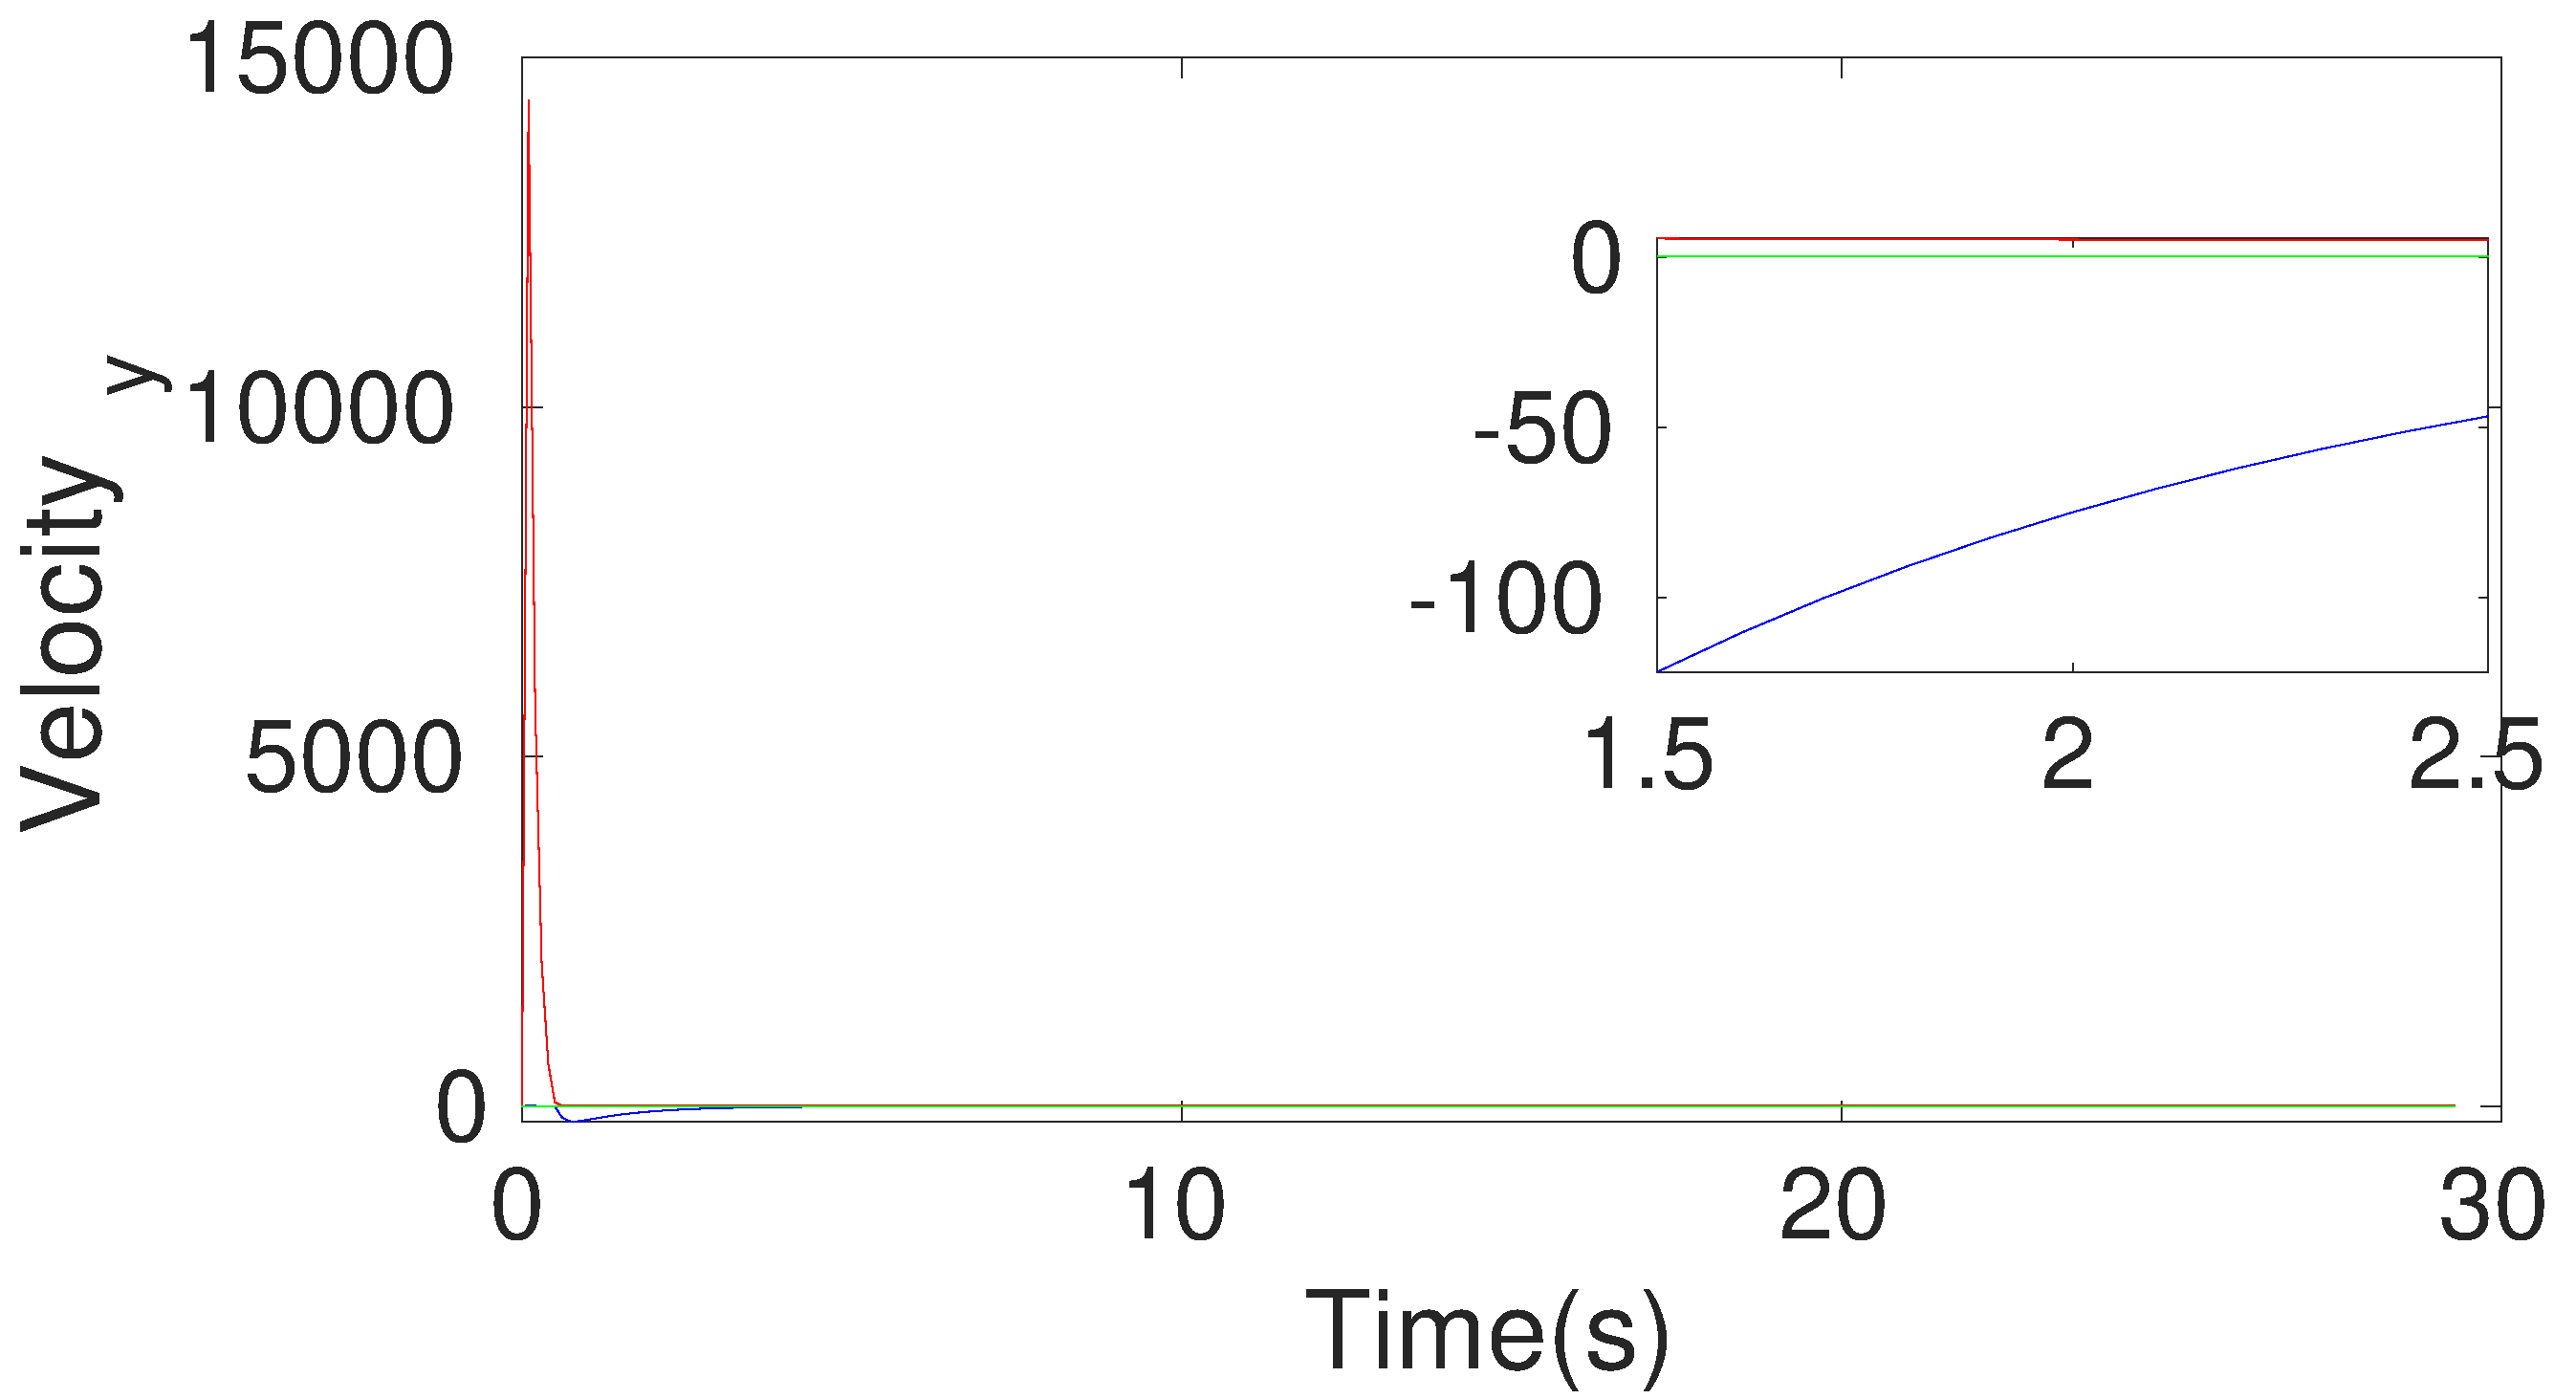
\includegraphics[width=\linewidth]{figures/HInf/s3caHInfVelocity_y}
\end{subfigure}
\begin{subfigure}{.5\linewidth}
\centering
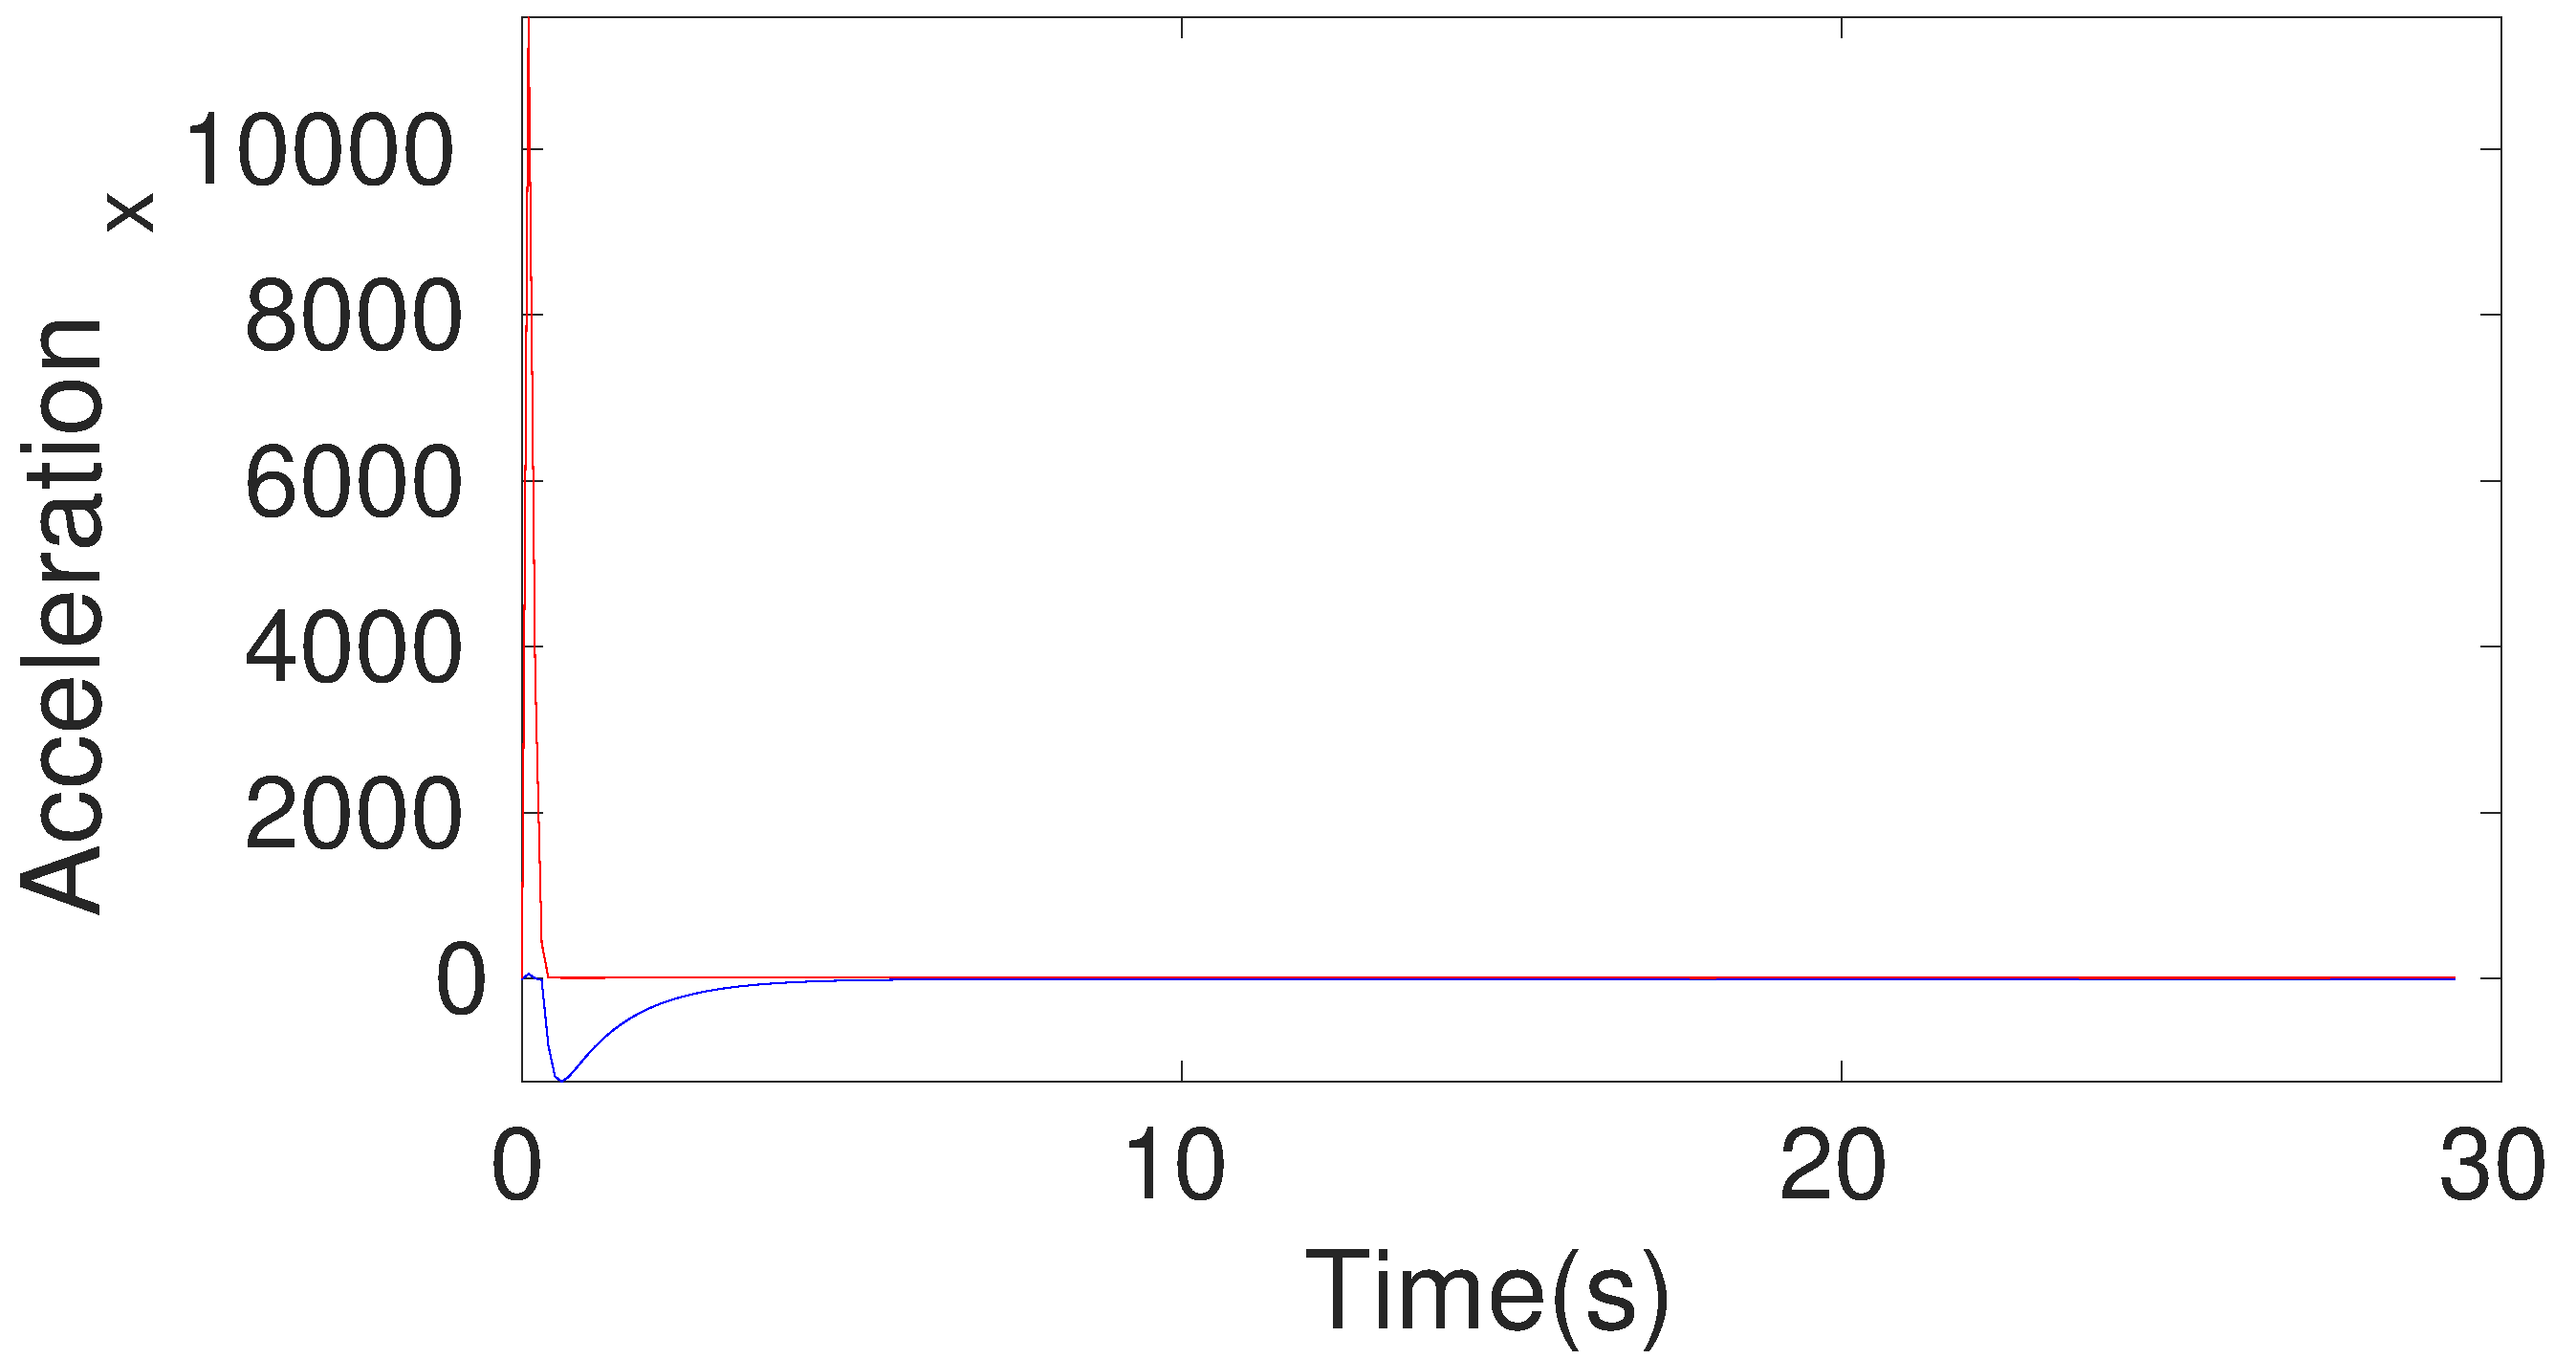
\includegraphics[width=\linewidth]{figures/HInf/s3caHInfAcceleration_x}
\end{subfigure}
\begin{subfigure}{.5\linewidth}
\centering
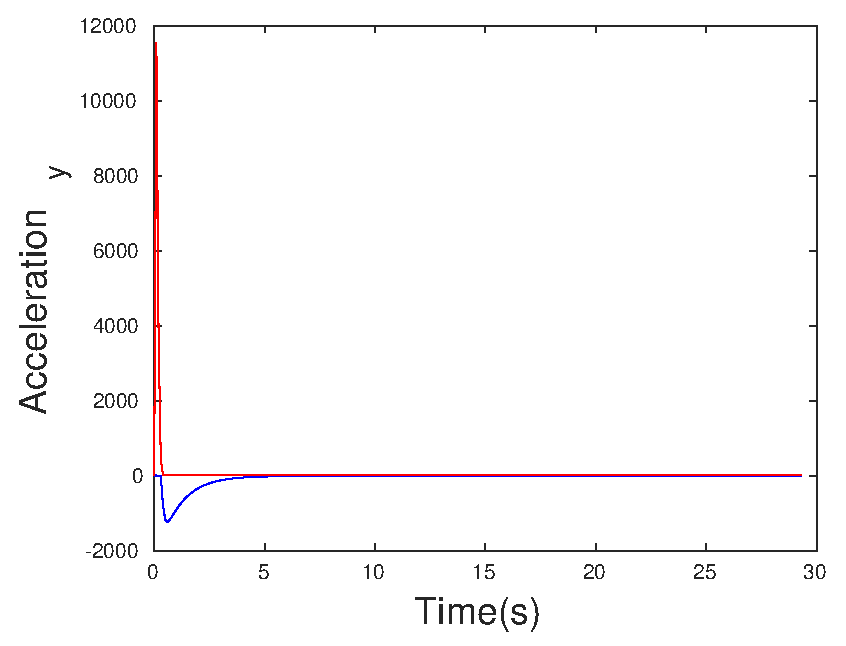
\includegraphics[width=\linewidth]{figures/HInf/s3caHInfAcceleration_y}
\end{subfigure}
\caption{Estimation using Constant Acceleration}
\end{figure}

\begin{figure}[!h]
\includegraphics[scale=0.8]{figures/legend}\\\\
\begin{subfigure}{.5\linewidth}
\centering
\includegraphics[width=\linewidth]{figures/HInf/s3pmHInfX}
\end{subfigure}
\begin{subfigure}{.5\linewidth}
\centering
\includegraphics[width=\linewidth]{figures/HInf/s3pmHInfY}
\end{subfigure}
\begin{subfigure}{.5\linewidth}
\centering
\includegraphics[width=\linewidth]{figures/HInf/s3pmHInfVelocity_x}
\end{subfigure}
\begin{subfigure}{.5\linewidth}
\centering
\includegraphics[width=\linewidth]{figures/HInf/s3pmHInfVelocity_y}
\end{subfigure}
\begin{subfigure}{.5\linewidth}
\centering
\includegraphics[width=\linewidth]{figures/HInf/s3pmHInfAcceleration_x}
\end{subfigure}
\begin{subfigure}{.5\linewidth}
\centering
\includegraphics[width=\linewidth]{figures/HInf/s3pmHInfAcceleration_y}
\end{subfigure}
\caption{Estimation using Point Mass Model}
\end{figure}

\subsection{Rate of Change of Bounds}\label{eresult:rate}
\FloatBarrier
\begin{figure}[!h]
\includegraphics[scale=0.8]{figures/ratelegend}\\\\
\begin{subfigure}{.5\linewidth}
\centering
\includegraphics[width=\linewidth]{figures/BoundChange/CV/cv_bound_changeX}
\end{subfigure}
\begin{subfigure}{.5\linewidth}
\centering
\includegraphics[width=\linewidth]{figures/BoundChange/CV/cv_bound_changeY}
\end{subfigure}
\begin{subfigure}{.5\linewidth}
\centering
\includegraphics[width=\linewidth]{figures/BoundChange/CV/cv_bound_changeVelocity_x}
\end{subfigure}
\begin{subfigure}{.5\linewidth}
\centering
\includegraphics[width=\linewidth]{figures/BoundChange/CV/cv_bound_changeVelocity_y}
\end{subfigure}
\caption{Rate of change of bounds using Constant Velocity Model}
\end{figure}

\begin{figure}[!h]
\includegraphics[scale=0.8]{figures/ratelegend}\\\\
\begin{subfigure}{.5\linewidth}
\centering
\includegraphics[width=\linewidth]{figures/BoundChange/CA/ca_bound_changeX}
\end{subfigure}
\begin{subfigure}{.5\linewidth}
\centering
\includegraphics[width=\linewidth]{figures/BoundChange/CA/ca_bound_changeY}
\end{subfigure}
\begin{subfigure}{.5\linewidth}
\centering
\includegraphics[width=\linewidth]{figures/BoundChange/CA/ca_bound_changeVelocity_x}
\end{subfigure}
\begin{subfigure}{.5\linewidth}
\centering
\includegraphics[width=\linewidth]{figures/BoundChange/CA/ca_bound_changeVelocity_y}
\end{subfigure}
\begin{subfigure}{.5\linewidth}
\centering
\includegraphics[width=\linewidth]{figures/BoundChange/CA/ca_bound_changeAcceleration_x}
\end{subfigure}
\begin{subfigure}{.5\linewidth}
\centering
\includegraphics[width=\linewidth]{figures/BoundChange/CA/ca_bound_changeAcceleration_y}
\end{subfigure}
\caption{Rate of change of bounds using Constant Acceleration Model}
\end{figure}

\begin{figure}[!h]
\includegraphics[scale=0.8]{figures/ratelegend}\\\\
\begin{subfigure}{.5\linewidth}
\centering
\includegraphics[width=\linewidth]{figures/BoundChange/PM/pm_bound_changeX}
\end{subfigure}
\begin{subfigure}{.5\linewidth}
\centering
\includegraphics[width=\linewidth]{figures/BoundChange/PM/pm_bound_changeY}
\end{subfigure}
\begin{subfigure}{.5\linewidth}
\centering
\includegraphics[width=\linewidth]{figures/BoundChange/PM/pm_bound_changeVelocity_x}
\end{subfigure}
\begin{subfigure}{.5\linewidth}
\centering
\includegraphics[width=\linewidth]{figures/BoundChange/PM/pm_bound_changeVelocity_y}
\end{subfigure}
\begin{subfigure}{.5\linewidth}
\centering
\includegraphics[width=\linewidth]{figures/BoundChange/PM/pm_bound_changeAcceleration_x}
\end{subfigure}
\begin{subfigure}{.5\linewidth}
\centering
\includegraphics[width=\linewidth]{figures/BoundChange/PM/pm_bound_changeAcceleration_y}
\end{subfigure}
\caption{Rate of change of bounds using Point-Mass Model}
\end{figure}
\pagebreak
\section{Template Code}
\subsection{Template for Model}
% This file was automatically created from the m-file 
% "m2tex.m" written by USL. 
% The fontencoding in this file is UTF-8. 
%  
% You will need to include the following two packages in 
% your LaTeX-Main-File. 
%  
% \usepackage{color} 
% \usepackage{fancyvrb} 
%  
% It is advised to use the following option for Inputenc 
% \usepackage[utf8]{inputenc} 
%  
  
% definition of matlab colors: 
\definecolor{mblue}{rgb}{0,0,1} 
\definecolor{mgreen}{rgb}{0.13333,0.5451,0.13333} 
\definecolor{mred}{rgb}{0.62745,0.12549,0.94118} 
\definecolor{mgrey}{rgb}{0.5,0.5,0.5} 
\definecolor{mdarkgrey}{rgb}{0.25,0.25,0.25} 
  
\DefineShortVerb[fontfamily=courier,fontseries=m]{\$} 
\DefineShortVerb[fontfamily=courier,fontseries=b]{\#} 
  
\noindent                            
 $$\color{mblue}$classdef$\color{black}$ Model$\\
 $    $\color{mgreen}$%MODEL Model Template$\color{black}$$\\
 $    $\color{mgreen}$%   dim_x: estimate dimension$\color{black}$$\\
 $    $\color{mgreen}$%   dim_y: measurement dimension$\color{black}$$\\
 $    $\\
 $    properties$\\
 $        A$\\
 $        C$\\
 $        W$\\
 $        V$\\
 $        initial$\\
 $        dim_x;$\\
 $        dim_;$\\
 $        delT = 0.1;$\\
 $    $\color{mblue}$end$\color{black}$$\\
 $    $\\
 $    methods$\\
 $        $\color{mblue}$function$\color{black}$ obj = Model(delT)$\\
 $            $\color{mgreen}$%MODEL Construct an instance of this class$\color{black}$$\\
 $            $\color{mgreen}$%   Initializes the model variables$\color{black}$$\\
 $            obj.delT = delT; $\color{mgreen}$% add the time step$\color{black}$$\\
 $            $\\
 $            $\color{mgreen}$% Assign parameters here$\color{black}$$\\
 $        $\color{mblue}$end$\color{black}$$\\
 $    $\color{mblue}$end$\color{black}$$\\
 $$\color{mblue}$end$\color{black}$$\\
 $$\\
 $$\\ 
  
\UndefineShortVerb{\$} 
\UndefineShortVerb{\#}
\pagebreak
\subsection{Template for Estimator}
% This file was automatically created from the m-file 
% "m2tex.m" written by USL. 
% The fontencoding in this file is UTF-8. 
%  
% You will need to include the following two packages in 
% your LaTeX-Main-File. 
%  
% \usepackage{color} 
% \usepackage{fancyvrb} 
%  
% It is advised to use the following option for Inputenc 
% \usepackage[utf8]{inputenc} 
%  
  
% definition of matlab colors: 
\definecolor{mblue}{rgb}{0,0,1} 
\definecolor{mgreen}{rgb}{0.13333,0.5451,0.13333} 
\definecolor{mred}{rgb}{0.62745,0.12549,0.94118} 
\definecolor{mgrey}{rgb}{0.5,0.5,0.5} 
\definecolor{mdarkgrey}{rgb}{0.25,0.25,0.25} 
  
\DefineShortVerb[fontfamily=courier,fontseries=m]{\$} 
\DefineShortVerb[fontfamily=courier,fontseries=b]{\#} 
  
\noindent                                     
 $$\color{mblue}$classdef$\color{black}$ Estimator < handle$\\
 $    $\color{mgreen}$%ESTIMATOR Estimator template$\color{black}$$\\
 $    $\color{mgreen}$%   model: model to represent vehicle dynamics$\color{black}$$\\
 $    $\\
 $    properties$\\
 $        model$\\
 $        E$\\
 $        F$\\
 $        x_estimated$\\
 $        index$\\
 $    $\color{mblue}$end$\color{black}$$\\
 $    $\\
 $    methods$\\
 $        $\color{mblue}$function$\color{black}$ obj = Estimator(model)$\\
 $            $\color{mgreen}$%ESTIMATOR Constructor$\color{black}$$\\
 $            $\color{mgreen}$% Initialize variables$\color{black}$$\\
 $            obj.model = model;$\\
 $            obj.index = 1; $\color{mgreen}$% keep track of measurements$\color{black}$$\\
 $            $\\
 $            $\color{mgreen}$% initialize variables here$\color{black}$$\\
 $            $\\
 $            $\color{mgreen}$% implement initial computation $\color{black}$$\\
 $        $\color{mblue}$end$\color{black}$$\\
 $        $\\
 $        $\color{mblue}$function$\color{black}$ [x_lower, x_upper] = estimate(obj, y)$\\
 $            $\color{mgreen}$%ESTIMATE estimate from the measurement$\color{black}$$\\
 $            $\\
 $            $\color{mgreen}$% implement estimator algorithm on measurement, y$\color{black}$$\\
 $            $\\
 $            $\color{mgreen}$% return bounds$\color{black}$$\\
 $            x_lower = 0;$\\
 $            x_upper = 0;$\\
 $        $\color{mblue}$end$\color{black}$$\\
 $        $\\
 $    $\color{mblue}$end$\color{black}$$\\
 $$\color{mblue}$end$\color{black}$$\\
 $$\\ 
  
\UndefineShortVerb{\$} 
\UndefineShortVerb{\#}
%\end{appendices}
